% This LaTeX document needs to be compiled with XeLaTeX.
\documentclass[10pt]{article}
\usepackage[utf8]{inputenc}
\usepackage{ucharclasses}
\usepackage{amsmath}
\usepackage{amsfonts}
\usepackage{amssymb}
\usepackage[version=4]{mhchem}
\usepackage{stmaryrd}
\usepackage{graphicx}
\usepackage[export]{adjustbox}
\graphicspath{ {./images/} }
\usepackage{caption}
\usepackage[fallback]{xeCJK}
\usepackage{polyglossia}
\usepackage{fontspec}
\IfFontExistsTF{Noto Serif CJK TC}
{\setCJKmainfont{Noto Serif CJK TC}}
{\IfFontExistsTF{STSong}
  {\setCJKmainfont{STSong}}
  {\IfFontExistsTF{Droid Sans Fallback}
    {\setCJKmainfont{Droid Sans Fallback}}
    {\setCJKmainfont{SimSun}}
}}

\setmainlanguage{vietnamese}
\setotherlanguages{english}
\newfontfamily\vietnamesefont{CMU Serif}
\IfFontExistsTF{CMU Serif}
{\newfontfamily\lgcfont{CMU Serif}}
{\IfFontExistsTF{DejaVu Sans}
  {\newfontfamily\lgcfont{DejaVu Sans}}
  {\newfontfamily\lgcfont{Georgia}}
}
\setDefaultTransitions{\lgcfont}{}
\setTransitionsFor{Vietnamese}{\vietnamesefont}{\lgcfont}

\title{KIM LOAI TRONG TỰ NHIÊN VÀ PHƯƠNG PHÁP TÁCH KIM LOAI }

\author{}
\date{}


%New command to display footnote whose markers will always be hidden
\let\svthefootnote\thefootnote
\newcommand\blfootnotetext[1]{%
  \let\thefootnote\relax\footnote{#1}%
  \addtocounter{footnote}{-1}%
  \let\thefootnote\svthefootnote%
}

%Overriding the \footnotetext command to hide the marker if its value is `0`
\let\svfootnotetext\footnotetext
\renewcommand\footnotetext[2][?]{%
  \if\relax#1\relax%
    \ifnum\value{footnote}=0\blfootnotetext{#2}\else\svfootnotetext{#2}\fi%
  \else%
    \if?#1\ifnum\value{footnote}=0\blfootnotetext{#2}\else\svfootnotetext{#2}\fi%
    \else\svfootnotetext[#1]{#2}\fi%
  \fi
}

\begin{document}
\maketitle
\captionsetup{singlelinecheck=false}
\section*{Phen1 cîu Höl VA BAL tẠ}
\section*{Chưong I ESTER - LIPID}
\section*{BÀI 1}
\section*{ESTER - LIPID}
\section*{NHAN BIÉT}
1.1. Ester đơn chức có công thức chung là\\
A. RCOOR'.\\
B. RCOOH .\\
C. $(\mathrm{RCOO})_{2} \mathrm{R}^{\prime}$.\\
D. $\mathrm{RCOR}^{\prime}$.\\
1.2. Số ester có cùng công thức phân tử $\mathrm{C}_{3} \mathrm{H}_{6} \mathrm{O}_{2}$ là\\
A. 2 .\\
B. 5.\\
C. 4 .\\
D. 3 .\\
1.3. Ester được tạo bởi methanol và acetic acid có công thức cấu tạo là\\
A. $\mathrm{HCOOCH}_{3}$.\\
B. $\mathrm{CH}_{3} \mathrm{COOC}_{2} \mathrm{H}_{5}$.\\
C. $\mathrm{HCOOC}_{2} \mathrm{H}_{5}$.\\
D. $\mathrm{CH}_{3} \mathrm{COOCH}_{3}$.\\
1.4. Ester được dùng làm chất tạo hương trong công nghiệp mĩ phẩm, thực phẩm. Ester thường có mùi đặc trưng là\\
A. mùi hoa, quả chín.\\
B. mùi tanh của cá.\\
C. mùi tinh dầu sả, chanh.\\
D. mùi cồn.\\
1.5. Thừ phân ester nào sau đây trong dung dịch NaOH dư thu được sodium formate?\\
A. $\mathrm{CH}_{3} \mathrm{COOCH}_{3}$.\\
B. $\mathrm{CH}_{3} \mathrm{COOC}_{2} \mathrm{H}_{5}$.\\
C. $\mathrm{HCOOC}_{2} \mathrm{H}_{5}$.\\
D. $\mathrm{CH}_{3} \mathrm{COOC}_{3} \mathrm{H}_{7}$.\\
1.6. Xà phòng hoá hoàn toàn ester có công thức hoá học $\mathrm{CH}_{3} \mathrm{COOC}_{2} \mathrm{H}_{5}$ trong dung dịch KOH dư đun nóng, thu được sản phẩm gồm\\
A. $\mathrm{CH}_{3} \mathrm{COOH}$ và $\mathrm{C}_{2} \mathrm{H}_{5} \mathrm{OH}$.\\
B. $\mathrm{CH}_{3} \mathrm{COOK}$ và $\mathrm{C}_{2} \mathrm{H}_{5} \mathrm{OH}$.\\
C. $\mathrm{C}_{2} \mathrm{H}_{5} \mathrm{COOK}$ và $\mathrm{CH}_{3} \mathrm{OH}$.\\
D. HCOOK và $\mathrm{C}_{3} \mathrm{H}_{7} \mathrm{OH}$.\\
1.7. Chất nào sau đây không phải là chất béo?\\
A. $\left(\mathrm{CH}_{3} \mathrm{COO}\right)_{3} \mathrm{C}_{3} \mathrm{H}_{5}$.\\
B. $\left(\mathrm{C}_{17} \mathrm{H}_{33} \mathrm{COO}\right)_{3} \mathrm{C}_{3} \mathrm{H}_{5}$.\\
C. $\left(\mathrm{C}_{17} \mathrm{H}_{35} \mathrm{COO}\right)_{3} \mathrm{C}_{3} \mathrm{H}_{5}$.\\
D. $\left(\mathrm{C}_{15} \mathrm{H}_{31} \mathrm{COO}\right)_{3} \mathrm{C}_{3} \mathrm{H}_{5}$.\\
1.8. Trong các dầu dưới đây, dầu nào không chứa ester của acid béo và glycerol?\\
A. Dầu lạc (đậu phộng).\\
B. Dầu đậu nành.\\
C. Dầu dừa.\\
D. Dầu mỏ.\\
1.9. Tính chất vật lí chung của chất béo là\\
A. ît tan trong nước và nhẹ hơn nước.\\
D. dễ tan trong nước và nhẹ hơn nước.\\
C. ít tan trong nước và nặng hơn nước.\\
D. dễ tan trong nước và nặng hơn nước.\\
1.10. Acid nào sau đây không thuộc loại acid béo?\\
A. Oleic acid.\\
B. Palmitic acid.\\
C. Stearic acid.\\
D. Acetic acid.\\
1.11. Thuỷ phân hoàn toàn triglyceride X trong dung dịch NaOH , đun nóng, thu dược $\mathrm{C}_{17} \mathrm{H}_{35} \mathrm{COONa}$ và $\mathrm{C}_{3} \mathrm{H}_{5}(\mathrm{OH})_{3}$. Công thức của X là\\
A. $\left(\mathrm{C}_{17} \mathrm{H}_{35} \mathrm{COO}\right)_{3} \mathrm{C}_{3} \mathrm{H}_{5}$.\\
B. $\left(\mathrm{C}_{17} \mathrm{H}_{33} \mathrm{COO}\right)_{3} \mathrm{C}_{3} \mathrm{H}_{5}$.\\
C. $\mathrm{C}_{17} \mathrm{H}_{35} \mathrm{COOC}_{3} \mathrm{H}_{5}$.\\
D. $\left(\mathrm{C}_{15} \mathrm{H}_{31} \mathrm{COO}\right)_{3} \mathrm{C}_{3} \mathrm{H}_{5}$.\\
1.12. Khi để lâu trong không khí, chất béo sẽ\\
A. bị bay hoi.\\
B. bị nóng chảy.\\
C. có mùi khó chịu.\\
D. có mùi thơm.

\section*{THONG HIEU}
1.13. Ester no, đơn chức, mạch hở có công thức chung là\\
A. $\mathrm{C}_{\mathrm{n}} \mathrm{H}_{2 \mathrm{n}} \mathrm{O}_{2}(\mathrm{n} \geq 1)$.\\
B. $\mathrm{C}_{\mathrm{n}} \mathrm{H}_{2 \mathrm{n}+2} \mathrm{O}_{2}(\mathrm{n} \geq 2)$.\\
C. $\mathrm{C}_{\mathrm{n}} \mathrm{H}_{2 \mathrm{n}-2} \mathrm{O}_{2}(\mathrm{n} \geq 2)$.\\
D. $\mathrm{C}_{\mathrm{n}} \mathrm{H}_{2 \mathrm{n}} \mathrm{O}_{2}(\mathrm{n} \geq 2)$.\\
1.14. Công thức cấu tạo của tristearin tạo bởi glycerol và stearic acid là\\
A. $\left(\mathrm{C}_{17} \mathrm{H}_{33} \mathrm{COO}\right)_{3} \mathrm{C}_{3} \mathrm{H}_{5}$.\\
B. $\left(\mathrm{C}_{17} \mathrm{H}_{35} \mathrm{COO}\right)_{3} \mathrm{C}_{3} \mathrm{H}_{5}$.\\
C. $\left(\mathrm{C}_{17} \mathrm{H}_{31} \mathrm{COO}\right)_{3} \mathrm{C}_{3} \mathrm{H}_{5}$.\\
D. $\left(\mathrm{C}_{15} \mathrm{H}_{31} \mathrm{COO}\right)_{3} \mathrm{C}_{3} \mathrm{H}_{5}$.\\
1.15. Từ quả đào chín, người ta tách ra được chất A là một ester có công thức phân tử $\mathrm{C}_{3} \mathrm{H}_{6} \mathrm{O}_{2}$. Khi thuỷ phân A trong dung dịch NaOH dư, thu được sodium formate và một alcohol. Công thức của A là\\
A. $\mathrm{CH}_{3} \mathrm{COOCH}_{3}$.\\
B. $\mathrm{CH}_{3} \mathrm{COOC}_{2} \mathrm{H}_{5}$.\\
C. $\mathrm{HCOOC}_{2} \mathrm{H}_{5}$.\\
D. $\mathrm{HCOOCH}_{3}$.\\
1.16. Thuỷ phân ester no trong dung dịch NaOH thường tạo thành các sản phẩm nào sau đây?\\
A. Aldehyde và alcohol.\\
B. Alcohol và sodium carboxylate.\\
C. Alcohol và carboxylic acid.\\
D. Sodium carboxylate.\\
1.17. Sáp ong do ong thợ tiết ra và xây dựng tạo thành tổ ong để lưu trữ mật ong và bảo vệ ấu trùng (nhộng). Trong sáp ong có chưa thành phần chính là triacontanyl palmitate $\left(\mathrm{C}_{15} \mathrm{H}_{31} \mathrm{COOC}_{30} \mathrm{H}_{61}\right)$. Ester này thuộc loại\\
A. không no, đơn chức.\\
B. không no, đa chức.\\
C. no, đơn chức.\\
D. no, đa chức.\\
1.18. Thực hiện phản ứng ester hoá giữa $\mathrm{HOOC}-\mathrm{COOH}$ với hỗn hợp $\mathrm{CH}_{3} \mathrm{OH}$ và $\mathrm{C}_{2} \mathrm{H}_{5} \mathrm{OH}$ thu được tối đa bao nhiêu ester hai chức?\\
A. 2 .\\
B. 3 .\\
C. 1.\\
D. 4 .\\
1.19. Chất nào sau đây thuộc loại acid béo omega-3?\\
A.\\
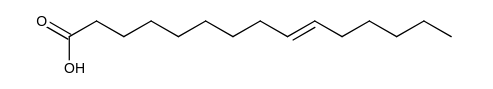
\includegraphics{smile-da75591c7049efa93e1a06be2193f4e0ca1c522e}\\
B.\\
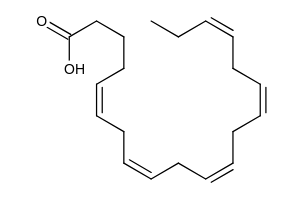
\includegraphics{smile-0b21e89fba5e44449c427b77a4680ba4b66c4433}\\
C.\\
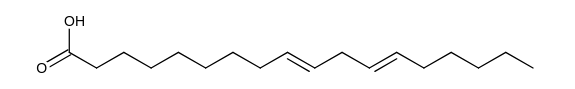
\includegraphics{smile-266becb2a8e1358891aec4a5d849a31b0daf609e}\\
D.\\
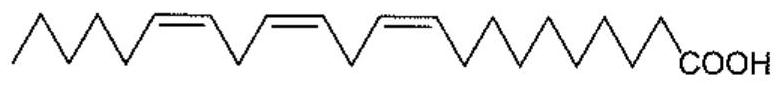
\includegraphics[max width=\textwidth, center]{2025_10_23_74efce88ce3a451fd6b0g-003}

\section*{Hãy chọn đúng hoặc sai cho mỗi ý $\mathrm{a}, \mathrm{b}, \mathrm{c}, \mathrm{d}$ ở các câu $1.20-1.22$.}
1.20. a) Một số ester có mùi thơm, không độc, được dùng làm hương liệu trong công nghiệp thực phẩm, mĩ phẩm,...\\
b) Ester thường ít tan trong nước và nhẹ hơn nước.\\
c) Phản ứng xà phòng hoá ethyl acetate là phản ứng thuận nghịch.\\
d) Trong phản ứng ester hoá giữa carboxylic acid và alcohol, nước tạo thành từ -OH trong nhóm -COOH của acid và H trong nhóm -OH của alcohol.\\
1.21. a) Các chất béo thường không tan trong nước và nhẹ hơn nước.\\
b) Chất béo là triester của glycerol với các acid đơn chức.\\
c) Cho dầu ăn vào nước, lắc đều, sau đó thu được dung dịch đồng nhất.\\
d) Phản ứng hydrogen hoá chất béo dùng để chuyển gốc acid béo không no thành gốc acid béo no.\\
1.22. a) Các acid béo là acid hữu cơ, có công thức chung là RCOOH trong đó R là hydrogen hoặc gốc hydrocarbon.\\
b) Phản ứng thuỷ phân ester trong môi trường acid là phản ứng thuận nghịch.\\
c) Bơ nhân tạo được điều chế bằng phản ứng hydrogen hoá chất béo có trong mỡ động vật.\\
d) Các chất béo dạng rắn ở nhiệt độ phòng chứa chủ yếu các gốc acid béo no.\\
1.23. Xà phòng hoá hoần toàn $4,4 \mathrm{~g}$ ethyl acetate bằng dung dịch NaOH dư, thu được bao nhiêu gam muối sodium acetate?

\section*{VAN DUNG}
1.24. Thực hiện phản ứng ester hoá sau: cho $0,1 \mathrm{~mol}$ alcohol tác dụng với $0,1 \mathrm{~mol}$ carboxylic acid, có mặt $\mathrm{H}_{2} \mathrm{SO}_{4}$ đặc làm xúc tác.\\
Đồ thị nào sau đây biểu diễn sự thay đổi số mol (n) alcohol theo thời gian (t)?

\begin{figure}[h]
\begin{center}
  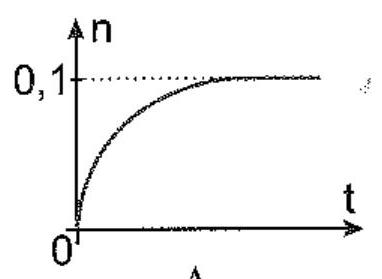
\includegraphics[width=\textwidth]{2025_10_23_74efce88ce3a451fd6b0g-004}
\captionsetup{labelformat=empty}
\caption{A}
\end{center}
\end{figure}

\begin{figure}[h]
\begin{center}
  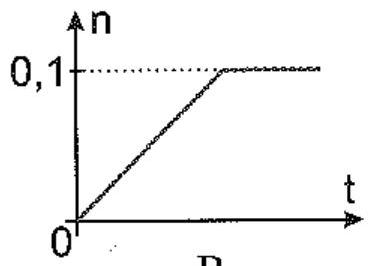
\includegraphics[width=\textwidth]{2025_10_23_74efce88ce3a451fd6b0g-004(2)}
\captionsetup{labelformat=empty}
\caption{B}
\end{center}
\end{figure}

\begin{figure}[h]
\begin{center}
  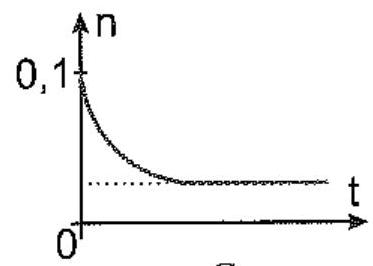
\includegraphics[width=\textwidth]{2025_10_23_74efce88ce3a451fd6b0g-004(1)}
\captionsetup{labelformat=empty}
\caption{C}
\end{center}
\end{figure}

\begin{center}
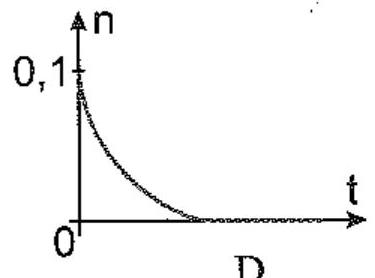
\includegraphics[max width=\textwidth]{2025_10_23_74efce88ce3a451fd6b0g-004(3)}
\end{center}

\section*{Hãy chọn đúng hoặc sai cho mỗi ý a, b, c, d ở các câu 1.25-1.26.}
1.25. Methyl butanoate là ester có mùi táo, thu được khi cho butanoic acid tác dụng với methyl alcohol có mặt $\mathrm{H}_{2} \mathrm{SO}_{4}$ đặc làm xúc tác.\\
a) Phản ứng điều chế ester ở trên là phản ứng thuận nghịch.\\
b) Phản ứng trên có tên gọi là phản ứng xà phòng hoá.\\
c) Hiệu suất phản ứng có thể đạt tối đa là $100 \%$.\\
d) Khi hệ đạt tới trạng thái cân bằng, nếu thêm nước thì lượng ester thu được sẽ tăng lên.\\
1.26. Sử dụng Hình 1.2 SGK (trang 10).\\
a) Dầu thực vật thường có hàm lượng gốc acid béo no thấp hơn mỡ động vật.\\
b) Mỡ lợn có nhiệt độ nóng chảy thấp hơn mỡ bò.\\
c) Số liên kết đôi trong gốc acid béo của dầu oliu nhiều hơn dầu hướng dương.\\
d) Khi thực hiện phản ứng hydrogen hoá dầu đậu nành và dầu oliu để tạo bơ thực vật, dầu oliu cần lượng hydrogen nhiều hơn.\\
1.27. Cho $0,1 \mathrm{~mol}$ butanoic acid tác dụng với $0,1 \mathrm{~mol}$ methyl alcohol có mặt $\mathrm{H}_{2} \mathrm{SO}_{4}$ đặc làm xúc tác. Tính khối lượng ester tạo thành. (Giả thiết $67 \%$ alcohol chuyển hoá thành ester).\\
1.28. Số miligam KOH dùng để xà phòng hoá hết lượng triglycerid có trong 1 g chất béo được gọi là chỉ số ester hoá của loại chất béo đó. Tính chỉ số ester của một loại chất béo chứa $65 \%$ tristearin và $23 \%$ triolein.\\
1.29. Dầu hạt hướng dương có thể được sử dụng để làm bơ thực vật bằng phản ứng hydrogen hoá. Triacylglycerol trong dầu hạt hướng dương chứa hai gốc linoleate và một gốc oleate.\\
a) Viết công thức cấu tạo thu gọn của các đồng phân triacylglycerol có trong dầu hạt hướng dương.\\
b) Chất béo được tiêu hoá trong cơ thể qua phản ứng thuỷ phân với xúc tác enzyme lipase, tạo glycerol và acid béo tương ứng. Sử dụng một trong các đồng phân, viết phương trình hoá học của phản ứng thuỷ phân dầu hướng dương trong quá trình tiêu hoá.\\
c) Sử dụng một trong các đồng phân, viết phương trình hoá học của phản ứng xảy ra khi hydrogen hoá hoàn toàn dầu hướng dương để làm bơ thực vật.

\section*{BÀI 2}
\section*{XÀ PHÒNG VÀ CHẤT GIẠT RỪA}
\section*{NHAN BIÉT}
2.1. Xà phòng và chất giặt rửa có đặc điểm chung nào sau đây?\\
A. Không tan trong nước.\\
B. Là muối sodium hoặc potassium của acid béo.\\
C. Là muối sulfonate hoặc sulfate của acid béo.\\
D. Thường có cấu tạo gồm hai phần là phần không phân cực (kị nước) và phần phân cực (ưa nước).\\
2.2. Chất nào sau đây được sử dụng làm xà phòng?\\
A. $\mathrm{CH}_{3} \mathrm{COOK}$.\\
B. $\mathrm{C}_{15} \mathrm{H}_{31} \mathrm{COONa}$.\\
C. $\mathrm{CH}_{3}\left[\mathrm{CH}_{2}\right]_{11} \mathrm{OSO}_{3} \mathrm{Na}$.\\
D. $\mathrm{C}_{15} \mathrm{H}_{31} \mathrm{COOCH}_{3}$.\\
2.3. Dung dịch nào sau đây là chất giặt rửa tự nhiên?\\
A. Nước quả cam.\\
B. Nước quả chanh.\\
C. Nước quả bồ kết.\\
D. Nước quá dâu.\\
2.4. Sản phẩm của phản ứng nào sau đây dùng để sản xuất xà phòng?\\
A. Thuỷ phân tinh bột.\\
B. Thuỷ phân ester có mạch carbon ngắn (< 12 C ) bằng dung dịch NaOH .\\
C. Thuỷ phân dầu thực vật hoặc mỡ động vật bằng dung dịch NaOH .\\
D. Thử phân dầu thực vật hoặc mỡ động vật trong môi trường acid.\\
2.5. Thuỷ phân hoàn toàn triglyceride X bằng dung dịch NaOH thu được xà phòng có công thức là $\mathrm{C}_{17} \mathrm{H}_{35} \mathrm{COONa}$. Công thức cấu tạo của X là\\
A. $\left(\mathrm{C}_{17} \mathrm{H}_{35} \mathrm{COO}\right)_{3} \mathrm{C}_{3} \mathrm{H}_{5}$.\\
B. $\left(\mathrm{C}_{17} \mathrm{H}_{33} \mathrm{COO}\right)_{3} \mathrm{C}_{3} \mathrm{H}_{5}$.\\
C. $\mathrm{C}_{17} \mathrm{H}_{35} \mathrm{COOC}_{3} \mathrm{H}_{5}$.\\
D. $\left(\mathrm{C}_{15} \mathrm{H}_{31} \mathrm{COO}\right)_{3} \mathrm{C}_{3} \mathrm{H}_{5}$.\\
2.6. Chất giặt rửa tổng hợp chủ yếu được sản xuất từ\\
A. mỡ động vật.\\
B. dầu thực vật.\\
C. quả bồ kết, bồ hòn.\\
D. dầu mỏ.

\section*{THONG HISU}
2.7. Khi cho vài giột dầu ăn vào dung dịch xà phòng, lắc đều. Hiện tượng quan sát được là\\
A. dầu ăn không tan và nổi lên trên.\\
B. dầu ăn không tan và chìm xuống dưới.\\
C. dầu ăn tan vào dung dịch xà phòng.\\
D. dầu ăn kết tủa lắng xuống dưới đáy.\\
2.8. Hợp chất nào sau đây được sử dụng làm chất giặt rửa tổng hợp?\\
A. $\mathrm{CH}_{3} \mathrm{COONa}$.\\
B. $\mathrm{CH}_{3}\left[\mathrm{CH}_{2}\right]_{12} \mathrm{COONa}$.\\
C. $\mathrm{CH}_{3}\left[\mathrm{CH}_{2}\right]_{12} \mathrm{COOCH}_{3}$.\\
D. $\mathrm{CH}_{3}\left[\mathrm{CH}_{2}\right]_{11} \mathrm{OSO}_{3} \mathrm{Na}$.\\
2.9. Không nên dùng xà phòng khi giặt rửa với nước cứng vì\\
A. cần dùng lượng nước nhiều hơn.\\
B. gây ô nhiễm môi trường.\\
C. ion $\mathrm{Ca}^{2+}, \mathrm{Mg}^{2+}$ làm giảm độ bền sợi vải.\\
D. xuất hiện kết tủa làm giảm tác dụng giặt rửa của xà phòng.\\
2.10. Khi xà phòng hoá triglycerid X bằng dung dịch NaOH dư, đun nóng, thu được xà phòng gồm hỗn hợp ba muối sodium oleate, sodium stearate và sodium palmitate. Số đồng phân cấu tạo có thể có của X là\\
A. 2 .\\
B. 1 .\\
C. 3 .\\
D. 4 .

\section*{Hãy chọn đúng hoăc sai cho mỗi ý $\mathrm{a}, \mathrm{b}, \mathrm{c}, \mathrm{d}$ ở các câu 2.11-2.12.}
2.11. a) Xà phòng và chất giặt rưa thường có cấu tạo gồm hai phần: ưa nước và kị nước.\\
b) Xà phòng hoá tripalmitin với dung dịch NaOH thu được sản phẩm là $\mathrm{C}_{15} \mathrm{H}_{29} \mathrm{COONa}$ và glycerol.\\
c) Chất giặt rưa tổng hợp thường được điều chế từ chất béo.\\
d) Mỡ động vật, dầu thực vật là nguyên liệu để sản xuất xà phòng.\\
2.12. a) Chất giặt rửa thường là muối sodium alkylsulfate hoặc alkylbenzene sulfonate.\\
b) Phân tử chất giặt rưa gồm một đầu kị nước gắn với một đầu ưa nước.\\
c) Khi giặt rửa bằng nước cứng nên sử dụng xà phòng.\\
d) Phản ứng thuỷ phân chất béo trong môi trường kiềm $(\mathrm{NaOH}, \mathrm{KOH})$ thuộc loại phản ứng xà phòng hoá.

\section*{VAN DUNG}
2.13. Thông thường, nếu mạch carbon của chất giặt rửa tổng hợp không phân nhánh thì chất tẩy rửa đó dễ phân huỷ sinh học hơn so với mạch carbon phân nhánh. Chất tẩy rửa nào sau đây thân thiện với môi trường nhất?\\
A.\\
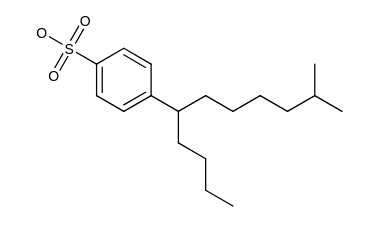
\includegraphics{smile-2e5e834685bbef91efaf354f3233b12c3a1ab74d}\\
B.\\
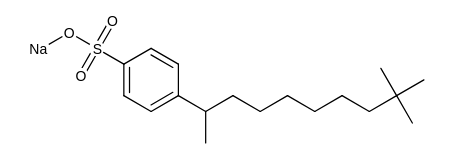
\includegraphics{smile-ecacd046a34735305dab26b5868c3eb593ab2f2f}\\
C.\\
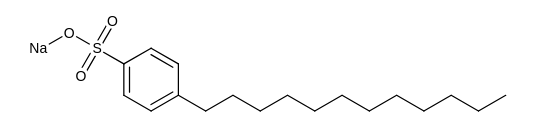
\includegraphics{smile-2b6ebd6daa642cf6773f02712e7f59cbacbf6870}\\
D.\\
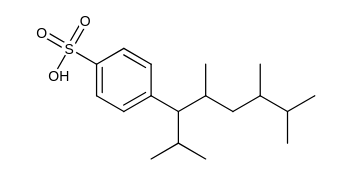
\includegraphics{smile-c64e3fcf51cc461cf6f35353faa7c225cdbebf3a}

\section*{Hãy chọn đúng hoăc sai cho mổi ý $\mathfrak{a}, \mathfrak{b}, \mathfrak{c}, \mathfrak{d}$ ở các câu 2.14-2.15.}
2.14. a) Chất kị nước là những chất không tan trong dầu mỡ, hydrocarbon,...\\
b) Muối sodium hoặc potassium của carboxylic acid được dùng làm xà phòng.\\
c) Xà phòng bị giảm hoặc mât tác dụng tẩy rửa khi dùng nước cứng vì gốc acid béo dễ kết tủa với cation $\mathrm{Ca}^{2+}, \mathrm{Mg}^{2+}$.\\
d) Xà phòng, chất giặt rửa tan vào nước tạo dung dịch có sức căng bề mặt nhỏ làm cho vật cần giặt rửa dễ thấm ướt.\\
2.15. Có bốn ống nghiệm: ống (1) chứa 3 mL nước cất; ống (2) chứa 3 mL nước xà phòng; ống (3) chứa 3 mL nước xà phòng và 3 giọt dung dịch $\mathrm{CaCl}_{2}$ bão hoà; ống (4) chứa 3 mL nước giặt rửa tổng hợp và 3 giọt dung dịch $\mathrm{CaCl}_{2}$ bão hoà. Cho vào mỗi ống nghiệm 3 giọt dầu ăn, lắc đều.\\
a) Trong ống nghiệm (1), dầu ăn không tan và chìm xuống dưới.\\
b) Trong ống nghiệm (2), dầu ăn tan tạo hỗn hợp đồng nhất.\\
c) Trong ống nghiệm (3) có kết tủa xuất hiện.\\
d) Trong ống nghiệm (4), dầu ăn tan tạo hỗn hợp đồng nhất.\\
2.16. Đường ống thoát nước của bồn rửa chén bát sau khi sử dụng một thời gian có thể bị tắc do chất béo dạng rắn (như glyceryl tristearate (tristearin) có trong mỡ động vật) đọng ở trong đường ống. Để thông tắc, có thể cho một ít NaOH dạng rắn vào đường ống thoát nước.\\
a) Giải thích hiện tượng và viết phương trình hoá học của phản ứng xảy ra trong quá trình thông tắc.\\
b) Nếu dừng 12 g NaOH rắn thì có thể xà phòng hoá tối đa được bao nhiêu gam tristearin?\\
2.17. Chỉ số xà phòng hoá là số miligam KOH dùng để xà phòng hoá hết triglycerid và trung hoà hết lượng acid tự do trong 1 g chất béo. Một chất béo chứa $3,55 \%$ stearic acid và $89 \%$ tristearin về khối lượng, còn lại là các chất không tham gia phản ứng với KOH . Tính chỉ số xà phòng hoá của chất béo trên.

\section*{BÀI 3}
\section*{ÔN TÂP CHƯƠNG I}
\section*{NHAN BIET}
3.1. Chất nào sau đây thuộc loại ester?\\
A. $\mathrm{HCOOCH}_{3}$.\\
B. $\mathrm{CH}_{3} \mathrm{COOH}$.\\
C. HCOOH .\\
D. $\mathrm{CH}_{3} \mathrm{COCH}_{3}$.\\
3.2. Số đồng phân cấu tạo của ester có công thức $\mathrm{C}_{4} \mathrm{H}_{8} \mathrm{O}_{2}$ là\\
A. 2 .\\
B. 3 .\\
C. 4 .\\
D. 5 .\\
3.3. Ester được tạo bởi ethanol và formic acid có công thức cấu tạo là\\
A. $\mathrm{HCOOCH}_{3}$.\\
B. $\mathrm{CH}_{3} \mathrm{COOC}_{2} \mathrm{H}_{5}$.\\
C. $\mathrm{HCOOC}_{2} \mathrm{H}_{5}$.\\
D. $\mathrm{CH}_{3} \mathrm{COOCH}_{3}$.\\
3.4. Acid nào sau đây thuộc loại acid béo?\\
A. HCOOH .\\
B. $\mathrm{CH}_{3} \mathrm{COOH}$.\\
C. $\mathrm{C}_{2} \mathrm{H}_{5} \mathrm{COOH}$.\\
D. $\mathrm{C}_{17} \mathrm{H}_{31} \mathrm{COOH}$.\\
3.5. Chất nào sau đây thường được dùng làm xúc tác cho phản ứng điều chế ester từ carboxylic acid và alcohol?\\
A. Hydrochloric acid.\\
B. Sulfuric acid.\\
C. Sulfurous acid.\\
D. Nitric acid.\\
3.6. Thuỷ phân methyl propanoate trong môi trường acid thu được sản phẩm gồm:\\
A. $\mathrm{CH}_{3} \mathrm{COOH}$ và $\mathrm{C}_{3} \mathrm{H}_{7} \mathrm{OH}$.\\
B. $\mathrm{CH}_{3} \mathrm{COOH}$ và $\mathrm{C}_{2} \mathrm{H}_{5} \mathrm{OH}$.\\
C. $\mathrm{C}_{2} \mathrm{H}_{5} \mathrm{COOH}$ và $\mathrm{C}_{2} \mathrm{H}_{5} \mathrm{OH}$.\\
D. $\mathrm{C}_{2} \mathrm{H}_{5} \mathrm{COOH}$ và $\mathrm{CH}_{3} \mathrm{OH}$.\\
3.7. Chất nào sau đây là thành phần chính của xà phòng?\\
A. $\mathrm{C}_{6} \mathrm{H}_{5} \mathrm{COONa}$.\\
B. $\mathrm{C}_{17} \mathrm{H}_{35} \mathrm{COONa}$.\\
C. $\mathrm{CH}_{3}\left[\mathrm{CH}_{2}\right]_{11} \mathrm{OSO}_{3} \mathrm{Na}$.\\
D. $\mathrm{CH}_{3}\left[\mathrm{CH}_{2}\right]_{11} \mathrm{SO}_{3} \mathrm{Na}$.\\
3.8. Ethyl propanoate là ester tạo nên mùi thơm đặc trưng của quả dứa. Công thức của ethyl propanoate là\\
A. $\mathrm{CH}_{3} \mathrm{COOC}_{2} \mathrm{H}_{5}$.\\
B. $\mathrm{C}_{2} \mathrm{H}_{5} \mathrm{COOCH}_{2} \mathrm{CH}_{2} \mathrm{CH}_{3}$.\\
C. $\mathrm{CH}_{3} \mathrm{COOCH}_{2} \mathrm{CH}_{2} \mathrm{CH}_{3}$.\\
D. $\mathrm{C}_{2} \mathrm{H}_{5} \mathrm{COOC}_{2} \mathrm{H}_{5}$.\\
3.9. Công thức cấu tạo nào sau đây là của chất béo glyceryl trioleate (triolein)?\\
A. $\left(\mathrm{C}_{17} \mathrm{H}_{35} \mathrm{COO}\right)_{3} \mathrm{C}_{3} \mathrm{H}_{5}$.\\
B. $\left(\mathrm{C}_{17} \mathrm{H}_{33} \mathrm{COO}\right)_{3} \mathrm{C}_{3} \mathrm{H}_{5}$.\\
C. $\left(\mathrm{C}_{17} \mathrm{H}_{31} \mathrm{COO}\right)_{3} \mathrm{C}_{3} \mathrm{H}_{5}$.\\
D. $\left(\mathrm{C}_{16} \mathrm{H}_{33} \mathrm{COO}\right)_{3} \mathrm{C}_{3} \mathrm{H}_{5}$.

\section*{THONG MIU}
3.10. Quần áo bị dính bẩn bởi dầu luyn (dầu nhớt). Nên sử dụng chất nào sau đây để loại bỏ vết bẩn đó?\\
A. Dung dịch muối ăn.\\
B. Chất giặt rửa tổng hợp.\\
C. Dung dịch HCl .\\
D. Dung dịch NaOH .

Hãy chọn đúng hoặc sai cho mỗi ý $a, b, c, d$ ở các câu 3.11-3.12.\\
3.11. a) Acid béo thường có gốc hydrocarbon mạch dài, có số nguyên tử carbon lẻ.\\
b) Khi xà phòng hoá chất béo, sản phẩm thu được là glycerol và các acid đơn chức.\\
c) Chất béo có nhiều gốc acid no thường ở dạng rắn, còn chất béo có nhiều gốc acid không no thường ở dạng lỏng.\\
d) Acid béo omega-3 là các acid béo không no có liên kết đôi đầu tiên ở vị trí số 3 nếu đánh số từ nhóm carboxyl ( -COOH ).\\
3.12. a) Xà phòng và chất giặt rửa tổng hợp đều có phần kị nước là gốc hydrocarbon mạch dài.\\
b) Xà phòng là muối của carboxylic acid với sodium, potassium.\\
c) Một số chất giặt rửa tổng hợp khó phân huỷ sinh học.\\
d) Khi giặt quần áo bằng nước cứng nên sử dụng chất giặt rửa tổng hợp.\\
3.13. Thực hiện phản ứng xà phòng hoá 100 kg chất béo chứa $80 \%$ tristearin, còn lại là các tạp chất không phản ứng, thu được bao nhiêu kilogam sodium stearate? (Biết hiệu suất phản ứng xà phòng hoá là $90 \%$.)\\
3.14. Dầu mỡ khi chiên rán nhiều lần thường có mùi khó chịu do nguyên nhân chính là dầu mỡ bị\\
A. thuý phân.\\
B. xà phòng hoá.\\
C. oxi hoá.\\
D. hydrogen hoá.\\
3.15. Xà phòng hoá chất béo nào sau đây thu được sodium stearate?\\
A. $\left(\mathrm{C}_{17} \mathrm{H}_{35} \mathrm{COO}\right)_{3} \mathrm{C}_{3} \mathrm{H}_{5}$.\\
B. $\left(\mathrm{C}_{17} \mathrm{H}_{33} \mathrm{COO}\right)_{3} \mathrm{C}_{3} \mathrm{H}_{5}$.\\
C. $\left(\mathrm{C}_{17} \mathrm{H}_{31} \mathrm{COO}\right)_{3} \mathrm{C}_{3} \mathrm{H}_{5}$.\\
D. $\left(\mathrm{C}_{16} \mathrm{H}_{33} \mathrm{COO}\right)_{3} \mathrm{C}_{3} \mathrm{H}_{5}$.\\
3.16. Cho vào ba ống nghiệm, mỗi ống 1 mL ethyl acetate, sau đó cho vào mỗi ống các chất sau:

\begin{itemize}
  \item Ống nghiệm (1): 2 mL nước cất.
  \item Ống nghiệm (2): 2 mL dung dịch $\mathrm{H}_{2} \mathrm{SO}_{4} 20 \%$.\\
-Ống nghiệm (3): 2 mL dung dịch $\mathrm{NaOH} 30 \%$.\\
Lắc đều ba ống nghiệm rồi đặt ba ống trong nồi cách thuỷ ở nhiệt độ $60-70^{\circ} \mathrm{C}$. Sau một thời gian, thể tích lớp ester còn lại trong ba ống theo thứ tự giảm dần là:\\
A. $(3)>(2)>(1)$.\\
B. $(2)>(3)>(1)$.\\
C. $(1)>(2)>(3)$.\\
D. (1) $>$ (3) $>$ (2).\\
3.17. Xà phòng hoá hoàn toàn $4,42 \mathrm{~g}$ triglyceride X bằng dung dịch NaOH dư, sau phản ứng thu được m gam hỗn hợp các muối sodium linoleate, sodium oleate và sodium stearate. Hydrogen hoá hoàn toàn X cần dùng n lít khí hydrogen ở điều kiện chuẩn. Tính giá trị $\mathrm{m}, \mathrm{n}$.\\
3.18. Một loại dầu thực vật trong đó thành phần chất béo chứa hai gốc linoleate, một gốc oleate và thành phần phần trăm khối lượng chất béo trong dầu thực vật là $88 \%$. Tính chỉ số ester ${ }^{(1)}$ của dầu thực vật đó.\\
3.19. Tổng số kilocalo (kcal) và tổng số gam chất béo trong một số thức ăn nhanh được liệt kê ở bảng dưới đây.
\end{itemize}

\begin{center}
\begin{tabular}{|l|l|l|}
\hline
Thire an nhanh (suát) & Tong nang lurgng (kcal) & Tóng só chát béo (g) \\
\hline
Thịt gà chiên rán & 830 & 46 \\
\hline
Bánh mì kẹp phô mai & 520 & 29 \\
\hline
Bánh mì kẹp hamburger & 254 & 7 \\
\hline
Bánh pizza & 560 & 18 \\
\hline
Khoai tây chiên & 279 & 13 \\
\hline
Một chiếc xúc xích cỡ lớn & 180 & 18 \\
\hline
\end{tabular}
\end{center}

a) Tính lượng kcal được cung cấp từ chất béo trong mỗi loại thức ăn nhanh, làm tròn kết quả đến hàng đơn vị. (Biết rằng 1 g chất béo giải phóng 9 kcal .)\\
b) Trong các loại thức ăn đó, thức ăn nào có tỉ lệ \% chất béo đóng góp nhiều nhất vào tổng năng lượng của thức ăn.\\
c) Trong các thức ăn trên, thức ăn nào có nguy cơ gây béo phì biết rằng chế độ ăn uống phù hợp để tránh béo phì, chất béo nên chiếm $20 \%-35 \%$ tổng năng lượng cung cấp từ thức ăn.

\footnotetext{(1) Chỉ số ester; xem bài 1.28 trang 9 .
}\section*{Chuong II CARBOHYDRATE}
\section*{BÀl 4}
\section*{GIÓI THIỆU VỀ CARBOHYDRATE. GLUCOSE VÀ FRUCTOSE}
\section*{NHAN BIET}
4.1. Carbohydrate là hợp chất hữu cơ\\
A. chứa đồng thời nhóm amino và nhóm carboxyl.\\
B. chữa đồng thời nhóm hydroxy và nhóm carboxyl.\\
C. tạp chức, thường có công thức chung là $\mathrm{C}_{\mathrm{n}}\left(\mathrm{H}_{2} \mathrm{O}\right)_{\mathrm{m}}$.\\
D. đa chức, chứa nhiều nhóm hydroxy liên tiếp.\\
4.2. Glucose và fructose thuộc loại carbohydrate nào sau đây?\\
A. Monosaccharide.\\
B. Disaccharide.\\
C. Polysaccharide.\\
D. Oligosaccharide.\\
4.3. Công thức phân tử chung của glucose và fructose là\\
A. $\mathrm{C}_{6} \mathrm{H}_{10} \mathrm{O}_{5}$.\\
B. $\mathrm{C}_{6} \mathrm{H}_{12} \mathrm{O}_{6}$.\\
C. $\mathrm{C}_{5} \mathrm{H}_{10} \mathrm{O}_{5}$.\\
D. $\mathrm{C}_{12} \mathrm{H}_{22} \mathrm{O}_{11}$.\\
4.4. Nhóm chức nào sau đây không có trong cấu tạo của glucose?\\
A. Aldehyde.\\
B. Hydroxy.\\
C. Ketone.\\
D. Hemiacetal.\\
4.5. Fructose có bao nhiêu nhóm hydroxy trong cấu tạo?\\
A. 3 .\\
B. 4 .\\
C. 5.\\
D. 6 .\\
4.6. Glucose và fructose không có điểm chung nào sau đây?\\
A. Dễ tan trong nước.\\
B. Có vị ngọt.\\
C. Chất rắn ở điều kiện thường.\\
D. Hình thành trực tiếp từ quá trình quang hợp.\\
4.7. Dung dịch glucose không có tính chất hoá học nào sau đây?\\
A. Phản ứng với $\mathrm{Cu}(\mathrm{OH})_{2}$.\\
B. Phản ứng với thuốc thử Tollens.\\
C. Phản ứng với nước bromine.\\
D. Phản ứng thuỷ phân.\\
4.8. Chất nào sau đây có thể điểu chế từ glucose qua quá trình lên men?\\
A. Ethanol.\\
B. Lactic acid.\\
C. Methane.\\
D. Fructose.\\
4.9. Trong môi trường kiềm, glucose và fructose có thể chuyển hoá lẫn nhau. Điều đó chứng tỏ hai chất này\\
A. đều phản ứng với thuốc thử Tollens.\\
B. đều là những disaccharide.\\
C. đều làm mất màu nước bromine.\\
D. đều không có nhóm hydroxy.\\
4.10. Glucose quan trọng đối với cơ thể sống vì nó\\
A. là nguiồn cung cấp nước và carbon dioxide.\\
B. cung cấp năng lượng cho quá trình sinh hoá tế bào.\\
C. xúc tác cho các quá trình sinh hoá.\\
D. làm giảm quá trình oxi hoá của gốc tự do.

\section*{THONG HILU}
Hãy chọn đúng hoặc sai cho mỗi ý $a, b, c, d$ ở các câu $4.11-4.15$.\\
4.11. a) Glucose và fructose là những đường không thể bị thuỷ phân.\\
b) Fructose có cấu tạo hoá học hoàn toàn giống với glucose.\\
c) Saccharose và maltose là những disaccharide.\\
d) Tinh bột và cellulose là những polysaccharide.\\
4.12. a) Glucose và fructose đều có công thức phân tử là $\mathrm{C}_{6} \mathrm{H}_{12} \mathrm{O}_{6}$.\\
b) Glucose và fructose đều tồn tại dạng mạch hở và mạch vòng.\\
c) Glucose và fructose đều là pentahydroxy aldehyde.\\
d) Dạng vòng của glucose và fructose đều là vòng sáu cạnh.\\
4.13. a) Tất cả các loại carbohydrate đều tan hoàn toàn trong nước.\\
b) Một số đường đơn (monosaccharide) có vị ngọt.\\
c) Carbohydrate chỉ được tìm thấy trong thực phẩm có nguồn gốc thực vật.\\
d) Glucose và fructose đều là chất rắn, vị ngọt, tan tốt trong nước.\\
4.14. Phát biểu về tính chất hoá học của glucose và fructose:\\
a) Đều phản ứng được với thuốc thử Tollens.\\
b) Đều làm mất màu nước bromine.\\
c) Dung dịch mỗi chất đều hoà tan được $\mathrm{Cu}(\mathrm{OH})_{2}$.\\
d) Đều phản ứng được với $\mathrm{Cu}(\mathrm{OH})_{2}$ trong kiềm nóng tạo kết tủa đỏ gạch.\\
4.15. a) Fructose phản ứng với thuốc thử Tollens sinh ra ammonium gluconate.\\
b) Glucose phản ứng với $\mathrm{Cu}(\mathrm{OH})_{2}$ trong dung dịch NaOH nóng tạo sodium gluconate.\\
c) Glucose phản ứng với nước bromine tạo gluconic acid.\\
d) Lên men rượu glucose sinh ra ethanol và carbon dioxide.\\
4.16. Điểm khác biệt cơ bản về cấu tạo của glucose và fructose là gì?\\
4.17. Giới thiệu một số loại thực phẩm tự nhiên giàu glucose và một số loại thực phẩm tự nhiên giàu fructose.\\
4.18. Một mẫu nước cam có khối lượng riêng $1,05 \mathrm{~g} / \mathrm{mL}$, chứa $2,5 \%$ fructose và $2,0 \%$ glucose về khối lượng. Tính khối lượng mỗi loại đường này trong 250 mL mẫu nước cam trên.\\
4.19. Nêu một ứng dụng dựa trên phản ứng lên men rượu của glucose.

\section*{VAN DUNG}
4.20. Methyl $\alpha$-glucoside và methyl $\beta$-glucoside có tham gia phản ứng với thuốc thử Tollens không? Tại sao?\\
4.21. Tại sao glucose lại được coi là nguồn năng lượng chính cho các tế bào trong cơ thể?\\
4.22. Trình bày ứng dụng của glucose trong lĩnh vực y tế và thể thao.\\
4.23. Một nhóm học sinh muốn thử nghiệm phản ứng tráng bạc lên kính bằng nguyên liệu đầu là glucose. Giả sử lớp bạc có diện tích là $100 \mathrm{~cm}^{2}$ và độ dày là $0,5 \mu \mathrm{~m}$. Biết rằng khối lượng riêng của bạc là $10,49 \mathrm{~g} / \mathrm{cm}^{3}$ và khối lượng mol\\
của glucose là $180 \mathrm{~g} / \mathrm{mol}$. Tính lượng glucose cần dùng với giả thiết hiệu suất phản ứng là $100 \%$.\\
4.24. Một nhà máy sản xuất rượu vang sử dụng 500 kg nho cho một mẻ lên men. Tính khối lượng ethanol thu được. (Giả thiết hiệu suất phản ứng lên men đạt $100 \%$, trong mỗi kg nho chứa 200 g glucose.)

\section*{BÀI 5}
\section*{SACCHAROSE VÀ MALTOSE}
\section*{NHAN BIET}
5.1. Saccharose được cấu tạo từ\\
A. hai đơn vị glucose qua liên kết $\alpha-1,4$-glycoside.\\
B. một đơn vị glucose và một đơn vị fructose qua liên kết $\alpha-1,2$-glycoside.\\
C. hai đơn vị fructose qua liên kết $\beta$ - 1,4 -glycoside.\\
D. một đơn vị glucose và một đơn vị galactose qua liên kết $\alpha-1,4-$ glycoside.\\
5.2. Maltose được tạo ra từ quá trình nào sau đây?\\
A. Thuỷ phân saccharose.\\
B. Thuỷ phân tinh bột.\\
C. Kết hợp glucose và fructose.\\
D. Lên men ethanol.\\
5.3. Saccharose tham gia phản ứng nào sau đây?\\
A. Phản ứng với thuốc thử Tollens.\\
B. Phản ứng với nước bromine.\\
C. Phản ứng với $\mathrm{Cu}(\mathrm{OH})_{2}$ tạo dung dịch màu xanh lam.\\
D. Phản ứng thuỷ phân trong môi trường kiềm.\\
5.4. Phản ứng đặc trưng của maltose là\\
A. phản ứng với dung dịch NaOH .\\
B. phản ứng màu với iodine.\\
C. phản ứng thuỷ phân tạo ra glucose.\\
D. phản ứng lên men trực tiếp tạo ra ethanol.\\
5.5. Saccharose và maltose đều tham gia phản ứng nào sau đây?\\
A. Phản ứng với thuốc thử Tollens.\\
B. Phản ứng thuỷ phân trong môi trường acid.\\
C. Phản ứng với dung dịch nước bromine.\\
D. Phản ứng với $\mathrm{Cu}(\mathrm{OH})_{2}$ tạo kết tủa đỏ gạch.\\
5.6. Saccharose thường được tìm thấy trong loại thực vật nào sau đây?\\
A. Cây đậu nành.\\
B. Cây lúa mì.\\
C. Cây mía.\\
D. Cây cà phê.

\section*{THONG HILU}
Hãy chọn đúng hoặc sai cho mỗi ý $\mathrm{a}, \mathrm{b}, \mathrm{c}, \mathrm{d}$ ở các câu 5.7-5.9.\\
5.7. Các phát biểu về cấu tạo của saccharose và maltose:\\
a) Maltose được tạo thành từ hai đơn vị fructose.\\
b) Maltose có liên kết $\alpha-1,4$-glycoside giữa hai đơn vị glucose.\\
c) Phân tử saccharose chứa một liên kết $\beta$-1,2-glycoside.\\
d) Phân tử saccharose chỉ tồn tại dạng mạch vòng.\\
5.8. Các phát biểu về tính chất của saccharose và maltose:\\
a) Saccharose không thể tạo dung dịch màu xanh lam khi phản ứng với $\mathrm{Cu}(\mathrm{OH})_{2}$.\\
b) Saccharose không phản ứng với thuốc thử Tollens.\\
c) Saccharose có thể bị thuỷ phân thành glucose và fructose.\\
d) Maltose có thể phản ứng với thuốc thử Tollens và làm mất màu nước bromine.\\
5.9. Các phát biểu về trạng thái tự nhiên và ứng dụng của saccharose và maltose:\\
a) Saccharose và maltose thường được sử dụng trong sản xuất bánh kẹo.\\
b) Saccharose là nguồn cung cấp năng lượng quan trọng cho con người.\\
c) Saccharose có nhiều trong cây mía, củ cải đường và hoa thốt nốt.\\
d) Maltose có trong một số hạt nảy mầm từ quá trình thuỷ phân tinh bột.\\
5.10. Tại sao maltose có thể phản ứng với thuốc thử Tollens, dung dịch nước bromine, còn saccharose không thể tham gia các phản ứng này?\\
5.11. Tại sao khi đun nóng saccharose với dung dịch HCl thu được dung dịch phản ứng với $\mathrm{Cu}(\mathrm{OH})_{2}$ (có mặt dung dịch NaOH , đun nóng), tạo kết tủa đỏ gạch? Viết phương trình hoá học minh hoạ.

\section*{VAN DUNG}
5.12. Việc tiêu thụ maltose và saccharose trong chế độ ăn uống hằng ngày ảnh hưởng đến sức khoẻ răng miệng như thế nào?\\
5.13. Hãy tìm hiểu thông tin để đánh giá lời khuyên "Giảm tiêu thụ đường tinh luyện và sử dụng loại đường tự nhiên thay thế đường tinh luyện khi có thể".\\
5.14. Trong quá trình sản xuất bia, maltose được tạo ra từ quá trình lên men của mạch nha. Một nhà máy bia dự định sản xuất 10000 kg maltose để đáp ứng nhu cầu sản xuất bia thì nhà máy này cần nhập bao nhiêu bao mạch nha? (Biết 1 kg mạch nha có thể tạo ra $0,8 \mathrm{~kg}$ maltose, khối lượng mỗi bao là 50 kg .)

\section*{BÀI 6}
\section*{TINH BỘT VÀ CELLULOSE}
\section*{NHAN BIET}
6.1. Tinh bột chứa hỗn hợp chất nào sau đây?\\
A. Glucose và fructose.\\
B. Amylose và cellulose.\\
C. Amylose và amylopectin.\\
D. Glucose và galactose.\\
6.2. Amylopectin khác biệt cơ bản với amylose ở điểm nào sau đây?\\
A. Có cấu tạo mạch phân nhánh.\\
B. Chỉ chứa liên kết $\alpha-1,4$-glycoside.\\
C. Không tan trong nước.\\
D. Tạo màu xanh tím với iodine.\\
6.3. Phân tử cellulose cấu tạo từ các đơn vị nào sau đây?\\
A. $\alpha$-glucose.\\
B. $\beta$-glucose.\\
C. Fructose.\\
D. Galactose.\\
6.4. Tinh bột và cellulose đều tham gia phản ứng nào sau đây?\\
A. Phản ứng thuỷ phân.\\
B. Phản ứng màu với dung dịch iodine.\\
C. Phản ứng với thuốc thử Tollens.\\
D. Phản ứng với nước bromine.\\
6.5. Cellulose không tan trong nước nhưng tan trong dung dịch nào sau đây?\\
A. Dung dịch NaOH .\\
B. Dung dịch ethanol.\\
C. Nước Schweizer.\\
D. Nước bromine.\\
6.6. Cellulose phả̉n ứng với nitric acid tạo thành sản phẩm nào sau đây?\\
A. Glucose.\\
B. Dextrin.\\
C. Maltose.\\
D. Cellulose nitrate.\\
6.7. Chất nào sau đây có thể thu được khi thuỷ phân không hoàn toàn tinh bột?\\
A. Cellulose.\\
B. Dextrin.\\
C. Fructose.\\
D. Saccharose.\\
6.8. Cellulose không có tính chất nào sau đây?\\
A. Tan trong nước Schweizer.\\
B. Phản ứng tạo màu xanh tím với iodine.\\
C. Phản ứng với nitric acid tạo cellulose nitrate.\\
D. Thuỷ phân hoàn toàn tạo glucose.\\
6.9. Cellulose không được sử dụng trong ứng dụng nào sau đây?\\
A. Sản xuất các thiết bị điện.\\
B. Nguyên liệu sản xuất ethanol và cellulose nitrate.\\
C. Sản xuất giấy, tơ tự nhiên và sợi nhân tạo.\\
D. Vật liệu gỗ xây dựng.\\
6.10. Nguyên liệu nào sau đây không phải là nguồn cung cấp tinh bột?\\
A. Củ và quả.\\
B. Hạt ngũ cốc.\\
C. Sợi bông.\\
D. Gạo.

\section*{THONG HIÉU}
Hãy chọn đúng hoăc sai cho mỗi ý a, b, c, d ở các câu $6.11-6.15$.\\
6.11. a) Tinh bột và cellulose đều là polysaccharidé.\\
b) Phân tử amylose có cấu tạo không phân nhánh.\\
c) Cellulose có cấu trúc phân nhánh.\\
d) Cellulose được tạo từ các đơn vị $\beta$-glucose.\\
6.12. a) Tinh bột và cellulose đều có công thức phân tử là $\left(\mathrm{C}_{6} \mathrm{H}_{10} \mathrm{O}_{5}\right)_{n}$.\\
b) Amylopectin chứa liên kết $\alpha-1,6$-glycoside tại các điểm nhánh.\\
c) Tinh bột có trong củ, quả và hạt của thực vật.\\
d) Cellulose là thành phần chính của thành tế bào thực vật.\\
6.13. a) Tinh bột tạo màu xanh tím khi phản ứng với dung dịch iodine.\\
b) Cellulose tan tốt trong nước nóng.\\
c) Tinh bột không tan trong nước lạnh.\\
d) Cellulose không phản ứng màu với dung dịch iodine.\\
6.14. a) Cellulose có thể tạo thành cellulose nitrate khi phản ứng với $\mathrm{HNO}_{3}$.\\
b) Phản ứng thuỷ phân của cellulose tạo ra fructose.\\
c) Thuỷ phân hoàn toàn tinh bột và cellulose đều tạo thành glucose.\\
d) Cellulose tạo ra màu xanh lam khi phản ứng với nước Schweizer.\\
6.15. a) Tinh bột được sử dụng làm chất kết dính trong công nghiệp giấy.\\
b) Tinh bột là nguồn lương thực chính của con người.\\
c) Cellulose có thể được sử dụng làm nguyên liệu trong sản xuất ethanol.\\
d) Tinh bột được tiêu hoá bởi enzyme $\alpha$-amylase trong nước bọt.\\
6.16. Cellulose có thể tiêu hoá bởi enzyme trong hệ tiêu hoá của người hay không? Giải thích.\\
6.17. Tại sao cellulose là thành phần không thể thiếu trong cấu trúc tế bào thực vật.\\
6.18. Tính khối lượng glucose thu được khi thuỷ phân hoàn toàn 162 g tinh bột. (Biết hiệu suất của quá trình thuỷ phân là $80 \%$.)

\section*{VAN DUNG}
6.19. Tại sao amylopectin dễ tiêu hoá hơn amylose?\\
6.20. Tại sao bột mì có thể dùng làm chất kết dính khi nấu ăn?\\
6.21. Mô tả quá trình chuyển hoá tinh bột thành ethanol trong sản xuất nhiên liệu sinh học và vai trò của các enzyme trong quá trình 」ày.\\
6.22. Tính khối lượng ethanol có thể thu được từ 1 tấn tinh bột. (Biết hiệu suất của quá trình lên men đạt $90 \%$ ).

\section*{BÀl 7}
\section*{ÔN TẬP CHƯƠNG II}
\section*{NHAN BIET}
7.1. Carbohydrate là hợp chất hữu cơ tạp chức, thường có công thức chung là\\
A. $\left(\mathrm{C}_{\mathrm{n}} \mathrm{H}_{2}\right)_{\mathrm{m}}$.\\
B. $\mathrm{C}_{\mathrm{n}}\left(\mathrm{H}_{2} \mathrm{O}\right)_{\mathrm{m}}$.\\
C. $\mathrm{C}_{\mathrm{n}} \mathrm{H}_{2 \mathrm{n}}$.\\
D. $\mathrm{C}_{\mathrm{n}} \mathrm{H}_{2 \mathrm{n}} \mathrm{O}_{2}$.\\
7.2. Công thức phân tử của saccharose là\\
A. $\mathrm{C}_{5} \mathrm{H}_{10} \mathrm{O}_{5}$.\\
B. $\mathrm{C}_{6} \mathrm{H}_{12} \mathrm{O}_{6}$.\\
C. $\mathrm{C}_{12} \mathrm{H}_{22} \mathrm{O}_{11}$.\\
D. $\left(\mathrm{C}_{6} \mathrm{H}_{10} \mathrm{O}_{5}\right)_{\mathrm{n}}$.\\
7.3. Phát biểu nào sau đây về cấu tạo của glucose không đúng?\\
A. Có cả dạng mạch hở và mạch vòng.\\
B. Có chứa nhóm chức aldehyde.\\
C. Có chứa năm nhóm hydroxy.\\
D. Có chứa nhóm ketone.\\
7.4. Phản ứng nào sau đây không phải là tính chất của glucose?\\
A. Phản ứng với $\mathrm{Cu}(\mathrm{OH})_{2}$ tạo phức màu xanh lam.\\
B. Phản ứng với thuốc thử Tollens.\\
C. Phản ứng lên men tạo ethanol.\\
D. Phản ứng với carboxylic acid tạo ester.\\
7.5. Saccharose thuộc loại carbohydrate nào sau đây?\\
A. Monosaccharide.\\
B. Disaccharide.\\
C. Polysaccharide.\\
D. Oligosaccharide.\\
7.6. Thuỷ phân một phân tử saccharose tạo thành\\
A. hai phân tử glucose.\\
B. một phân tử glucose và một phân tử fructose.\\
C. hai phân tử fructose.\\
D. một phân tử galactose và một phân tử glucose.\\
7.7. Phản ứng đặc trưng của saccharose là\\
A. phản ứng thuỷ phân tạo glucose và fructose.\\
B. phản ứng màu với iodine.\\
C. phản ứng với $\mathrm{Cu}(\mathrm{OH})_{2}$ tạo kết tủa đỏ gạch.\\
D. phản ứng mất màu nước bromine.\\
7.8. Tinh bột và cellulose đều là\\
A. disaccharide.\\
B. monosaccharide.\\
C. polysaccharide.\\
D. oligosaccharide.\\
7.9. Phản ứng màu với dung dịch iodine là tính chất của chất nào sau đây?\\
A. Glucose.\\
B. Fructose.\\
C. Saccharose.\\
D. Tinh bột.\\
7.10. Phát biểu nào sau đây về cellulose không đúng?\\
A. Không tan trong nước.\\
B. Là nguồn nguyên liệu sản xuất giấy.\\
C. Có thể phản ứng với $\mathrm{HNO}_{3}$ tạo cellulose nitrate.\\
D. Phản ứng màu với dung dịch iodine.

\section*{THONG HIEU}
7.11. Cho các chất sau: glucose, fructose, saccharose và maltose.\\
a) Có bao nhiêu chất có thể phản ứng với thuốc thử Tollens?\\
b) Có bao nhiêu chất có thể làm mất màu dung dịch nước bromine?\\
7.12. Cho các dung dịch sau: glucose, fructose, saccharose và maltose.\\
a) Có bao nhiêu dung dịch có thể hoà tan $\mathrm{Cu}(\mathrm{OH})_{2}$ tạo phức chất màu xanh lam.\\
b) Có bao nhiêu dung dịch có thể tác dụng với $\mathrm{Cu}(\mathrm{OH})_{2}$ trong môi trường kiềm đun nóng tạo kết tủa đỏ gạch?\\
7.13. Trong số các chất saccharose, maltose, tinh bột và cellulose, có bao nhiêu chất khi thuỷ phân hoàn toàn sản phẩm thu được chỉ là glucose?

Hãy chọn đúng hoăc sai cho mỗi ý $\mathfrak{a}, \mathfrak{b}, \mathfrak{c}, \mathfrak{d}$ ở các câu 7.14-7.18.\\
7.14. a) Glucose và fructose đều là monosaccharide.\\
b) Saccharose được tạo thành từ hai phân tử glucose.\\
c) Tinh bột và cellulose đều có cấu trúc mạch không phân nhánh.\\
d) Glucose có thể tồn tại ở cả dạng mạch hở và dạng mạch vòng.\\
7.15. a) Cellulose không tan trong nước.\\
b) Tất cả carbohydrate đều tan trong nước.\\
c) Cellulose và tinh bột có cấu tạo giống nhau.\\
d) Tinh bột được cấu tạo từ nhiều đơn vị $\alpha$-glucose liên kết với nhau.\\
7.16. a) Saccharose không tham gia phản ứng màu với dung dịch iodine.\\
b) Saccharose thuỷ phân tạo ra glucose và fructose.\\
c) Tinh bột phản ứng màu với dung dịch iodine tạo màu xanh tím.\\
d) Tinh bột thuỷ phân hoàn toàn tạo ra maltose.\\
7.17. a) Cellulose là thạ̀nh phần chính của cấu trúc tế bào thực vật.\\
b) Tinh bột là nguồn cung cấp năng lượng quan trọng cho con người.\\
c) Fructose là đường có nhiều trong mật ong và trái cây.\\
d) Glucose là sản phẩm duy nhất của quá trình quang hợp.\\
7.18. a) Cellulose có thể được sử dụng để sản xuất ethanol qua quá trình lên men.\\
b) Cellulose và tinh bột đều có thể cung cấp năng lượng cho con người.\\
c) Glucose cần cho quá trình hô hấp tế bào.\\
d) Cellulose không được coi là nguồn năng lượng tiêu hoá được bởi con người.

\section*{VAN DUNG}
7.19. So sánh và giải thích tính tan của glucose, saccharose và cellulose trong nước.\\
7.20. Tại sao tinh bột và cellulose đều là polymer của glucose nhưng lại có tính chất vật lí và tính chất hoá học khác nhau nhiều?\\
7.21. Tại sao glucose thường được sử dụng trong các giải pháp bổ sung năng lượng cho vận động viên, trong khi saccharose lại phổ biến trong ngành công nghiệp thực phẩm như một chất làm ngọt. Hãy so sánh hiệu quả năng lượng và tác động đến sức khoẻ của chúng.\\
7.22. So sánh ứng dụng của tinh bột và cellulose trong công nghiệp và giải thích tại sao chứng lại được chọn cho những ứng dụng đó.

\section*{Chưong 111 HỢP CHÁT CHÚA NITROGEN}
\section*{BÀI 8}
\section*{AMINE}
\section*{NHAN BIST}
8.1. Amine là dẫn xuất của\\
A. methane.\\
B. ammonia.\\
C. ethanol.\\
D. acetic acid.\\
8.2. Amine nào sau đây là amine bậc hai?\\
A. $\mathrm{CH}_{3} \mathrm{CH}_{2} \mathrm{CH}_{2} \mathrm{NH}_{2}$.\\
B. $\mathrm{CH}_{3} \mathrm{CH}\left(\mathrm{NH}_{2}\right) \mathrm{CH}_{3}$.\\
C. $\mathrm{CH}_{3} \mathrm{NHCH}_{2} \mathrm{CH}_{3}$.\\
D. $\left(\mathrm{CH}_{3}\right)_{3} \mathrm{~N}$.\\
8.3. Amine nào sau đây ở trạng thái lỏng ở nhiệt độ phòng?\\
A. Methylamine.\\
B. Ethylamine,\\
C. Dimethylamine.\\
D. Aniline.\\
8.4. Tên thay thế của amine $\mathrm{CH}_{3}-\mathrm{NH}-\mathrm{CH}_{2}-\mathrm{CH}_{2}-\mathrm{CH}_{3}$ là\\
A. methylpropylamine.\\
B. N-methylpropan-1-amine.\\
C. N-methylpropan-3-amine.\\
D. N-propylmethanamine.\\
8.5. Trong phân tử amine, nguyên tử nitrogen có số cặp electron chưa liên kết là\\
A. một cặp.\\
B. hai cặp.\\
C. ba cặp.\\
D. không cặp.\\
8.6. Dung dịch amine nào dưới đây không làm quỳ tím đổi sang màu xanh?\\
A. Aniline.\\
B. Ethylamine.\\
C. Methylamine.\\
D. Dimethylamine.\\
8.7. Thêm ethylamine đến dư vào dung dịch $\mathrm{CuSO}_{4}$ thì thu được\\
A. kết tủa màu xanh nhạt.\\
B. dung dịch màu xanh lam.\\
C. kết tủa màu xanh lam.\\
D. dung dịch màu xanh nhạt.\\
8.8. Thêm methylamine đến dư vào dung dịch $\mathrm{FeCl}_{3}$ thì thu được\\
A. kết tủa màu nâu đỏ.\\
B. dung dịch màu vàng nâu.\\
C. kết tủa màu vàng nâu.\\
D. dung dịch màu nâu đỏ.\\
8.9. Aniline tác dụng với nitrous acid ở nhiệt độ thấp $\left(0-5^{\circ} \mathrm{C}\right)$ tạo thành\\
A. alcohol và khí nitrogen.\\
B. phenol và khí nitrogen.\\
C. muối phenyldiazonium.\\
D. muối và nước.\\
8.10. Amine không được ứng dụng trong lĩnh vực nào dưới đây?\\
A. Dược phẩm.\\
B. Phẩm nhuộm.\\
C. Công nghiệp polymer.\\
D. Công nghiệp silicate.

\section*{THONG MIEU}
Hãy chọn đúng hoặc sai cho mỗi ý $\mathfrak{a}, \mathrm{b}, \mathrm{c}, \mathrm{d}$ ở các câu $8.11-8.15$.\\
8.11. Các phát biểu về amine:\\
a) Aniline thuộc loại arylamine.\\
b) Có ba đồng phân amine cùng công thức phân tử $\mathrm{C}_{3} \mathrm{H}_{9} \mathrm{~N}$.\\
c) Tên gốc-chức của $\mathrm{CH}_{3} \mathrm{NH}_{2}$ là methanamine.\\
d) N,N-dimethylethanamine là một amine bậc ba.\\
8.12. a) Methylamine và ethylamine là những chất khí ở điều kiện thường.\\
b) Aniline là chất lỏng ở điều kiện thường.\\
c) Methylamine tan tốt trong nước, còn aniline ít tan.\\
d) Trimethyl amine có mùi tanh đặc trưng của cá.\\
8.13. Các phát biểu về tính chất hoá học của dung dịch aniline:\\
a) Dung dịch aniline làm quỳ tím chuyển sang màu xanh.\\
b) Dung dịch aniline tạo kết tủa trắng khi thêm vào nước bromine.\\
c) Aniline phản ứng với HCl tạo phenylammonium chloride.\\
d) Aniline phản ứng với $\mathrm{HNO}_{2}$ tạo muối phenyldiazonium.\\
8.14. Các phát biểu về tính chất hoá học của dung dịch methylamine:\\
a) Phản ứng với HCl tạo thành $\mathrm{CH}_{3} \mathrm{NH}_{3} \mathrm{Cl}$.\\
b) Hoà tan $\mathrm{Cu}(\mathrm{OH})_{2}$ tạo thành $\left[\mathrm{Cu}\left(\mathrm{CH}_{3} \mathrm{NH}_{2}\right)_{4}\right](\mathrm{OH})_{2}$.\\
c) Phản ứng với $\mathrm{FeCl}_{3}$ tạo thành kết tủa $\mathrm{Fe}(\mathrm{OH})_{3}$.\\
d) Phản ứng với $\mathrm{HNO}_{2}$ tạo thành $\mathrm{CH}_{3} \mathrm{~N}_{2}^{+}$.\\
8.15. Các phát biểu về điều chế và ứng dụng của amine:\\
a) Một số amine có thể được điều chế bằng cách alkyl hoá ammonia.\\
b) Một số amine có thể được điều chế bằng cách khử hợp chất nitro.\\
c) Amine được sử dụng để tổng hợp một số loại dược phẩm.\\
d) Amine được sử dụng để tổng hợp một số loại polymer.\\
8.16. Tính thể tích dung dịch HCl 1 M cần thiết để trung hoà hoàn toàn 100 mL dung dịch methylamine $0,5 \mathrm{M}$.\\
8.17. Tại sao các amine đơn giản như methylamine, ethylamine,... tan tốt trong nước?\\
8.18. Tại sao các amine có tính base?\\
8.19. Tai sao aniline tham gia phản ứng thế nguyên tử hydrogen trên vòng benzene dễ hơn so với benzene?

\section*{VAN DUNG}
8.20. Xác định các chất từ X đến T trong sơ đồ chuyển hoá dưới đây:

Benzene $\xrightarrow{\mathrm{HNO}_{3}, \mathrm{H}_{2} \mathrm{SO}_{4}(\mathrm{~d})} \mathrm{X} \xrightarrow{\mathrm{Fe} / \mathrm{HCl}} \mathrm{Y} \xrightarrow{\mathrm{NaOH}} \mathrm{Z} \xrightarrow{\mathrm{HNO}_{2}, \mathrm{HCl}, 0-5^{\circ} \mathrm{C}} \mathrm{T}$\\
8.21. Trimethylamine có trong cá, gây ra mùi tanh đặc trưng. Đề xuất giải pháp xử lí mùi tanh của cá.\\
8.22. Hình sau đây minh hoạ ứng dụng của một số amine trong dược phẩm, phẩm nhuộm và tổng hợp polymer. Dựa trên cấu tạo sản phẩm, hãy dự đoán amine nào đã được sử dụng làm nguyên liệu tổng hợp các chất này.\\
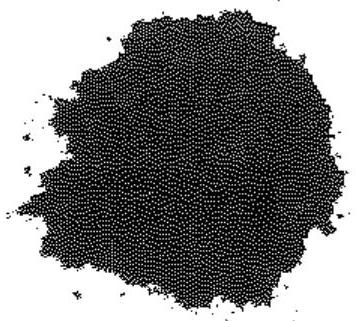
\includegraphics[max width=\textwidth, center]{2025_10_23_74efce88ce3a451fd6b0g-025(1)}

\begin{figure}[h]
\begin{center}
  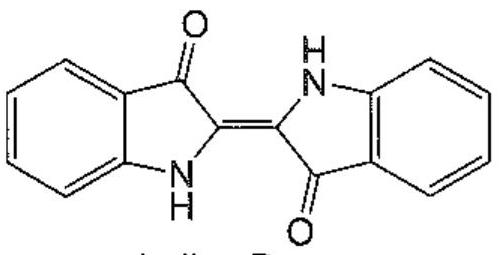
\includegraphics[width=\textwidth]{2025_10_23_74efce88ce3a451fd6b0g-025(2)}
\captionsetup{labelformat=empty}
\caption{Indigo Dye}
\end{center}
\end{figure}

\begin{center}
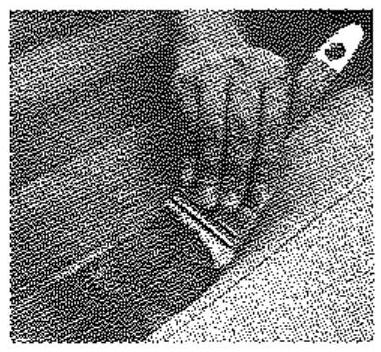
\includegraphics[max width=\textwidth]{2025_10_23_74efce88ce3a451fd6b0g-025}
\end{center}

\begin{figure}[h]
\begin{center}
  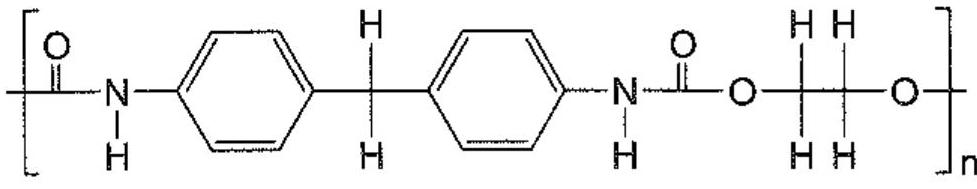
\includegraphics[width=\textwidth]{2025_10_23_74efce88ce3a451fd6b0g-025(3)}
\captionsetup{labelformat=empty}
\caption{Polyurethane}
\end{center}
\end{figure}

\begin{center}
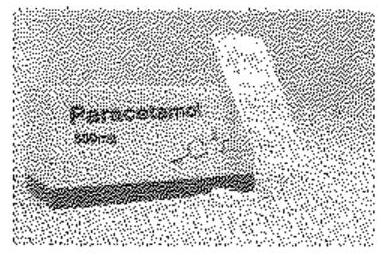
\includegraphics[max width=\textwidth]{2025_10_23_74efce88ce3a451fd6b0g-026}
\end{center}

$$
\overbrace{\mathrm{HO}} \overbrace{\mathrm{O}}^{\mathrm{H}}
$$

N -(4-hydroxyphenyl)acetamide\\
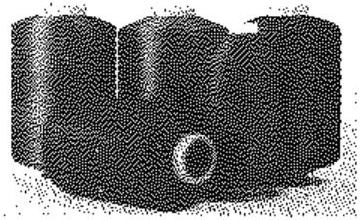
\includegraphics[max width=\textwidth, center]{2025_10_23_74efce88ce3a451fd6b0g-026(1)}\\
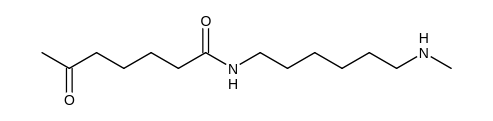
\includegraphics{smile-4905d81af2e8cc19d521fb8d7fb863597df45a06}

Nylon-6,6\\
8.23. Adrenaline là hormone dẫn truyền thần kinh chủ yếu được tiết ra bởi tuyến thượng thận. Nó đóng vai trò quan trọng trong phản ứng "chiến hoặc chạy" của cơ thể, nhanh chóng chuẩn bị cơ thể đối mặt với các tình huống căng thẳng hoặc nguy hiểm. Dopamine là chất dẫn truyền thần kinh có vai trò quan trọng trong việc điều khiển hệ thần kinh trung ương, đặc biệt ảnh hưởng đến việc tạo cảm giác hứng thú, động lực trong học tập, kiểm soát hành vi tư duy, trí nhở và ngồn ngữ,...\\
Cấu tạo của adrenaline và dopamine được mô tả dưới đây, hãy xác định các loại nhóm chức có trong mỗi chất và xác định bậc của nhóm chức (nếu có).\\
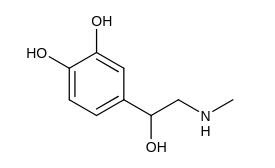
\includegraphics{smile-63685388f999004424d2de3d8986219fcaa90897}

adrenaline\\
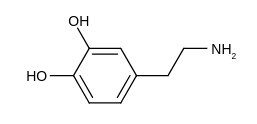
\includegraphics{smile-8dfc794d3352ef25dd8ba550722a5db4bc375b06}

dopamine\\
8.24. Dưới đây là hai phương pháp điều chế amine: (1) alkyl hoá ammonia và (2) khử hợp chất nitro. Hãy phân tích ưu và nhược điểm của mỗi phương pháp.\\
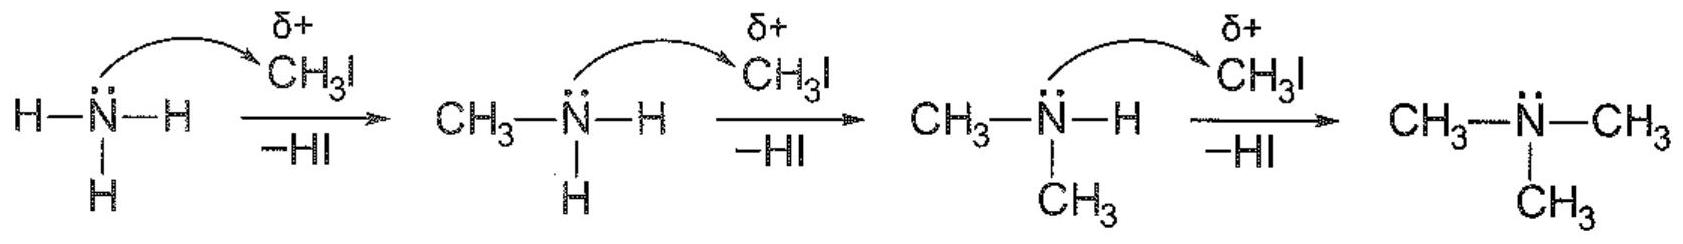
\includegraphics[max width=\textwidth, center]{2025_10_23_74efce88ce3a451fd6b0g-026(2)}

$$
\mathrm{C}_{6} \mathrm{H}_{5} \mathrm{NO}_{2}+6 \mathrm{H} \xrightarrow[t^{\circ}]{\mathrm{Fe}+\mathrm{HCl}} \mathrm{C}_{6} \mathrm{H}_{5} \mathrm{NH}_{2}+2 \mathrm{H}_{2} \mathrm{O}
$$

\section*{BÀI 9}
\section*{AMINO ACID VÀ PEPTIDE}
\section*{NHAN BIÉT}
9.1. Hợp chất nào sau đây là amino acid?\\
A. $\mathrm{H}_{2} \mathrm{NCH}_{2} \mathrm{COOCH}_{3}$.\\
B. $\mathrm{CH}_{3} \mathrm{NHCH}_{2} \mathrm{CH}_{3}$.\\
C. $\mathrm{H}_{2} \mathrm{NCH}_{2} \mathrm{COOH}$.\\
D. $\mathrm{HOCH}_{2} \mathrm{COOH}$.\\
9.2. Amino acid thiết yếu là các amino acid\\
A. có thể được tổng hợp bởi cơ thể con người.\\
B. phải được lấy thông qua chế độ ăn uống.\\
C. không cần thiết cho sức khoẻ con người.\\
D. chỉ được tìm thấy trong thực phẩm có nguồn gốc thực vật.\\
9.3. $\mathrm{H}_{2} \mathrm{~N}-\mathrm{CH}_{2}-\mathrm{COOH}$ tồn tại chính ở dạng\\
A. phân tữ trung hoà.\\
B. ion lưỡng cực.\\
C. cation.\\
D. anion.\\
9.4. Tính chất nào sau đây là tính chất vật lí đặc trưng của amino acid?\\
A. Nhiệt độ nóng chảy cao.\\
B. Không hoà tan trong nước.\\
C. Là chất khí ở nhiệt độ phòng.\\
D. Có độc tính rất cao.\\
9.5. Tính chất nào sau đây là tính chất hoá học đặc trưng của amino acid?\\
A. Tính oxi hoá mạnh.\\
B. Tính khử mạnh.\\
C. Tính lưỡng tính.\\
D. Tính acid mạnh.\\
9.6. Quá trình di chuyển của các amino acid trong điện trường được gọi là\\
A. sự điện dì.\\
B. sự điện li.\\
C. sự điện phân.\\
D. sự điện giải.\\
9.7. Loại liên kết được hình thành giữa các amino acid trong peptide được gọi là\\
A. liên kết ion.\\
B. liên kết hydrogen.\\
C. liên kết peptide.\\
D. liên kết cộng hoá trị.\\
9.8. Peptide là các hợp chất hữu cơ được tạo thành từ các\\
A. đơn vị glucose.\\
B. acid béo.\\
C. đơn vị $\alpha$-amino acid.\\
D. đơn vị hydrocarbon.\\
9.9. Chất nào dưới đây là một dipeptide?\\
A. Gly-Ala.\\
B. Gly-Ala-Val.\\
C. Gly-Gly-Ala-Val.\\
D. Val.\\
9.10. Phản ứng nào sau đây được sử dụng để nhận biết peptide?\\
A. Phản ứng màu với iodine.

B . Phản ứng màu biuret.\\
C. Phản ứng với thuốc thử Tollens.\\
D. Phản ứng với thuốc thử Fehling.

\section*{THONG HIEU}
Hãy chọn đúng hoặc sai cho mỗi ý a, $\mathrm{b}, \mathrm{c}, \mathrm{d}$ ở các câu 9.11-9.15.\\
9.11. Các phát biểu về cấu tạo của amino acid:\\
a) Chúng luôn chứa đồng thời nhóm amino và nhóm carboxyl.\\
b) Số nhóm carboxyl luôn nhiều hơn số nhóm amino.\\
c) Luôn tồn tại chủ yếu ở dạng ion lưỡng cực.\\
d) Trong Glu, số nhóm carboxyl nhiều hơn số nhóm amino.\\
9.12. Các phát biểu về tính chất của amino acid:\\
a) Đều là chất rắn ở điều kiện thường.\\
b) Thường tan tốt trong nước.\\
c) Vừa phản ứng được với acid mạnh, vừa phản ứng được với base mạnh.\\
d) Có thể phản ứng được với carboxylic acid tạo ester.\\
9.13. Một học sinh viết các phương trình hoá học minh hoạ tính chất hoá học của amino acid:\\
a) $\mathrm{H}_{2} \mathrm{NCH}_{2} \mathrm{COOH}+\mathrm{CH}_{3} \mathrm{CH}_{2} \mathrm{OH} \xrightarrow{\mathrm{H}_{2} \mathrm{SO}_{4}, \mathrm{t}^{\circ}} \mathrm{H}_{2} \mathrm{NCH}_{2} \mathrm{CH}_{2} \mathrm{COOCH}_{3}+\mathrm{H}_{2} \mathrm{O}$\\
b) $\mathrm{HCl}+\mathrm{H}_{2} \mathrm{NCH}\left(\mathrm{CH}_{3}\right) \mathrm{COOH} \longrightarrow \mathrm{ClH}_{3} \mathrm{NCH}\left(\mathrm{CH}_{3}\right) \mathrm{COOH}$\\
c) $\mathrm{H}_{2} \mathrm{NCH}\left(\mathrm{CH}_{3}\right) \mathrm{COOH}+\mathrm{NaOH} \longrightarrow \mathrm{H}_{2} \mathrm{NCH}\left(\mathrm{CH}_{3}\right) \mathrm{COONa}+\mathrm{H}_{2} \mathrm{O}$\\
d) $\mathrm{nH}_{2} \mathrm{~N}\left[\mathrm{CH}_{2}\right]_{5} \mathrm{COOH} \xrightarrow{\mathrm{xt}^{\mathrm{t}, \mathrm{t}^{\circ}}, \mathrm{p}}\left(\mathrm{HN}-\left[\mathrm{CH}_{2}\right]_{5}-\mathrm{CO}\right)_{\mathrm{n}}+\mathrm{nH}_{2} \mathrm{O}$\\
9.14. Các phát biểu về cấu tạo của peptide:\\
a) Peptide được cấu thành từ các đơn vị $\alpha$-và $\beta$-amino acid.\\
b) Tetrapeptide thường chứa bốn liên kết peptide trong phân tử.\\
c) Trong phân tử Gly-Ala-Val, thì Gly là amino acid đầu N.\\
d) Có thể điều chế bốn dipeptide khác nhau từ Gly và Val.\\
9.15. Các phát biểu về tính chất của peptide:\\
a) Thuỷ phân hoàn toàn Gly-Ala-Val thì thu được Gly, Ala và Val.\\
b) Thuỷ phân không hoàn toàn Gly-Ala-Val có thể thu được Gly-Ala và Ala-Val.\\
c) Gly-Ala-Val phản ứng với $\mathrm{Cu}(\mathrm{OH})_{2}$ trong môi trường kiềm tạo thành dung dịch màu tím.\\
d) Gly-Gly phản ứng hoàn toàn với dung dịch NaOH thu được $\mathrm{H}_{2} \mathrm{NCH}_{2} \mathrm{COONa}$.\\
9.16. Có bao nhiêu dipeptide khác nhau được hình thành từ alanine và glycine?\\
9.17. Tại sao các amino acid có nhiệt độ nóng chảy cao (đều là chất rắn ở điều kiện thường) và tan tốt trong nước?\\
9.18. Tại sao amino acid có tính lưỡng tính. Viết phương trình hoá học minh hoạ tính lưỡng tính của glycine.\\
9.19. Chỉ dùng quỳ tím, hãy phân biệt ba dung dịch sau: glycine, lysine và glutamic acid.

\section*{VAN DUNG}
9.20. Phân biệt amino acid tự nhiên, amino acid tiêu chuẩn và amino acid thiết yếu.\\
9.21. Viết dạng ion lưỡng cực cho các amino acid sau: glycine; alanine; valine; lysine và glutamic acid.\\
9.22. Thuỷ phân không hoàn toàn heptapeptide (F) thu được Ser-Asp-Phe (G), Ala-His-Ser $(\mathrm{H})$ và Phe-Ala $(\mathrm{I})$. Biết Ala là amino acid đầu C trong F. Hãy cho biết trật tự liên kết giữa các amino acid trong F .\\
9.23. Enkephalin $(\mathrm{A})$ là các cấu tử pentapeptide của các endorphin. Xác định trật tự các amino acid trong A từ các dữ kiện sau: Thuỷ phân hoàn toàn A thu được Gly, Phe, Leu và Tyr; thuỷ phân không hoàn toàn A thu được Gly-Gly-Phe và Tyr-Gly. Biết Tyr (tyrosine) là amino acid đầu N.\\
9.24. Thuỷ phân hoàn toàn Bradykinin (B) thu được: 2Arg, Gly, 2Phe, 3Pro và Ser. Thuỷ phân không hoàn toàn B thu được Pro-Pro-Gly, Ser-Pro-Phe, Pro-GlyPhe, Arg-Pro và Phe-Ser. Biết Arg là amino acid đầu C. Xác định trật tự liên kết của các amino acid trong B .

\section*{BÀI 10 \\
 PROTEIN VÀ ENZYME}
\section*{NHAN BIET}
10.1. Mỗi chuỗi polypeptide gồm các đơn vị ...(1)... liên kết với nhau qua ...(2)... theo một trật tự nhất định. Các cụm từ phù hợp cho mỗi khoảng trống trong câu trên lần lượt là\\
A. $\alpha$-amino acid và liên kết peptide.\\
B. monosaccharide và liên kết glycoside.\\
C. $\alpha$-amino acid và liên kết glycoside.\\
D. monosaccharide và liên kết peptide.\\
10.2. Loại hợp chất nào sau đây chứa các thành phần "phi protein" như nucleic acid, lipid, carbohydrate?\\
A. Protein đơn giản.\\
B. Protein phức tạp.\\
C. Chất béo.\\
D. Polysaccharide.\\
10.3. Protein không tham gia loại phản ứng nào dưới đây?\\
A. Phản ứng thuỷ phân.\\
B. Phản ứng màu với $\mathrm{Cu}(\mathrm{OH})_{2}$.\\
C . Phản ứng màu với $\mathrm{HNO}_{3}$.\\
D. Phản ứng khử thành alcohol.

Hãy chọn đúng hoặc sai cho mỗi ý $\mathrm{a}, \mathrm{b}, \mathrm{c}, \mathrm{d}$ ở các câu $10.4-10.5$.\\
10.4. Các phát biểu về protein:\\
a) Protein phản ứng với nitric acid tạo chất rắn màu đỏ.\\
b) Protein phản ứng với copper(II) hydroxide tạo sản phẩm màu tím.\\
c) Phản ứng đông tụ của protein có thể xảy ra dưới tác động của nhiệt độ.\\
d) Quá trình thuỷ phân hoàn toàn protein đơn giản tạo thành các $\alpha$-amino acid.\\
10.5. Các phát biểu về enzyme:\\
a) Phần lớn enzyme là những protein xúc tác cho các phản ứng hoá học và sinh hoá.\\
b) Mỗi enzyme chỉ xúc tác cho một hoặc một số phản ứng nhất định.\\
c) Enzyme có hoạt tính xúc tác cao hơn xúc tác hoá học của cùng quá trình.\\
d) Enzyme có nhiều ứng dụng trong công nghệ sinh học.

\section*{THONG HIEU}
10.6. Cho các protein sau: keratin (có ở tóc, móng); collagen (có ở da, sụn); myosin (có ở cơ bắp); hemoglobin (có ở máu) và albumin (có ở lòng trắng trứng). Có bao nhiêu protein có thể tan được trong nước tạo dung dịch keo?\\
10.7. Cho các điều kiện sau: (1) môi trường acid; (2) môi trường base; (3) đun nóng và (4) sự có mặt của ion kim loại nặng. Có bao nhiêu điều kiện gây ra sự đông tụ của protein?\\
10.8. Cho các vai trò với sự sống của chất như. (1) tham gia xây dựng tế bào; (2) vận chuyển các chất trong cơ thể; (3) điều hoà quá trình trao đổi chất; (4) xúc tác cho các phản ứng hoá sinh; (5) giúp cơ thể chống lại tác nhân có hại. Protein có thể đảm nhận bao nhiêu vai trò?\\
10.9. Nêu vai trò chính của các enzyme amylase (tạo ra ở nước bọt và tuyến tuỵ) và maltase (tạo ra ở niêm mạc ruột non) trong cơ thể người.\\
10.10. Tại sao một số người không thể tiêu hoá sữa?

\section*{VAN DUNG}
10.11. Tại sao cần có sự đa dạng thịt, cá, trứng, sữa trong khẩu phần ăn?\\
10.12. Viết phương trình hoá học của bốn phản ứng có xúc tác enzyme mà em đã học.

\section*{BÀI 11}
\section*{ÔN TÂP CHƯONG III}
\section*{NHAN BIÉT}
11.1. Nhóm chức nào sau đây là đặc trưng cho amine?\\
A. -OH .\\
B. -COOH .\\
C. $-\mathrm{NH}_{2}$.\\
D. -CHO .\\
11.2. Chất nào sau đây là aryl amine?\\
A. $\mathrm{C}_{6} \mathrm{H}_{5}-\mathrm{NH}_{2}$.\\
B. $\mathrm{C}_{2} \mathrm{H}_{5}-\mathrm{NH}_{2}$.\\
C. $\mathrm{C}_{6} \mathrm{H}_{5}-\mathrm{CH}_{2}-\mathrm{CH}_{2}-\mathrm{CH}_{3}$.\\
D. $\left(\mathrm{CH}_{3}\right)_{3} \mathrm{~N}$.\\
11.3. Methyl amine không phản ứng với chất nào nào sau đây?\\
A. Dung dịch NaOH .\\
B. Dung dịch HCl .\\
C. Dung dịch $\mathrm{CuSO}_{4}$.\\
D. $\mathrm{HNO}_{2}$ trong HCl .\\
11.4. Amino acid chứa nhóm chức nào sau đây?\\
A. Chỉ có nhóm amine.\\
B. Chỉ có nhóm carboxyl.\\
C. Cả nhóm amine và nhóm carboxyl.\\
D. Cả nhóm amine và nhóm hydroxyl.\\
11.5. Dạng tồn tại chính của amino acid là dạng nào sau đây?\\
A. Phân tử trung hoà.\\
B. Ion lưỡng cực.\\
C. Cation.\\
D. Anion.\\
11.6. Phản ứng nào sau đây không phải là tính chất hoá học của amino acid?\\
A. Phản ứng với acid.\\
B. Phản ứng với kiềm.\\
C. Phản ứng tạo ether.\\
D. Phản ứng trùng ngưng.\\
11.7. Nhóm peptide có cấu tạo là\\
A. $-\mathrm{CO}-\mathrm{O}-$.\\
B. $-\mathrm{CO}-\mathrm{NH}-$.\\
C. $-\mathrm{CO}-\mathrm{NH}_{2}$.\\
D. $-\mathrm{CO}-$.\\
11.8. Trong cơ thể, enzyme có chức năng nào sau đây?\\
A. Cấu trúc tế bào.\\
B. Chất điện giải.\\
C. Chất dự trữ năng lượng.\\
D. Xúc tác sinh học.\\
11.9. Phản ứng của amine với $\mathrm{Cu}(\mathrm{OH})_{2}$ tạo sản phẩm có màu\\
A. vàng nhạt.\\
B. đỏ nâu.\\
C. xanh lam.\\
D. không màu.

\section*{THONG HILU}
11.10. Tại sao amino acid có thể tồn tại ở dạng ion lưỡng cực trong môi trường nước?\\
A. Do có tính chất anion của nhóm carboxyl.\\
B. Do có khả năng hình thành liên kết hydrogen.\\
C. Do khả năng chuyển dịch proton giữa nhóm amine và nhóm carboxyl.\\
D. Do tính chất lưỡng tính của nhóm amine.\\
11.11. Nhóm $-\mathrm{NH}_{2}$ của amine thể hiện tính chất hoá học nào sau đây?\\
A. Tính acid do có thể nhận proton.\\
B. Tính base do có thể nhận proton.\\
C. Tính oxi hoá do có thể nhường electron.\\
D. Tính khử do có thể nhường proton.\\
11.12. Trong phản ứng với nước bromine, aniline thể hiện phản ứng nào sau đây?\\
A. Phản ứng cộng halogen vào nhóm $-\mathrm{NH}_{2}$.\\
B. Phản ứng thế hydrogen của nhóm $-\mathrm{NH}_{2}$.\\
C. Phản ứng cộng hợp halogen vào vòng benzene.\\
D. Phản ứng thế hydrogen trên vòng benzene.\\
11.13. Nhận định nào sau đây không đúng khi so sánh peptide với protein?\\
A. Peptide thường có khối lượng mol phân tử thấp hơn protein.\\
B. Protein thường chứa nhiều chuỗi polypeptide.\\
C. Peptide không có cấu trúc phân tử phức tạp như protein.\\
D. Peptide và protein đều không thể thực hiện các chức năng sinh học.\\
11.14. Trong phản ứng của amine với $\mathrm{Cu}(\mathrm{OH})_{2}$, sản phẩm có màu xanh đặc trưng là do\\
A. sự hình thành phức giữa ion $\mathrm{Cu}^{2+}$ và nhóm $-\mathrm{NH}_{2}$.\\
B. sự oxi hoá của ion $\mathrm{Cu}^{2+}$ khi tiếp xúc với amine.\\
C. phản ứng giữa ion hydroxide và nhóm $-\mathrm{NH}_{2}$.\\
D. sự giải phóng khí hydrogen khi amine phản ứng với ion $\mathrm{Cu}^{2+}$.\\
11.15. Trong phản ứng màu biuret, peptide và protein tạo ra sản phẩm màu tím là do\\
A. sự kết tủa của ion đồng.\\
B. sự tạo thành liên kết hydrogen.\\
C. sự hình thành phức chất giữa ion đồng và nhóm peptide liên kết.\\
D. sự phản ứng của ion đồng với nhóm $-\mathrm{NH}_{2}$.

\section*{Hãy chọn đúng hoăc sai cho mỗi ý a, $b, c, d$ ở các câu 11.16-11.18.}
11.16. a) Tất cả amine đều là dẫn xuất của ammonia.\\
b) Phản ứng của amine với HCl tạo ra muối ammonium chloride.\\
c) Peptide là chuỗi liên kết của nhiều amino acid thông qua liên kết peptide.\\
d) Tất cả enzyme đều là protein.\\
11.17. a) Amino acid không thể phản ứng với carboxylic acid.\\
b) Tất cả amine đều phản ứng được với $\mathrm{Cu}(\mathrm{OH})_{2}$ để tạo phức màu xanh.\\
c) Tất cả các amino acid thiên nhiên đều có ít nhất một nhóm amino và một nhóm carboxyl.\\
d) Protein tham gia vào tất cả các quá trình sinh hoá diễn ra trong cơ thể.\\
11.18. a) Protein không thể đóng vai trò như một xúc tác troñg các phản ứng hoá học.\\
b) Peptide và protein có cùng cấu tạo hoá học cơ bản.\\
c) Tất cả peptide đều có khả năng tạo phức màu tím trong phản ứng màu biuret.\\
d) Mỗi enzyme chỉ xúc tác cho một phản ứng hoặc một số phản ứng nhất định.

\section*{VAN DUNG}
11.19. Hãy viết phương trình hoá học của phản ứng chuyển hoá từ benzene $\left(\mathrm{C}_{6} \mathrm{H}_{6}\right)$ thành nitrobenzene $\left(\mathrm{C}_{6} \mathrm{H}_{5} \mathrm{NO}_{2}\right)$.\\
11.20. Tại sao dung dịch aniline gần như không làm đổi màu quỳ tím?\\
11.21. Cho các dung dịch sau: (1) glycine; (2) lysine và (3) glutamic acid. Các dung dịch trên làm đổi màu quỳ tím như thế nào? Giải thích.

\section*{Chuong IV POLYMER}
\section*{BÀI 12 \\
 ĐAI CUÓNG VỀ POLYMER}
\section*{NHAN BIÉT}
12.1. Chất nào dưới đây thuộc loại polymer?\\
A. Glucose.\\
B. Fructose.\\
C. Saccharose.\\
D. Cellulose.\\
12.2. Tính chất vật lí chung của polymer là\\
A. chất lỏng, không màu, không tan trong nước.\\
B. chất lỏng, không màu, tan tốt trong nước.\\
C. chất rắn, không bay hơi, dễ tan trong nước.\\
D. chất rắn, không bay hơi, không tan trong nước.\\
12.3. Polyethylene là sản phẩm của phản ứng trùng hợp của chất nào dưới đây?\\
A. $\mathrm{CH}_{2}=\mathrm{CH}-\mathrm{Cl}$.\\
B. $\mathrm{CH}_{2}=\mathrm{CH}_{2}$.\\
C. $\mathrm{CH}_{2}=\mathrm{CH}-\mathrm{C}_{6} \mathrm{H}_{5}$.\\
D. $\mathrm{CH}_{2}=\mathrm{CH}-\mathrm{CH}_{3}$.\\
12.4. Chất có thể trùng hợp tạo ra polymer là\\
A. $\mathrm{C}_{2} \mathrm{H}_{5} \mathrm{OH}$.\\
B. $\mathrm{CH}_{3} \mathrm{COOH}$.\\
C. $\mathrm{CH}_{3} \mathrm{CH}_{3}$.\\
D. $\mathrm{CH}_{2}=\mathrm{CHCH}_{3}$.\\
12.5. Polymer nào dưới đây có chứa nguyên tố chlorine?\\
A. PE.\\
B. PP.\\
C. PVC.\\
D. PS.\\
12.6. Polymer nào sau đây thuộc loại polymer tổng hợp?\\
A. Tinh bột.\\
B. Tơ tằm.\\
C. Polyethylene.\\
D. Cao su thiên nhiên.\\
12.7. Quá trình lưu hoá cao su thuộc loại phản ứng\\
A. cắt mạch polymer.\\
B. tăng mạch polymer.\\
C. giữ nguyên mạch polymer.\\
D. phân huỷ polymer.

\section*{THONG HIEU}
12.8. Chất nào dưới đây không phải là polymer?\\
A. Lipid.\\
B. Tinh bột.\\
C. Cellulose.\\
D. Protein.\\
12.9. Poly(methyl methacrylate) (PMMA) cho ánh sáng truyền qua trên $90 \%$ nên được sử dụng làm thuỷ tinh hữu cơ. Thực hiện phản ứng trùng hợp monomer nào sau đây thu được PMMA?\\
A. $\mathrm{CH}_{2}=\mathrm{C}\left(\mathrm{CH}_{3}\right) \mathrm{COOCH}_{3}$.\\
B. $\mathrm{CH}_{2}=\mathrm{CHCOOCH}_{3}$.\\
C. $\mathrm{CH}_{2}=\mathrm{CHC}_{6} \mathrm{H}_{5}$.\\
D. $\mathrm{CH}_{2}=\mathrm{CHCl}$.\\
12.10. Polymer nào sau đây trong thành phần hoá học chỉ có hai nguyên tố carbon và hydrogen?\\
A. Poly(methyl methacrylate).\\
B. Poly(vinyl chloride).\\
C. Poly(phenol formaldehyde).\\
D. Polystyrene.

\section*{Hãy chọn đúng hoặc sai cho mỗi ý $a, b, c, d$ ở câu sau.}
12.11. a) Monomer là các phân tử nhỏ có khả năng kết hợp với nhau tạo nên polymer.\\
b) Polymer là những chất có khối lượng phân tử nhỏ.\\
c) Hầu hết polymer là những chất rắn, không bay hơi và không tan trong nước.\\
d) Polymer là những chất có khối lượng phân tử rất lớn do nhiều mắt xích liên kết với nhau tạo nên.\\
12.12. Một mẫu polystyrene ( PS ) được dùng làm hộp xốp bảo quản thực phẩm có chứa hỗn hợp gồm nhiều đoạn mạch PS có số mắt xích khác nhau và có phân tử khối trung bình là 264160 . Tính số mắt xích trung bình của mẫu PS đó.

\section*{VAN DUNG}
12.13. Các động vật ăn cỏ như trâu, bò, dê, cừu,... có thể chuyển hoá cellulose trong thức ăn thành glucose bằng enzyme cellulase để cung cấp năng lượng cho cơ thể. Phản ứng chuyển hoá cellulose thành glucose thuộc loại phản ứng nào sau đây?\\
A. Cắt mạch polymer.\\
B. Giữ nguyên mạch polymer.\\
C. Tăng mạch polymer.\\
D. Trùng ngưng.

Hãy chọn đúng hoăc sai cho mỗi ý $a, b, c, d$ ở câu sau.\\
12.14. Polymer X có thể chịu được nhiệt độ lên tới $160^{\circ} \mathrm{C}$ nên được dùng làm ống dẫn nước nóng, hộp đựng thực phẩm có thể sữ dụng trong lò vi sóng,... Các vật dụng làm từ $X$ thường được in kí hiệu như hình bên.\\
a) X được tổng hợp từ phản ứng trùng hợp pent-1-ene.\\
b) Hộp nhựa làm từ X có thể đựng nước sôi mà không bị biến dạng.\\
c) $X$ thuộc loại polymer nhiệt dẻo.\\
d) Nhựa làm từ $X$ thuộc loại nhựa có thể tái chế.\\
12.15. Sợi Kevlar có độ bền lớn nên được sử dụng làm sợi gia cường trong lốp xe đua, vật liệu composite, vải thuyền buồm, áo giáp chống đạn,... Kevlar có công thức cấu tạo như hình sau đây.\\
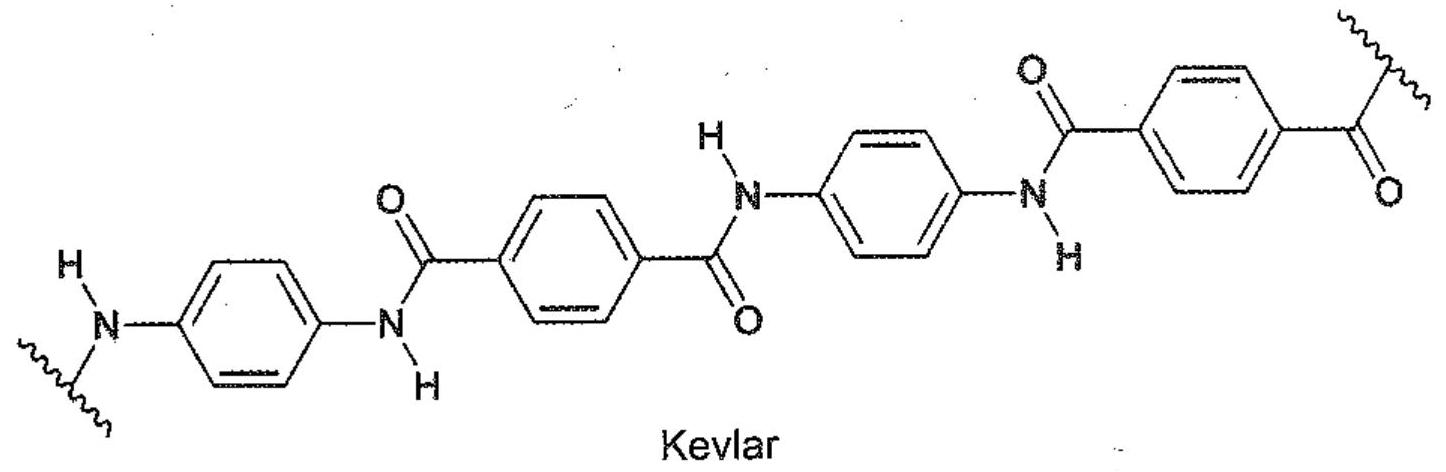
\includegraphics[max width=\textwidth, center]{2025_10_23_74efce88ce3a451fd6b0g-037}

Viết phương trình hoá học tổng hợp Kevlar từ các monomer tương ứng. Phản ứng đó thuộc loại phản ứng trùng hợp hay trùng ngưng?\\
12.16. Poly(vinyl alcohol) (viết tắt là PVA) được dùng làm chất kết dính, sợi vinylon, vật liệu ứng dụng trong y tế,... Polyvinyl acetate (viết tắt là PVAc) được sử dụng phổ biến làm keo dán gỗ, keo dán giấy,... PVAc và PVA được tổng hợp theo sơ đồ sau đây:

$$
\mathrm{HC} \equiv \mathrm{CH} \xrightarrow{+\mathrm{CH}_{3} \mathrm{COOH}} \mathrm{~A} \xrightarrow{\text { trùng hợp }} \mathrm{PVAc} \xrightarrow{\mathrm{NaOH}, \mathrm{t}^{\circ}} \mathrm{PVA}
$$

a) Viết phương trình hoá học hoàn thành sơ đồ chuyển hoá trên.\\
b) PVA là một polymer có khả năng hoà tan được trong nước. Giải thích.

\section*{BÀI 13}
\section*{VÂT LIỆU POLYMER}
\section*{NHAN BIET}
13.1. Polypropylene là chất dẻo được sử dụng phổ biến thử hai sau polyethylene. Trùng hợp chất nào sau đây thu được polypropylene?\\
A. $\mathrm{CH}_{2}=\mathrm{CH}-\mathrm{Cl}$.\\
B. $\mathrm{CH}_{2}=\mathrm{CH}_{2}$.\\
C. $\mathrm{CH}_{2}=\mathrm{CH}-\mathrm{C}_{6} \mathrm{H}_{5}$.\\
D. $\mathrm{CH}_{2}=\mathrm{CH}-\mathrm{CH}_{3}$.\\
13.2. Trùng hợp monomer $\mathrm{CH}_{2}=\mathrm{CH}-\mathrm{Cl}$ thu được chất dẻo nào sau đây?\\
A. PE.\\
B. PP.\\
C. PVC.\\
D. PS.\\
13.3. Tơ sợi nào sau đây thuộc loại tơ tự nhiên?\\
A. Sợi bông.\\
B. Nitron.\\
C. Nylon-6,6.\\
D. Cellulose acetate.\\
13.4. Cao su lưu hoá thu được khi cho cao su tác dụng với chất nào sau đây?\\
A. Lưu huỳnh.\\
B. $\mathrm{Na}_{2} \mathrm{SO}_{3}$.\\
C. $\mathrm{Na}_{2} \mathrm{SO}_{4}$.\\
D. Styrene.\\
13.5. Trùng hợp chất nào sau đây thu được polyacrylonitrile dùng để sản xuất tơ nitron?\\
A. $\mathrm{CH}_{2}=\mathrm{CH}-\mathrm{Cl}$.\\
B. $\mathrm{CH}_{2}=\mathrm{CH}-\mathrm{CN}$.\\
C. $\mathrm{CH}_{2}=\mathrm{CH}_{2}$.\\
D. $\mathrm{CH}_{2}=\mathrm{CH}-\mathrm{CH}_{3}$.\\
13.6. Trùng hợp chất nào sau đây thu được cao su buna?\\
A. $\mathrm{CH}_{2}=\mathrm{CH}-\mathrm{CH}=\mathrm{CH}_{2}$.\\
B. $\mathrm{CH}_{2}=\mathrm{CCl}-\mathrm{CH}=\mathrm{CH}_{2}$.\\
C. $\mathrm{CH}_{2}=\mathrm{C}\left(\mathrm{CH}_{3}\right)-\mathrm{CH}=\mathrm{CH}_{2}$.\\
D. $\mathrm{CH}_{2}=\mathrm{C}\left(\mathrm{CH}_{3}\right)-\mathrm{CCl}=\mathrm{CH}_{2}$.\\
13.7. Cho các chất sau:\\
$\mathrm{CH}_{2}=\mathrm{CHCl} ; \mathrm{CH}_{2}=\mathrm{CHCH}_{3} ; \mathrm{CH}_{2}=\mathrm{CH}-\mathrm{CH}=\mathrm{CH}_{2} ; \mathrm{H}_{2} \mathrm{~N}\left[\mathrm{CH}_{2}\right]_{5} \mathrm{COOH}$.\\
Số chất có khả năng tham gia phản ứng trùng hợp là\\
A. 3 .\\
B. 1 .\\
C. 4 .\\
D. 2 .

\section*{THONG HIEU}
13.8. Trên hộp xốp cách nhiệt, hộp đựng thức ăn mang về, cốc, chén đĩa dùng một lần,... thường được in kí kiệu như hình bên. Polymer dùng làm các đồ dùng đó được tổng hợp từ monomer nào sau đây?\\
A. $\mathrm{CH}_{2}=\mathrm{CH}_{2}$.\\
B. $\mathrm{CH}_{2}=\mathrm{CHCH}_{3}$.\\
C. $\mathrm{CH}_{2}=\mathrm{CHC}_{6} \mathrm{H}_{5}$.\\
D. $\mathrm{CH}_{2}=\mathrm{CHCl}$.\\
13.9. Phân tử polymer nào sau đây chỉ chứra hai loại nguyên tố?\\
A. Poly(methyl methacrylat).\\
B. Poly(vinyl chloride).\\
C. Polyacrylonitrile.\\
D. Polypropylene.\\
13.10. Polymer nào sau đây không thuộc loại chất dẻo?\\
A. Poly(methyl methacrylate).\\
B. Poly(vinyl chloride).\\
C. Polystyrene.\\
D. Polbuta-1,3-diene.\\
13.11. Cao su buna-S (hay còn gọi là cao su SBR ) là loại cao su tổng hợp được sử dụng rất phổ biến, ước tính $50 \%$ lốp xe được làm từ SBR . Thực hiện phản ứng trùng hợp các chất nào dưới đây thu được sản phẩm là cao su buna-S?\\
A. $\mathrm{CH}_{2}=\mathrm{CHCH}=\mathrm{CH}_{2}$ và $\mathrm{C}_{6} \mathrm{H}_{5} \mathrm{CH}=\mathrm{CH}_{2}$.\\
B. $\mathrm{CH}_{2}=\mathrm{CHCH}=\mathrm{CH}_{2}$ và sulfur.\\
C. $\mathrm{CH}_{2}=\mathrm{CHCH}=\mathrm{CH}_{2}$ và $\mathrm{CH}_{2}=\mathrm{CHCl}$.\\
D. $\mathrm{CH}_{2}=\mathrm{CHCH}=\mathrm{CH}_{2}$ và $\mathrm{CH}_{2}=\mathrm{CHCN}$.

\section*{Hãy chọn đúng hoăc sai cho mỗi ý $a, b, c, d$ ở câu sau.}
13.12. a) Chất dẻo dễ bị biến dạng ở nhiệt độ cao.\\
b) Tơ polyamide thuộc loại tơ bán tổng hợp.\\
c) Cao su là những vật liệu polymer bị biến dạng dưới tác dụng của lực bên ngoài và vẫn giữ nguyên biến dạng đó khi thôi tác dụng.\\
d) Vật liệu composite thường gồm hai thành phần chính là vật liệu cốt và vật liệu nền.\\
13.13. Gỗ nhựa hiện nay được dùng phổ biến để thay thế gỗ tự nhiên do có một số tính chất ưu việt. Một loại gỗ nhựa được làm từ bột gỗ và nhựa polyethylene tái chế. Xác định vật liệu cốt và vật liệu nền trong loại gỗ nhựa đó.

\section*{VAN DUNG}
13.14. Cao su butyl có khả năng chống thấm khí tốt, chống chịu hoá chất nên được sử dụng làm lớp lót trong săm lốp, găng tay cao su,... Cao su butyl thường được sản xuất bằng cách trùng hợp $98 \%$ monomer X với $2 \%$ monomer Y . Dưới đây là một đoạn mạch của cao su butyl:\\
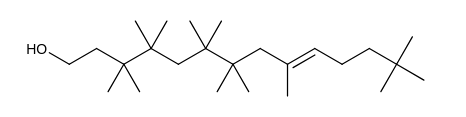
\includegraphics{smile-82c26c7cec4af5176c97cca85493f39f4cb3f80d}

X và Y lần lượt là các chất nào sau đây?\\
A. $\mathrm{C}\left(\mathrm{CH}_{3}\right)_{2}=\mathrm{CH}-\mathrm{CH}=\mathrm{CH}_{2}$ và $\mathrm{CH}_{2}=\mathrm{CH}\left(\mathrm{CH}_{3}\right)$.\\
B. $\mathrm{CH}_{2}=\mathrm{C}\left(\mathrm{CH}_{3}\right)_{2}$ và $\mathrm{CH}_{2}=\mathrm{C}\left(\mathrm{CH}_{3}\right)-\mathrm{CH}=\mathrm{CH}_{2}$.\\
C. $\mathrm{CH}_{2}=\mathrm{C}\left(\mathrm{CH}_{3}\right)-\mathrm{CH}=\mathrm{CH}_{2}$ và $\mathrm{CH}_{2}=\mathrm{C}\left(\mathrm{CH}_{3}\right)_{2}$.\\
D. $\mathrm{CH}_{2}=\mathrm{C}\left(\mathrm{CH}_{3}\right)_{2}$ và $\mathrm{C}\left(\mathrm{CH}_{3}\right)_{2}=\mathrm{CH}-\mathrm{CH}=\mathrm{CH}_{2}$.

Hãy chọn đúng hoăc sai cho mỗi ý a, $b, c, d$ ở các câu 13.15-13.16.\\
13.15. a) Các polymer nhiệt dẻo đều có thể tái chế do chúng bị nóng chảy ở nhiệt độ cao.\\
b) Các polymer có mạch không phân nhánh đều có thể dùng làm tơ.\\
c) Cao su lưu hoá có cấu trúc mạng lưới không gian.\\
d) Vật liệu nền đảm bảo cho composite có được các đặc tính cơ học cần thiết.\\
13.16. Poly(butylene adipate terephthalate) (PBAT) là một polymer có khả năng phân huỷ sinh học, có tên thương mại là Ecoflex. PBAT có đặc tính tương tự như polyethylene mật độ thấp (LDPE) nên nó được sử dụng làm túi nylon, bao bì thực phẩm phân huỷ sinh học. PBAT được điều chế từ ba monomer sau đây:\\
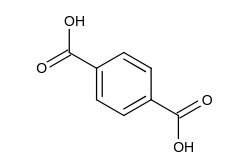
\includegraphics{smile-91c82a8bf17aed5d23c7af2c1161766fb5014fec}

$$
\mathrm{HO}-\left[\mathrm{CH}_{2}\right]_{4}-\mathrm{OH} \text { và } \mathrm{HOOC}-\left[\mathrm{CH}_{2}\right]_{4}-\mathrm{COOH}
$$

a) PBAT thuộc loại polyester.\\
b) Phản ứng tổng hợp PBAT thuộc loại phản ứng trùng hợp.\\
c) Một mắt xích PBAT gồm 3 nhóm ester.\\
d) Túi nylon làm từ PBAT thân thiện môi trường hơn so với LDPE .\\
13.17. Polymer A thuộc loại poly(ester amide) được sử dụng trong dược phẩm để giải phóng thuốc có kiểm soát. Sau khi uống, các enzyme của cơ thể nhận biết các amino acid tự nhiên trong mạch polymer và phân cắt tại các vị trí này làm thuốc được giải phóng một cách từ từ. A được tổng hợp từ bốn monomer gồm hai monomer đa chức, hai monomer là amino acid và dẫn xuất của amino acid. A có công thức cấu tạo như hình sau đây.\\
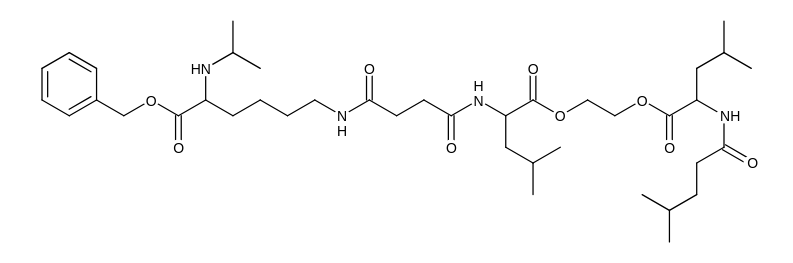
\includegraphics{smile-7f6755c6e1c2022dd8df503bac03fd1ac082ea73}

Xác định công thức cấu tạo của bốn monomer cấu thành nên A .

\section*{BÀI 14}
\section*{ÔN TÂP CHƯONG IV}
\section*{NHAN BIET}
14.1. Poly(vinyl chloride) (PVC) là một loại chất dẻo phổ biến, được sử đụng làm vỏ dây điện, ống dẫn nước thải, áo mưa, vải giả da,... PVC có công thức cấu tạo là:\\
A. $\left(-\mathrm{CH}_{2}-\mathrm{CH}_{2}\right) \frac{}{n}$\\
B. $\left(-\mathrm{CH}_{2}-\underset{\mathrm{CH}_{3}}{\mathrm{CH}}\right)_{n}$\\
C. $\left(\mathrm{CH}_{2}-\underset{\mathrm{C}_{6} \mathrm{H}_{5}}{\mathrm{CH}}\right)^{n}$\\
D. $\left(-\mathrm{CH}_{2}-\underset{\mathrm{Cl}}{\mathrm{CH}}\right)_{n}$\\
14.2. Tơ tằm, sợi bông, len thuộc loại tơ nào sau đây?\\
A. Tơ tự nhiên.\\
B. Tơ tổng hợp.\\
C. Tơ bán tổng hợp.\\
D. Tơ nhân tạo.\\
14.3. Tính chất đặc trưng của cao su là\\
A. tính đàn hồi.\\
B. tính dẻo.\\
C. dễ kéo thành sợi mảnh.\\
D. dễ tan trong nước.\\
14.4. Trùng hợp chất nào sau đây thu được cao su isoprene?\\
A. $\mathrm{CH}_{2}=\mathrm{CH}-\mathrm{CH}=\mathrm{CH}_{2}$.\\
B. $\mathrm{CH}_{2}=\mathrm{CCl}-\mathrm{CH}=\mathrm{CH}_{2}$.\\
C. $\mathrm{CH}_{2}=\mathrm{C}\left(\mathrm{CH}_{3}\right)-\mathrm{CH}=\mathrm{CH}_{2}$.\\
D. $\mathrm{CH}_{2}=\mathrm{C}\left(\mathrm{CH}_{3}\right)-\mathrm{C}\left(\mathrm{CH}_{3}\right)=\mathrm{CH}_{2}$.\\
14.5. Chất nào sau đây có thể tham gia phản ứng trùng ngưng?\\
A. $\mathrm{CH}_{2}=\mathrm{CH}_{2}$.\\
B. $\mathrm{CH}_{2}=\mathrm{CHCH}_{3}$.\\
C. $\mathrm{CH}_{2}=\mathrm{CHC}_{6} \mathrm{H}_{5}$.\\
D. $\mathrm{H}_{2} \mathrm{~N}\left[\mathrm{CH}_{2}\right]_{5} \mathrm{COOH}$.

\section*{THONG HISU}
14.6. Polymer nào sau đây không thuộc loại cao su?\\
A. Poly(methyl methacrylate).\\
B. Polychloroprene.\\
C. Polyisoprene.\\
D. Polybuta-1,3-diene.\\
14.7. Tơ nào sau đây thuộc loại tơ bán tổng hợp ?\\
A. Tơ nylon-6,6.\\
B. To cellulose acetate.\\
C. Tơ capron.\\
D. Tơ tằm.\\
14.8. LDPE là một chất dẻo dễ tạo màng, có tính dai bền nên được sử dụng làm túi nỷlon, màng bọc, bao gói thực phẩm. Trên các bao bì làm từ LDPE thường được in kí kiệu như hình bên. LDPE được tổng hợp từ monomer nào sau đây?\\
A. $\mathrm{CH}_{2}=\mathrm{CH}_{2}$.\\
B. $\mathrm{CH}_{2}=\mathrm{CHCH}_{3}$.\\
C. $\mathrm{CH}_{2}=\mathrm{CHC}_{6} \mathrm{H}_{5}$.\\
D. $\mathrm{CH}_{2}=\mathrm{CHCl}$.\\
14.9. Cao su buna-N (hay còn gọi là cao su nitrile, có kí hiệu là NBR) là loại cao su tổng hợp có khả năng chịu dầu mỡ tốt nên được dùng làm ống dẫn nhiên liệu, gioăng phớt làm kín trong các máy móc. Thực hiện phản ứng trùng hợp các chất nào dưới đây thu được sản phẩm là cao su buna-N?\\
A. $\mathrm{CH}_{2}=\mathrm{CHCH}=\mathrm{CH}_{2}$ và $\mathrm{C}_{6} \mathrm{H}_{5} \mathrm{CH}=\mathrm{CH}_{2}$.\\
B. $\mathrm{CH}_{2}=\mathrm{C}\left(\mathrm{CH}_{3}\right) \mathrm{CH}=\mathrm{CH}_{2}$ và $\mathrm{CH}_{2}=\mathrm{CHCN}$.\\
C. $\mathrm{CH}_{2}=\mathrm{CHCH}=\mathrm{CH}_{2}$ và $\mathrm{N}_{2}$.\\
D. $\mathrm{CH}_{2}=\mathrm{CHCH}=\mathrm{CH}_{2}$ và $\mathrm{CH}_{2}=\mathrm{CHCN}$.

\section*{Hãy chọn đúng hoặc sai cho mỗi ý a, b, c, d ở câu sau.}
14.10. a) Polypropylene là một polymer có cấu trúc mạch phân nhánh.\\
b) Cao su sau khi lưu hoá có các tính chất lí, hoá nổi trội hơn cao su ban đầu.\\
c) Tơ nylon- 6,6 kém bền trong môi trường kiềm mạnh.\\
d) Nhựa polymer thường được làm vật liệu nền trong composite.

\section*{VAN DUNG}
Hãy chọn đúng hoặc sai cho mỗi ý $a, b, c, d$ ở câu sau.\\
14.11. a) Các polymer nhiệt rắn bị nóng chảy khi đun nóng.\\
b) Mạch polymer trong tơ thường có cấu tạo không phân nhánh.\\
c) Cao su buna-S thu được khi cho cao su buna tác dụng với sulfur.\\
d) Vật liệu cốt đảm bảo cho composite có được các đặc tính cơ học cần thiết.\\
14.12. Hãy giải thích tại sao khi dùng các chất giặt rửa có độ kiềm cao để giặt quần áo làm từ tơ tằm, tơ polyamide (tơ capron, nylon-6,6) sẽ làm giảm độ bền của quần áo làm từ các loại vải này.\\
14.13. Qiana là tên thương mại của một loại tơ nylon được sử dụng để sản xuất vải lụa chống nhăn cao cấp. Qiana có công thức cấu tạo sau đây:\\
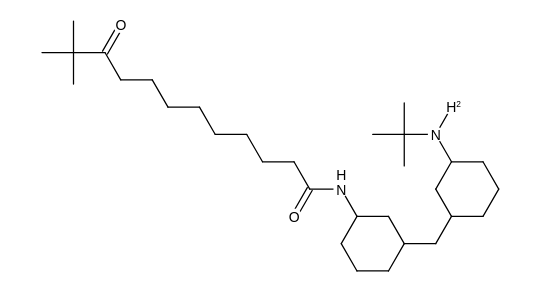
\includegraphics{smile-9130645294707ea727d1c3f6e84a62f199ace142}

Qiana\\
a) Xác định các monomer dùng để tổng hợp Qiana. Phản ứng tổng hợp Qiana thuộc ioại phản ứng gì?\\
b) Tơ Qiana thuộc loại tơ gì? Vải sản xuất từ Qiana có bền trong môi trường acid hoặc base mạnh không? Giải thích.\\
14.14. Poly(ethylene terephthalate) là một polyester có tên viết tắt là PET hay PETE, được ứng dụng rộng rãi làm hộp đựng, chai nhựa, sợi polyester,... PET được điều chế từ terephthalic acid và ethylene glycol bằng phản ứng ester hoá.\\
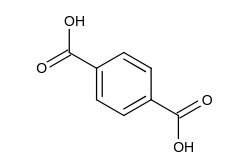
\includegraphics{smile-671cd0ab02d03e9ed4c1bf3aa0b7df9c0ed0d261}

terephthalic acid\\
$\mathrm{HO}-\mathrm{CH}_{2} \mathrm{CH}_{2}-\mathrm{OH}$\\
ethylene glycol\\
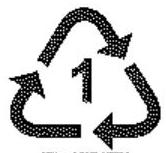
\includegraphics[max width=\textwidth, center]{2025_10_23_74efce88ce3a451fd6b0g-043}

PET\\
kí hiệu nhận dạng\\
a) Viết phương trình hoá học của phản ứng điều chế PET từ các monomer tương ứng. Phản ứng này thuộc loại trùng hợp hay trùng ngưng?\\
b) Từ kí hiệu nhận dạng của nhựa PET, hãy cho biết PET thuộc lại nhựa nhiệt rắn hay nhiệt dẻo và có thể tái chế được hay không?\\
c) Để giảm thiểu tác động tới môi trường, ethylene glycol trước đây được sản xuất từ ethylene có nguồn gốc dầu mỏ được thay thế bằng ethylene sản xuất từ ethanol sinh học (có nguồn gốc từ đường mía). Nhựa PET thu được theo phương pháp này gọi là nhựa PET sinh học (Bio-PET). Viết phương trình hoá học của các phản ứng xảy ra trong quá trình điều chế ethylene glycol từ đường mía.

\section*{Chưong V PIN DIÊN VA ĐIỆN PHÂN}
\section*{BÀI 15}
\section*{THẾ ĐIỆN CỰC VÀ NGUỐN ĐIỆN HOÁ HỌC}
\section*{NHAN BIÉT}
15.1. Mối liên hệ giữa dạng oxi hoá và dạng khử của kim loại M được biểu diễn ở dạng quá trình khử là\\
A. $\mathrm{M} \rightleftharpoons \mathrm{M}^{\mathrm{n}+}+$ ne .\\
B. $\mathrm{M}^{\mathrm{n}+}+\mathrm{ne} \rightleftharpoons \mathrm{M}$.\\
C. $\mathrm{M}^{\mathrm{n}-} \rightleftharpoons \mathrm{M}+$ ne .\\
D. $\mathrm{M}+\mathrm{ne} \rightleftharpoons \mathrm{M}^{\mathrm{n}-}$.\\
15.2. Kí hiệu cặp oxi hoá - khử ứng với quá trình khử: $\mathrm{Fe}^{3+}+1 \mathrm{e} \rightleftharpoons \mathrm{Fe}^{2+}$ là\\
A. $\mathrm{Fe}^{3+} / \mathrm{Fe}^{2+}$.\\
B. $\mathrm{Fe}^{2+} / \mathrm{Fe}$.\\
C. $\mathrm{Fe}^{3+} / \mathrm{Fe}$.\\
D. $\mathrm{Fe}^{2+} / \mathrm{Fe}^{3+}$.\\
15.3. Giá trị thế điện cực chuẩn của cặp oxi hoá - khử nào được quy ước bằng 0 V ?\\
A. $\mathrm{Na}^{+} / \mathrm{Na}$.\\
B. $2 \mathrm{H}^{+} / \mathrm{H}_{2}$.\\
C. $\mathrm{Al}^{3+} / \mathrm{Al}$.\\
D. $\mathrm{Cl}_{2} / 2 \mathrm{Cl}^{-}$.\\
15.4. Cặp oxi hoá - khử nào sau đây có giá trị thế điện cực chuẩn lớn hơn 0 ?\\
A. $\mathrm{K}^{+} / \mathrm{K}$.\\
B. $\mathrm{Li}^{+} / \mathrm{Li}$.\\
C. $\mathrm{Ba}^{2+} / \mathrm{Ba}$.\\
D. $\mathrm{Cu}^{2+} / \mathrm{Cu}$.\\
15.5. Trong số các ion: $\mathrm{Ag}^{+}, \mathrm{Al}^{3+}, \mathrm{Fe}^{2+}, \mathrm{Cu}^{2+}$, ion nào có tính oxi hoá mạnh nhất ở điều kiện chuẩn?\\
A. $\mathrm{Cu}^{2+}$.\\
B. $\mathrm{Fe}^{2+}$.\\
C. $\mathrm{Ag}^{+}$.\\
D. $\mathrm{Al}^{3+}$.\\
15.6. Ở điều kiện chuẩn, Fe khử được ion kim loại nào sau đây trong dung dịch?\\
A. $\mathrm{Mg}^{2+}$.\\
B. $\mathrm{Al}^{3+}$.\\
C. $\mathrm{Na}^{+}$.\\
D. $\mathrm{Ag}^{+}$.\\
15.7. Ở điều kiện chuẩn, kim loại nào sau đây khử được ion $\mathrm{H}^{+}$thành $\mathrm{H}_{2}$ ?\\
A. Mg.\\
B. Cu .\\
C. Hg.\\
D. Au .\\
15.8. Cho các cặp oxi hoá - khử của các kim loại và thế điện cực chuẩn tương ứng:

\begin{center}
\begin{tabular}{|c|c|c|c|c|}
\hline
Cap oxi hoa-khú & $\mathrm{Li}^{+} / \mathrm{Li}$ & $\mathrm{Mg}^{2+} / \mathrm{Mg}$ & $\mathrm{Zn}^{2+} / \mathrm{Zn}$ & $\mathrm{Ag}^{+} / \mathrm{Ag}$ \\
\hline
Thé diên curc chuân, V. & $-3,040$ & $-2,356$ & $-0,762$ & $+0,799$ \\
\hline
\end{tabular}
\end{center}

Trong số các kim loại trên, kim loại có tính khử mạnh nhất là\\
A. Mg.\\
B. Zn .\\
C. Ag.\\
D. Li .\\
15.9. Cho dãy sắp xếp các kim loại theo chiều giảm dần tính khử: $\mathrm{Na}, \mathrm{Mg}, \mathrm{Al}, \mathrm{Fe}$. Trong số các cặp oxi hoá - khử sau, cặp nào có giá trị thế điện cực chuẩn nhỏ nhất?\\
A. $\mathrm{Mg}^{2+} / \mathrm{Mg}$.\\
B. $\mathrm{Fe}^{2+} / \mathrm{Fe}$.\\
C. $\mathrm{Na}^{+} / \mathrm{Na}$.\\
D. $\mathrm{Al}^{3+} / \mathrm{Al}$.\\
15.10. Cho các cặp oxi hoá - khử của các halogen và thế điện cực chuẩn tương ứng:

\begin{center}
\begin{tabular}{|c|c|c|c|c|}
\hline
Cap oxi hod - khur & $\mathrm{F}_{2} / 2 \mathrm{~F}^{-}$ & $\mathrm{Cl}_{2} / 2 \mathrm{Cl}^{-}$ & $\mathrm{Br}_{2} / 2 \mathrm{Br}^{-}$ & $\mathrm{I}_{2} / 2 \mathrm{I}^{-}$ \\
\hline
The dien cure chuán $(V)$ & $+2,87$ & $+1,358$ & $+1,087$ & $+0,621$ \\
\hline
\end{tabular}
\end{center}

Dãy sắp xếp các ion halide theo thứ tự giảm dần tính khử là\\
A. $\mathrm{F}^{-}, \mathrm{Cl}^{-}, \mathrm{Br}^{-}, \mathrm{I}^{-}$.\\
B. $\mathrm{Cl}^{-}, \mathrm{F}^{-}, \mathrm{Br}^{-}, \mathrm{I}^{-}$.\\
C. $\mathrm{I}^{-}, \mathrm{Br}^{-}, \mathrm{Cl}^{-}, \mathrm{F}^{-}$.\\
D. $\mathrm{Br}^{-}, \mathrm{I}^{-}, \mathrm{F}^{-}, \mathrm{Cl}^{-}$.\\
15.11. Trong pin điện hoá $\mathrm{Zn}-\mathrm{Cu}$, phản ứng hoá học xảy ra giữa hai dạng nào của các cặp oxi hoá - khử tương ứng?\\
A. Zn và $\mathrm{Cu}^{2+}$.\\
B. Zn và Cu .\\
C. $\mathrm{Zn}^{2+}$ và $\mathrm{Cu}^{2+}$.\\
D. Zn và $\mathrm{Cu}^{2+}$.\\
15.12. Trong quá trình hoạt động của pin điện $\mathrm{Zn}-\mathrm{Cu}$, dòng electron di chuyển từ\\
A. cực kẽm sang cực đồng.\\
B. cực bên phải sang cực bên trái.\\
C. cathode sang anode.\\
D. cực dương sang cực âm.\\
15.13. Trong quá trình hoạt động của pin điện $\mathrm{Ni}-\mathrm{Cu}$, quá trình xảy ra ở anode là\\
A. $\mathrm{Ni} \rightarrow \mathrm{Ni}^{2+}+2 \mathrm{e}$.\\
B. $\mathrm{Cu} \rightarrow \mathrm{Cu}^{2+}+2 \mathrm{e}$.\\
C. $\mathrm{Cu}^{2+}+2 \mathrm{e} \rightarrow \mathrm{Cu}$.\\
D. $\mathrm{Ni}^{2+}+2 \mathrm{e} \rightarrow \mathrm{Ni}$.\\
15.14. Trong quá trình hoạt động của pin điện $\mathrm{Cu}-\mathrm{Ag}$, điện cực đồng là\\
A. điện cực dương.\\
B. cathode.\\
C. điện cực bị giảm dần khối lượng.\\
D. nơi xảy ra quá trình khử.\\
15.15. Trong quá trình hoạt động của pin điện hoá $\mathrm{Zn}-\mathrm{Cu}$, nhận định về vai trò của cầu muối nào sau đây không đúng?\\
A. Ngăn cách hai dung dịch chất điện li.\\
B. Cho dòng electron chạy qua.\\
C. Trung hoà điện ở mỗi dung dịch điện li.\\
D. Đóng kín mạch điện.

\section*{THONG HIÉU}
15.16. Trong nước, thế điện cực chuẩn của kim loại $\mathrm{M}^{\mathrm{n}+} / \mathrm{M}$ càng nhỏ thì dạng khử có tính khử ...(I)... và dạng oxi hoá có tính oxi hoá ...(II)..... Các cụm từ cần điền vào (I) và (II) lần lượt là\\
A. càng mạnh và càng yếu.\\
B. càng mạnh và càng mạnh.\\
C. càng yếu và càng yếu.\\
D. càng yếu và càng mạnh.\\
15.17. Cho phản ứng hoá học: $\mathrm{Cu}+2 \mathrm{Ag}^{+} \rightarrow \mathrm{Cu}^{2+}+2 \mathrm{Ag}$.

Phát biểu nào sau đây về phản ứng trên là đúng?\\
$\mathrm{A} . \mathrm{Ag}^{+}$khử Cu thành $\mathrm{Cu}^{2+}$.\\
B. $\mathrm{Cu}^{2+}$ có tính oxi hoá mạnh hơn $\mathrm{Ag}^{+}$.\\
$\mathrm{C} . \mathrm{Cu}$ có tính khử yếu hơn Ag .\\
D. Cu là chất khử, $\mathrm{Ag}^{+}$là chất oxi hoá.\\
15.18. Cho các cặp oxi hoá - khử của kim loại và thế điện cực chuẩn tương ứng:

\begin{center}
\begin{tabular}{|l|l|c|c|c|}
\hline
Cap oxi hoa -lau & $\mathrm{Na}^{+} / \mathrm{Na}$ & $\mathrm{Ca}^{2+} / \mathrm{Ca}$ & $\mathrm{Ni}^{2+} / \mathrm{Ni}$ & $\mathrm{Au}^{3+} / \mathrm{Au}$ \\
\hline
Thé dièn cuc chuân $(\mathrm{V})$ & $-2,713$ & $-2,84$ & $-0,257$ & $+1,52$ \\
\hline
\end{tabular}
\end{center}

Trong các kim loại trên, số kim loại tác dụng được với dung dịch HCl ở điều kiện chuẩn, giải phóng khí $\mathrm{H}_{2}$ là\\
A. 1 .\\
B. 4 .\\
C. 2 .\\
D. 3 .\\
15.19. Cho thế điện cực chuẩn của các cặp oxi hoá - khử: $\mathrm{Fe}^{2+} / \mathrm{Fe} ; \mathrm{Na}^{+} / \mathrm{Na} ; \mathrm{Ag}^{+} / \mathrm{Ag}$; $\mathrm{Mg}^{2+} / \mathrm{Mg} ; \mathrm{Cu}^{2+} / \mathrm{Cu}$ lần lượt là $-0,44 \mathrm{~V} ;-2,713 \mathrm{~V} ;+0,799 \mathrm{~V} ;-2,353 \mathrm{~V} ;+0,340 \mathrm{~V}$. Ở điều kiện chuẩn, kim loại Cu khử được ion kim loại nào sau đây?\\
A. $\mathrm{Na}^{+}$.\\
B. $\mathrm{Mg}^{2+}$.\\
C. $\mathrm{Ag}^{+}$.\\
D. $\mathrm{Fe}^{2+}$.\\
15.20. Cho thứ tự sắp xếp một số cặp oxi hoá - khử trong dãy điện hoá:

$$
\mathrm{Al}^{3+} / \mathrm{Al} ; \mathrm{Fe}^{2+} / \mathrm{Fe} ; \mathrm{Sn}^{2+} / \mathrm{Sn} ; \mathrm{Cu}^{2+} / \mathrm{Cu} .
$$

Kim loại nào sau đây có phản ứng với dung dịch muối tương ứng?\\
A. Fe và $\mathrm{CuSO}_{4}$.\\
B. Fe và $\mathrm{Al}_{2}\left(\mathrm{SO}_{4}\right)_{3}$.\\
C. Sn và $\mathrm{FeSO}_{4}$.\\
D. Cu và $\mathrm{SnSO}_{4}$.\\
15.21. Cho thứ tự sắp xếp các cặp oxi hoá - khử trong dãy điện hoá:

$$
\mathrm{Mg}^{2+} / \mathrm{Mg} ; \mathrm{H}_{2} \mathrm{O} / \mathrm{H}_{2} ; \mathrm{OH}^{-} ; 2 \mathrm{H}^{+} / \mathrm{H}_{2} ; \mathrm{Ag}^{+} / \mathrm{Ag} .
$$

Cặp oxi hoá - khử có giá trị thế điện cực chuẩn lớn nhất trong dãy là\\
A. $2 \mathrm{H}^{+} / \mathrm{H}_{2}$.\\
B. $\mathrm{Ag}^{+} / \mathrm{Ag}$.\\
C. $\mathrm{H}_{2} \mathrm{O} / \mathrm{H}_{2}, \mathrm{OH}^{-}$.\\
D. $\mathrm{Mg}^{2+} / \mathrm{Mg}$.\\
15.22. Sức điện động chuẩn của pin điện hoá $\mathrm{H}_{2}-\mathrm{Cu}$ (gồm hai điện cực ứng với hai cặp oxi hoá - khử là $2 \mathrm{H}^{+} / \mathrm{H}_{2}$ và $\mathrm{Cu}^{2+} / \mathrm{Cu}$ ) đo được bằng vôn kế có điện trở vô cùng lớn là $0,340 \mathrm{~V}$. Từ đó, xác định được thế điện cực chuẩn của cặp $\mathrm{Cu}^{2+} / \mathrm{Cu}$ là\\
A. $-0,340 \mathrm{~V}$.\\
B. $0,000 \mathrm{~V}$.\\
C. $0,680 \mathrm{~V}$.\\
D. $+0,340 \mathrm{~V}$.\\
15.23. Thế điện cực chuẩn của các cặp oxi hoá - khử của kim loại $\mathrm{M}^{+} / \mathrm{M}$ và $\mathrm{R}^{2+} / \mathrm{R}$ lần lượt là $+0,799 \mathrm{~V}$ và $+0,34 \mathrm{~V}$. Nhận xét nào sau đây là đúng ở điều kiện chuẩn?\\
A. $M$ có tính khử mạnh hơn $R$.\\
B. $\mathrm{M}^{+}$có tính oxi hoá yếu hơn $\mathrm{R}^{2+}$.\\
C. M khử được ion $\mathrm{H}^{+}$thành $\mathrm{H}_{2}$.\\
D. R khử được ion $\mathrm{M}^{+}$thành M .\\
15.24. Phản ứng hoá học xảy ra trong pin điện hoá $\mathrm{Sn}-\mathrm{Cu}$ :

$$
\mathrm{Sn}+\mathrm{Cu}^{2+} \longrightarrow \mathrm{Sn}^{2+}+\mathrm{Cu}
$$

Trong quá trình hoạt động của pin điện hoá, nhận định nào sau đây là đúng?\\
A. Khối lượng của điện cực Sn tăng.\\
B. Nồng độ $\mathrm{Sn}^{2+}$ trong dung dịch tăng.\\
C. Khối lượng của điện cực Cu giảm.\\
D. Nồng độ $\mathrm{Cu}^{2+}$ trong dung dịch tăng.\\
15.25. Thiết lập pin điện hoá ở điều kiện chuẩn gồm hai điện cực tạo bởi các cặp oxi hoá-khử $\mathrm{Ni}^{2+} / \mathrm{Ni}\left(\mathrm{E}_{\mathrm{Ni}^{2+} / \mathrm{Ni}}^{0}=-0,257 \mathrm{~V}\right)$ và $\mathrm{Cd}^{2+} / \mathrm{Cd}\left(\mathrm{E}_{\mathrm{Cd}^{2+} / \mathrm{Cd}}^{0}=-0,403 \mathrm{~V}\right)$. Sức điện động chuẩn của pin điện hoá trên là\\
A. $+0,146 \mathrm{~V}$.\\
B. $0,000 \mathrm{~V}$.\\
C. $-0,146 \mathrm{~V}$.\\
D. $+0,660 \mathrm{~V}$.\\
15.26. Một pin điện hoá có điện cực Zn nhúng trong dung dịch $\mathrm{ZnSO}_{4}$ và điện cực Cu nhúng trong dung dịch $\mathrm{CuSO}_{4}$. Sau một thời gian pin đó phóng điện thì\\
A. khối lượng điện cực Zn giảm còn khối lượng điện cực Cu tăng.\\
B. khối lượng điện cực Zn tăng còn khối lượng điện cực Cu giảm.\\
C. khối lượng cả hai điện cực Zn và Cu đều tăng.\\
D. khối lượng cả hai điện cực Zn và Cu đều giảm.

Hãy chọn đíng hoặc sai cho mỗi ý $\mathrm{a}, \mathrm{b}, \mathrm{c}, \mathrm{d}$ ở các câu 15.27-15.29.\\
15.27. Trong quá trình một pin Galvani đang hoạt động.\\
a) Năng lượng được chuyển đổi từ hoá năng thành điện năng.\\
b) Xảy ra phản ứng oxi hoá - khử tự diễn biến.\\
c) Quá trình oxi hoá và quá trình khử xảy ra riêng biệt ở hai điện cực.\\
d) Sức điện động của pin không thay đổi theo thời gian.\\
15.28. Xét pin Galvani tạo bởi hai điện cực kim loại:\\
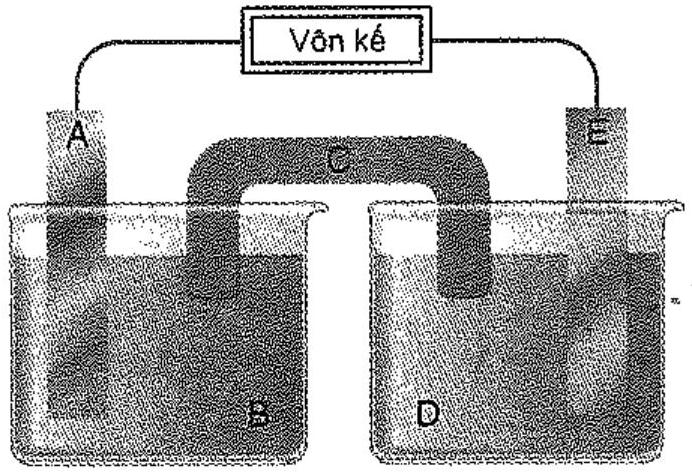
\includegraphics[max width=\textwidth, center]{2025_10_23_74efce88ce3a451fd6b0g-048}\\
a) A là anode, E là cathode, C là cầu muối.\\
b) Nếu A là Zn thì B phải là $\mathrm{ZnSO}_{4}$.\\
c) Nếu C chứa $\mathrm{KNO}_{3}$ thì ion $\mathrm{K}^{+}$được chuyển từ C vào D .\\
d) Chiều dòng điện ở mạch ngoài từ A sang E .\\
15.29. Một pin điện hoá $\mathrm{Zn}-\mathrm{H}_{2}$ được thiết lập ở các điều kiện như hình vẽ sau (vôn kế có điện trở rất lớn).\\
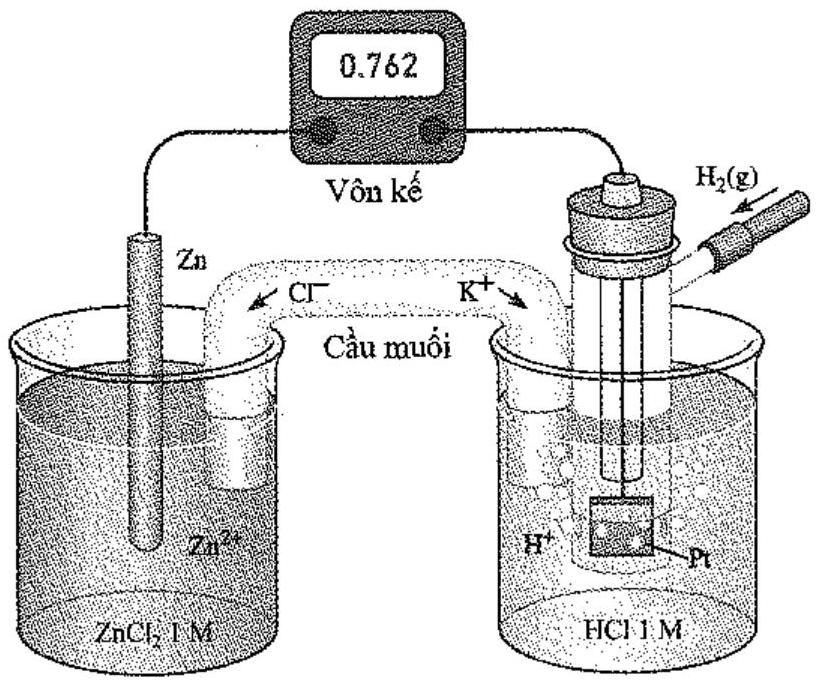
\includegraphics[max width=\textwidth, center]{2025_10_23_74efce88ce3a451fd6b0g-048(1)}\\
a) Giá trị thế điện cực chuẩn của cặp oxi hoá - khử $\mathrm{Zn}^{2+} / \mathrm{Zn}$ là $0,762 \mathrm{~V}$.\\
b) Quá trình khử xảy ra ở cathode là: $2 \mathrm{H}^{+}+2 \mathrm{e} \rightarrow \mathrm{H}_{2}$.\\
c) Chất điện li trong cầu muối là KCl .\\
d) Phản ứng hoá học xảy ra trong pin là: $\mathrm{Zn}+2 \mathrm{H}^{+} \rightarrow \mathrm{Zn}^{2+}+\mathrm{H}_{2}$.\\
15.30. Lắp ráp pin điện hoá $\mathrm{Sn}-\mathrm{Cu}$ ở điều kiện chuẩn. Cho biết các giá trị thế điện cực chuẩn: $\mathrm{E}_{\mathrm{Sn}^{2+} / \mathrm{Sn}}^{\mathrm{o}}=-0,137 \mathrm{~V}$ và $\mathrm{E}_{\mathrm{Cu}^{2+} / \mathrm{Cu}}^{\mathrm{o}}=+0,340 \mathrm{~V}$.\\
Sức điện động chuẩn của pin điện hoá trên là bao nhiêu vôn? (Làm tròn kết quả đến phần trăm.)

\section*{VAN DUNG}
15.31. Một pin điện hoá được thiết lập từ hai điện cực tạo bởi hai cặp oxi hoá - khử là $\mathrm{M}^{2+} / \mathrm{M}$ và $\mathrm{Ag}^{+} / \mathrm{Ag}$. Cho biết:

\begin{center}
\begin{tabular}{|cc|c|c|c|c|}
\hline
Cap oxi hoa -khi & $\mathrm{Fe}^{2+} / \mathrm{Fe}$ & $\mathrm{Ni}^{2+} / \mathrm{Ni}$ & $\mathrm{Sn}^{2+} / \mathrm{Sn}$ & $\mathrm{Cu}^{2+} / \mathrm{Cu}$ & $\mathrm{Ag}^{+} / \mathrm{Ag}$ \\
\hline
Thé dièn cuc chuán $(\mathrm{V})$ & $-0,44$ & $-0,257$ & $-0,137$ & $+0,340$ & $+0,799$ \\
\hline
\end{tabular}
\end{center}

Nếu M là một trong số các kim loại: $\mathrm{Fe}, \mathrm{Ni}, \mathrm{Sn}, \mathrm{Cu}$ thì sức điện động chuẩn lớn nhất của pin bằng bao nhiêu vôn? (Làm tròn kết quả đến phần trăm.)\\
15.32. Cho các cặp oxi hoá - khử và thế điện cực chuẩn tương ứng:

\begin{center}
\begin{tabular}{|cc|c|c|c|}
\hline
Cap oxi hoa-khur & $\mathrm{Cu}^{2+} / \mathrm{Cu}$ & $\mathrm{Zn}^{2+} / \mathrm{Zn}$ & $\mathrm{Fe}^{2+} / \mathrm{Fe}$ & $\mathrm{Ag}^{+} / \mathrm{Ag}$ \\
\hline
Thé dièn cur chuán $(\mathrm{V})$ & $+0,34$ & $-0,762$ & $-0,44$ & $+0,799$ \\
\hline
\end{tabular}
\end{center}

Pin có sức điện động lớn nhất là\\
A. $\operatorname{Pin} \mathrm{Zn}-\mathrm{Cu}$.\\
B. $\mathrm{Pin} \mathrm{Fe}-\mathrm{Cu}$.\\
C. $\operatorname{Pin} \mathrm{Cu}-\mathrm{Ag}$.\\
D. $\mathrm{Pin} \mathrm{Fe}-\mathrm{Ag}$.\\
15.33. Cho các pin điện hoá và sức điện động chuẩn tương ứng:

\begin{center}
\begin{tabular}{|c|c|c|c|}
\hline
Pin dièn hod & $\mathrm{Cu}-\mathrm{X}$ & $\mathrm{Y}-\mathrm{Cu}$ & $\mathrm{Z}-\mathrm{Cu}$ \\
\hline
Sic dièn dóng chuân $(\mathrm{V})$ & 0,46 & 1,1 & 1,47 \\
\hline
\end{tabular}
\end{center}

( $\mathrm{X}, \mathrm{Y}, \mathrm{Z}$ là ba kim loại.)\\
Dãy các kim loại xếp theo chiều tăng dần tính khử từ trái sang phải là\\
A. $\mathrm{X}, \mathrm{Cu}, \mathrm{Z}, \mathrm{Y}$.\\
B. $\mathrm{Y}, \mathrm{Z}, \mathrm{Cu}, \mathrm{X}$.\\
C. Z, Y, Cu, X.\\
D. $\mathrm{X}, \mathrm{Cu}, \mathrm{Y}, \mathrm{Z}$.\\
15.34. Cho các cặp oxi hoá - khử và thế điện cực chuẩn tương ứng:

\begin{center}
\begin{tabular}{|c|c|c|c|c|}
\hline
Cap oxitiod-khu & $\mathrm{Cr}^{2+} / \mathrm{Cr}$ & $\mathrm{Cr}^{3+} / \mathrm{Cr}^{2+}$ & $\mathrm{Zn}^{2+} / \mathrm{Zn}$ & $\mathrm{Ni}^{2+} / \mathrm{Ni}$ \\
\hline
Thé dien eure chuán $(\mathrm{V})$ & $-0,91$ & $-0,41$ & $-0,76$ & $-0,26$ \\
\hline
\end{tabular}
\end{center}

Phản ứng nào sau đây đúng?\\
A. $\mathrm{Zn}+\mathrm{Cr}^{3+} \longrightarrow \mathrm{Zn}^{2+}+\mathrm{Cr}^{2+}$.\\
B. $\mathrm{Zn}+\mathrm{Cr}^{2+} \longrightarrow \mathrm{Zn}^{2+}+\mathrm{Cr}$.\\
C. $\mathrm{Zn}+\mathrm{Cr}^{3+} \longrightarrow \mathrm{Zn}^{2+}+\mathrm{Cr}$.\\
D. $\mathrm{Ni}+\mathrm{Cr}^{3+} \longrightarrow \mathrm{Ni}^{2+}+\mathrm{Cr}^{2+}$.

Hãy chọn đúng hoặc sai cho mỗi ý $a, b, c, d$ ở các câu 15.35-15.36.\\
15.35. Trong một pin điện hoá xảy ra phản ứng sau:

$$
\mathrm{Cu}+2 \mathrm{Fe}^{3+} \longrightarrow \mathrm{Cu}^{2+}+2 \mathrm{Fe}^{2+}
$$

a) Kim loại Cu bị oxi hoá bởi $\mathrm{Fe}^{3+}$.\\
b) Tính khử của Cu lớn hơn tính khử của $\mathrm{Fe}^{2+}$.\\
c) Cathode của pin là điện cực ứng với cặp $\mathrm{Fe}^{3+} / \mathrm{Fe}$.\\
d) Cặp $\mathrm{Cu}^{2+} / \mathrm{Cu}$ có thế điện cực chuẩn lớn hơn cặp $\mathrm{Fe}^{3+} / \mathrm{Fe}^{2+}$.\\
15.36. Trong một pin điện hoá xảy ra phản ứng oxi hoá - khử sau:

$$
\mathrm{Fe}+\mathrm{Ni}^{2+} \longrightarrow \mathrm{Fe}^{2+}+\mathrm{Ni}
$$

a) Thanh Ni là cực dương và xảy ra quá trình khử.\\
b) Các electron chuyển từ thanh Fe sang thanh Ni qua cầu muối.\\
c) Tính oxi hoá của $\mathrm{Ni}^{2+}$ lớn hơn của $\mathrm{Fe}^{2+}$.\\
d) Nồng độ của $\mathrm{Ni}^{2+}$ giảm thì sức điện động của pin cũng giảm.\\
15.37. Cho các pin điện hoá và sức điện động chuẩn tương ứng:

\begin{center}
\begin{tabular}{|l|c|c|c|}
\hline
Pin dien hoa & $\mathrm{Ni}-\mathrm{Sn}$ & $\mathrm{Zn}-\mathrm{Cu}$ & $\mathrm{Sn}-\mathrm{Cu}$ \\
\hline
Súc dien dong chuan $(\mathrm{V})$ & 0,12 & 1,101 & 0,597 \\
\hline
\end{tabular}
\end{center}

Sức điện động chuẩn của pin $\mathrm{Ni}-\mathrm{Zn}$ bằng bao nhiêu? (Làm tròn kết quả đến phần trăm.)\\
15.38. Hai cặp oxi hoá - khử $\mathrm{Ni}^{2+} / \mathrm{Ni}$ và $\mathrm{Cd}^{2+} / \mathrm{Cd}$ tạo thành pin có sức điện động chuẩn là $0,146 \mathrm{~V}$. Phản ứng xảy ra trong pin: $\mathrm{Cd}+\mathrm{Ni}^{2+} \longrightarrow \mathrm{Cd}^{2+}+\mathrm{Ni}$.\\
Thế điện cực chuẩn của cặp $\mathrm{Cd}^{2+} / \mathrm{Cd}$ có giá trị là bao nhiêu vôn? (Làm tròn kết quả đến phần trăm.)\\
(Cho biết: ở trạng thái chuẩn, pin $\mathrm{Ni}-\mathrm{Pb}$ có sức điện động $0,131 \mathrm{~V}$;

$$
\left.\mathrm{E}_{\mathrm{Pb}^{2+} / \mathrm{Pb}}^{\mathrm{O}}=-0,126 \mathrm{~V}\right) .
$$

\section*{BÀI 16}
\section*{ĐIỆN PHÂN}
\section*{NHAN BIST}
16.1. Ion kim loại nào sau đây bị điện phân trong dung dịch (với điện cực graphite)?\\
A. $\mathrm{Na}^{+}$.\\
B. $\mathrm{Cu}^{2+}$.\\
C. $\mathrm{Ca}^{2+}$.\\
D. $\mathrm{K}^{+}$.\\
16.2. Ion halide hầu như không bị điện phân trong dung dịch là\\
A. $\mathrm{Br}^{-}$.\\
B. $\mathrm{I}^{-}$.\\
C. $\mathrm{F}^{-}$.\\
D. $\mathrm{Cl}^{-}$.\\
16.3. Phương trình hoá học nào sau đây biểu diễn quá trình điều chế kim loại bằng phương pháp điện phân nóng chảy?\\
A. $\mathrm{CaCl}_{2} \longrightarrow \mathrm{Ca}+\mathrm{Cl}_{2}$.\\
B. $\mathrm{Fe}_{2} \mathrm{O}_{3}+3 \mathrm{CO} \longrightarrow 2 \mathrm{Fe}+3 \mathrm{CO}_{2}$.\\
C. $\mathrm{Mg}+\mathrm{CuSO}_{4} \longrightarrow \mathrm{MgSO}_{4}+\mathrm{Cu}$.\\
D. $2 \mathrm{NaCl}+2 \mathrm{H}_{2} \mathrm{O} \longrightarrow 2 \mathrm{NaOH}+\mathrm{H}_{2}+\mathrm{Cl}_{2}$.\\
16.4. Phương trình hoá học nào sau đây biểu diễn quá trình điều chế kim loại bằng phương pháp điện phân dung dịch?\\
A. $2 \mathrm{Al}_{2} \mathrm{O}_{3} \longrightarrow 4 \mathrm{Al}+3 \mathrm{O}_{2}$.\\
B. $2 \mathrm{Al}+\mathrm{Cr}_{2} \mathrm{O}_{3} \longrightarrow \mathrm{Al}_{2} \mathrm{O}_{3}+2 \mathrm{Cr}$.\\
C. $\mathrm{Zn}+\mathrm{CuSO}_{4} \longrightarrow \mathrm{ZnSO}_{4}+\mathrm{Cu}$.\\
D. $\mathrm{CuCl}_{2} \longrightarrow \mathrm{Cu}+\mathrm{Cl}_{2}$.\\
16.5. Trong công nghiệp, quá trình điện phân dung dịch NaCl bão hoà (điện cực trơ, có màng ngăn xốp) tạo ra khí nào sau đây ở cathode?\\
A. Hydrogen.\\
B. Chlorine.\\
C. Oxygen.\\
D. Hydrogen chloride.\\
16.6. Khi điện phân dung dịch gồm NaCl 1 M và NaBr 1 M , quá trình oxi hoá đầu tiên xảy ra ở anode là\\
A. $2 \mathrm{H}_{2} \mathrm{O} \rightarrow 4 \mathrm{H}^{+}+\mathrm{O}_{2}+4 \mathrm{e}$.\\
B. $2 \mathrm{Cl}^{-} \rightarrow \mathrm{Cl}_{2}+2 \mathrm{e}$.\\
C. $2 \mathrm{Br}^{-} \rightarrow \mathrm{Br}_{2}+2 \mathrm{e}$.\\
D. $\mathrm{Na} \rightarrow \mathrm{Na}^{+}+1 \mathrm{e}$.\\
16.7. Trong quá trình điện phân dung dịch $\mathrm{CuSO}_{4}$ với anode bằng graphite, ở anode xảy ra quá trình\\
A. $2 \mathrm{H}_{2} \mathrm{O}+2 \mathrm{e} \rightarrow \mathrm{H}_{2}+2 \mathrm{OH}^{-}$.\\
B. $2 \mathrm{H}_{2} \mathrm{O} \rightarrow 4 \mathrm{H}^{+}+\mathrm{O}_{2}+4 \mathrm{e}$.\\
C. $\mathrm{Cu}^{2+}+2 \mathrm{e} \rightarrow \mathrm{Cu}$.\\
D. $\mathrm{Cu} \rightarrow \mathrm{Cu}^{2+}+2 \mathrm{e}$.\\
16.8. Khi điện phân dung dịch gồm $\mathrm{Cu}\left(\mathrm{NO}_{3}\right)_{2} 0,1 \mathrm{M}$ và $\mathrm{AgNO}_{3} 0,1 \mathrm{M}$, quá trình khử đầu tiên xảy ra ở cathode là\\
A. $\mathrm{Ag}^{+}+1 \mathrm{e} \rightarrow \mathrm{Ag}$.\\
B. $\mathrm{Cu}^{2+}+2 \mathrm{e} \rightarrow \mathrm{Cu}$.\\
C. $2 \mathrm{H}_{2} \mathrm{O}+2 \mathrm{e} \rightarrow \mathrm{H}_{2}+2 \mathrm{OH}^{-}$.\\
D. $2 \mathrm{H}^{+}+2 \mathrm{e} \rightarrow \mathrm{H}_{2}$.\\
16.9. Phản ứng hoá học chính xảy ra trong quá trình điện phân nóng chảy $\mathrm{Al}_{2} \mathrm{O}_{3}$ trong $3 \mathrm{NaF} \cdot \mathrm{AlF}_{3}$ là\\
A. $2 \mathrm{AlF}_{3} \longrightarrow 2 \mathrm{Al}+3 \mathrm{~F}_{2}$.\\
B. $2 \mathrm{NaF} \longrightarrow \mathrm{Na}+\mathrm{F}_{2}$.\\
C. $2 \mathrm{H}_{2} \mathrm{O} \longrightarrow 2 \mathrm{H}_{2}+\mathrm{O}_{2}$.\\
D. $2 \mathrm{Al}_{2} \mathrm{O}_{3} \longrightarrow 4 \mathrm{Al}+3 \mathrm{O}_{2}$.\\
16.10. Việc duy trì điện áp thấp ( $\sim 5 \mathrm{~V}$ ) trong quá trình điện phân nóng chảy $\mathrm{Al}_{2} \mathrm{O}_{3}$ trong $3 \mathrm{NaF} \cdot \mathrm{AlF}_{3}$ nhằm ngăn cản quá trình nào sau đây xảy ra ở cathode?\\
A. $\mathrm{Al}^{3+}+3 \mathrm{e} \rightarrow \mathrm{Al}$.\\
B. $\mathrm{Na}^{+}+1 \mathrm{e} \rightarrow \mathrm{Na}$.\\
C. $\mathrm{F}_{2}+2 \mathrm{e} \rightarrow 2 \mathrm{~F}^{-}$.\\
D. $\mathrm{O}_{2}+4 \mathrm{e} \rightarrow 2 \mathrm{O}^{2-}$.\\
16.11. Trong công nghiệp, phương pháp điện phân dung dịch được sử dụng để sản xuất một lượng đáng kể kim loại nào sau đây?\\
A. Zn .\\
B. Al.\\
C. Fe.\\
D. Mg.\\
16.12. Trong công nghiệp, việc tinh chế đồng từ đồng thô được thực hiện bằng phương pháp điện phân dung dịch với anode làm bằng\\
A. graphite.\\
${ }^{4}$ B. platinum.\\
C. thép.\\
D. đồng thô.\\
16.13. Điện phân dung dịch chất nào sau đây (dùng điện cực trơ), thu được dung dịch có khả năng làm quỳ tím chuyển sang màu đỏ?\\
A. NaBr .\\
B. NaCl .\\
C. $\mathrm{CuSO}_{4}$.\\
D. $\mathrm{CuCl}_{2}$.\\
16.14. Điện phân dung dịch chất nào sau đây (với điện cực trơ, không có màng ngăn điện cực), thu được dung dịch có khả năng tấy màu?\\
A. $\mathrm{CuSO}_{4}$.\\
B. NaCl .\\
C. $\mathrm{K}_{2} \mathrm{SO}_{4}$.\\
D. $\mathrm{AgNO}_{3}$.\\
16.15. Trong quá trình mạ bạc cho một chiếc vòng bằng thép thì ở anode xảy ra quá trình\\
A. $\mathrm{Ag} \rightarrow \mathrm{Ag}^{+}+1 \mathrm{e}$.\\
B. $\mathrm{Fe} \rightarrow \mathrm{Fe}^{2+}+2 \mathrm{e}$.\\
C. $2 \mathrm{H}_{2} \mathrm{O} \rightarrow 4 \mathrm{H}^{+}+\mathrm{O}_{2}+4 \mathrm{e}$.\\
D. $\mathrm{C} \rightarrow \mathrm{C}^{4+}+4 \mathrm{e}$.

\section*{THONG HIÉU}
16.16. Xét quá trình điện phân dung dịch $\mathrm{NaCl} 20 \%$ bằng dòng điện một chiều (với điện cực trơ, có màng ngăn xốp). Quá trình khử xảy ra ở cathode là\\
A. $2 \mathrm{H}_{2} \mathrm{O}+2 \mathrm{e} \rightarrow \mathrm{H}_{2}+2 \mathrm{OH}^{-}$.\\
B. $\mathrm{Cl}_{2}+2 \mathrm{e} \rightarrow 2 \mathrm{Cl}^{-}$.\\
C. $2 \mathrm{Cl}^{-} \rightarrow \mathrm{Cl}_{2}+2 \mathrm{e}$.\\
D. $\mathrm{H}_{2} \mathrm{O} \rightarrow 2 \mathrm{H}^{+}+\frac{1}{2} \mathrm{O}_{2}+2 \mathrm{e}$.\\
16.17. Trong quá trình điện phân KCl nóng chảy với các điện cực trơ, ở cathode xảy ra quá trình\\
A. oxi hoá ion $\mathrm{K}^{+}$.\\
B. khử ion $\mathrm{K}^{+}$.\\
C. oxi hoá ion $\mathrm{Cl}^{-}$.\\
D. khử ion $\mathrm{Cl}^{-}$.\\
16.18. Khi điện phân dung dịch gồm $\mathrm{CuSO}_{4} 1,0 \mathrm{M}$ và $\mathrm{H}_{2} \mathrm{SO}_{4} 0,5 \mathrm{M}$, quá trình khử đầu tiên xảy ra ở cathode là\\
A. $2 \mathrm{H}_{2} \mathrm{O}+2 \mathrm{e} \rightarrow \mathrm{H}_{2}+2 \mathrm{OH}^{-}$.\\
B. $\mathrm{Cu}^{2+}+2 \mathrm{e} \rightarrow \mathrm{Cu}$.\\
C. $\mathrm{SO}_{4}^{2}+4 \mathrm{H}^{+}+2 \mathrm{e} \rightarrow \mathrm{SO}_{2}+2 \mathrm{H}_{2} \mathrm{O}$.\\
D. $2 \mathrm{H}^{+}+2 \mathrm{e} \rightarrow \mathrm{H}_{2}$.\\
16.19. Cho các cặp oxi hoá - khử và thế điện cực chuẩn tương ứng:

\begin{center}
\begin{tabular}{|c|c|c|c|c|}
\hline
Cap oxi hoa- kni & $\mathrm{F}_{2} / 2 \mathrm{~F}^{-}$ & $\mathrm{Cl}_{2} / 2 \mathrm{Cl}^{-}$ & $\mathrm{Br}_{2} / 2 \mathrm{Br}^{-}$ & $\mathrm{I}_{2} / 2 \mathrm{I}^{-}$ \\
\hline
Thé dien cure chuán $(\mathrm{V})$ & $+2,87$ & $+1,358$ & $+1,087$ & $+0,621$ \\
\hline
\end{tabular}
\end{center}

Khi điện phân dung dịch chứa đồng thời bốn loại ion halide ở trên với nồng độ mol bằng nhau, ion halide bị điện phân đầu tiên ở anode là\\
A. $\mathrm{Cl}^{-}$.\\
B. $\mathrm{Br}^{-}$.\\
C. $\mathrm{F}^{-}$.\\
D. $\mathrm{I}^{-}$.\\
16.20. Cho các cặp oxi hoá - khử và thế điện cực chuẩn tương ứng:

\begin{center}
\begin{tabular}{|c|c|c|c|c|}
\hline
Cap oxi hoa- kno & $2 \mathrm{H}^{+} / \mathrm{H}_{2}$ & $\mathrm{Cu}^{2+} / \mathrm{Cu}$ & $\mathrm{Fe}^{2+} / \mathrm{Fe}$ & $\mathrm{Ag}^{+} / \mathrm{Ag}$ \\
\hline
The dien curc chuan (Y)) & 0,00 & $+0,34$ & $-0,44$ & $+0,799$ \\
\hline
\end{tabular}
\end{center}

Khi điện phân dung dịch chửa đồng thời bốn loại cation trên với nồng độ mol bằng nhau, cation bị điện phân đầu tiên ở cathode là\\
A. $\mathrm{Cu}^{2+}$.\\
B. $\mathrm{Ag}^{+}$.\\
C. $\mathrm{H}^{+}$.\\
D. $\mathrm{Fe}^{2+}$.\\
16.21. Khi điện phấn dung dịch gồm $\mathrm{Cu}\left(\mathrm{NO}_{3}\right)_{2} 1 \mathrm{M}$ và $\mathrm{AgNO}_{3} 1 \mathrm{M}$, thứ tự điện phân ở cathode là\\
A. $\mathrm{Cu}^{2+}, \mathrm{Ag}^{+}, \mathrm{H}_{2} \mathrm{O}$.\\
B. $\mathrm{Ag}^{+}, \mathrm{Cu}^{2+}, \mathrm{H}_{2} \mathrm{O}$.\\
C. $\mathrm{H}_{2} \mathrm{O}, \mathrm{Cu}^{2+}, \mathrm{Ag}^{+}$.\\
D. $\mathrm{Cu}^{2+}, \mathrm{H}_{2} \mathrm{O}^{+}, \mathrm{Ag}^{+}$.\\
16.22. Khi điện phân dung dịch gồm $\mathrm{CuCl}_{2} 1,0 \mathrm{M}$ và $\mathrm{H}_{2} \mathrm{SO}_{4} 0,5 \mathrm{M}$, thứ tự bị điện phân ở anode là\\
A. $\mathrm{H}_{2} \mathrm{O}, \mathrm{Cl}^{-}$.\\
B. $\mathrm{Cl}^{-}, \mathrm{H}_{2} \mathrm{O}$.\\
C. $\mathrm{SO}_{4}^{2-}, \mathrm{Cl}^{-}, \mathrm{H}_{2} \mathrm{O}$.\\
D. $\mathrm{Cl}^{-}, \mathrm{SO}_{4}^{2-}, \mathrm{H}_{2} \mathrm{O}$.\\
16.23. Khi điện phân dung dịch gồm $\mathrm{CuSO}_{4}$ và HCl (sử dụng điện cực trơ, có màng ngăn xốp), chất khí đầu tiên thoát ra ở anode là\\
A. $\mathrm{O}_{2}$.\\
B. $\mathrm{Cl}_{2}$.\\
C. $\mathrm{H}_{2}$.\\
D. $\mathrm{SO}_{2}$.\\
16.24. Điện phân dung dịch $\mathrm{CuSO}_{4}$ với điện cực trơ. Sau một thời gian, ở cathode thu được $1,28 \mathrm{~g} \mathrm{Cu}$ và ở anode có V mL khí $\mathrm{O}_{2}\left(25^{\circ} \mathrm{C}, 1\right.$ bar ) bay ra.\\
Giá trị của V là\\
A. 495,8 .\\
B. 124,0 .\\
C. 247,9 .\\
D. 743,7 .

Hãy chọn đúng hoăc sai cho mỗi ý $\mathrm{a}, \mathrm{b}, \mathrm{c}, \mathrm{d}$ ở các câu 16.25-16.27.\\
16.25. Trong quá trình điện phân dung dịch $\mathrm{CuSO}_{4}$ với anode bằng đồng.\\
a) Ở anode xảy ra quá trình oxi hoá nước.\\
b) Khối lượng anode không thay đổi.\\
c) Nồng độ $\mathrm{CuSO}_{4}$ trong dung dịch giảm dần.\\
d) Khối lượng cathode tăng.\\
16.26. Điện phân dung dịch NaCl bão hoà (với điện cực trơ, màng ngăn xốp) đến khi nồng độ NaCl giảm đi một nửa thì dừng điện phân.\\
a) Dung dịch sau điện phân làm phenolphthalein chuyển màu hồng.\\
b) Ở cathode chỉ xảy ra quá trình khử ion $\mathrm{Na}^{+}$.\\
c) Số mol khí $\mathrm{Cl}_{2}$ thoát ra ở anode bằng số $\mathrm{mol} \mathrm{H}_{2}$ thoát ra ở cathode.\\
d) Thứ tự điện phân ở anode là $\mathrm{H}_{2} \mathrm{O}, \mathrm{Cl}^{-}$.\\
16.27. Xét quá trình điện phân nóng chảy hợp chất ion MX của kim loại kiềm:\\
a) Cực dương là anode, cực âm là cathode.\\
b) Kim loại M được tạo thành ở cực âm.\\
c) Điện cực âm có dòng electron chuyển đến.\\
d) Cực dương và cực âm nối với các cực tương ứng của nguồn điện.

\section*{VAN DUNG}
16.28. Để mạ $5,0 \mathrm{~g}$ bạc lên một đĩa sắt khi điện phân dung dịch chứa ion $\left[\mathrm{Ag}\left(\mathrm{NH}_{3}\right)_{2}\right]^{+}$ với dòng điện có cường độ $1,5 \mathrm{~A}$ không đổi cần thời gian t phút.\\
Cho biết:

\begin{itemize}
  \item Quá trình khử tại cathode: $\left[\mathrm{Ag}\left(\mathrm{NH}_{3}\right)_{2}\right]^{+}+1 \mathrm{e} \rightarrow \mathrm{Ag}+2 \mathrm{NH}_{3}$.
  \item Điện lượng $\mathrm{q}=\mathrm{It}=\mathrm{n}_{\mathrm{e}} \cdot \mathrm{F}, \mathrm{F}=96500 \mathrm{C} / \mathrm{mol}$.
\end{itemize}

Giá trị của t là bao nhiêu? (Làm tròn kết quả đến phần muời).\\
16.29. Tiến hành điện phân dung dịch $\mathrm{CuSO}_{4}$ với anode bằng đồng. Để hoà tan 100 g đồng ở anode trong 8 giờ thì cần cường độ dòng điện bằng bao nhiêu ampe? (Làm tròn kết quả đến phần mười).\\
16.30. Điện phân 500 mL dung dịch $\mathrm{CuSO}_{4} 0,2 \mathrm{M}$ (điện cực trơ) cho đến khi ở cathode thu được $3,2 \mathrm{~g}$ kim loại thì thể tích khí (đkc) thu được ở anode là\\
A. 1,24 lít.\\
B. 2,48 lít.\\
C. 0,62 lít.\\
D. 3,72 lít.\\
16.31. Điện phân dung dịch $\mathrm{M}\left(\mathrm{NO}_{3}\right)_{\mathrm{n}}$ (điện cực trơ, cường độ dòng điện không đổi), ở cathode chỉ thu được $5,4 \mathrm{~g}$ kim loại M và ở anode thu được 0,31 lít khí (đkc). Kim loại M là\\
A. Fe.\\
B. Cu .\\
C. Ag.\\
D. Pb .

\section*{Hãy chọn đúng hoặc sai cho mỗi ý a, b, c, d ở câu sau.}
16.32. Điện phân dung dịch $\mathrm{MSO}_{4}$ ( M là kim loại) với điện cực trơ, cường độ dòng điện không đồi. Sau thời gian t giây, thu được a mol khí ở anode. Nếu thời gian điện phân là 2 t giây thì tổng số mol khí thu được ở cả hai điện cực là $2,5 \mathrm{a} \mathrm{mol}$. Giả sử hiệu suất điện phân là $100 \%$, khí sinh ra không tan trong nước.\\
a) Tại thời điểm $2 t$ giây, có bọt khí ở cathode.\\
b) Tại thời điểm t giây, ion $\mathrm{M}^{2+}$ chưa bị điện phân hết.\\
c) Dung dịch sau điện phân có $\mathrm{pH}<7$.\\
d) Khi thu được 1,8a mol khí ở anode thì vẫn chưa xuất hiện bọt khí ở cathode.\\
16.33. Điện phân V lít dung dịch $\mathrm{CuCl}_{2} 0,5 \mathrm{M}$ với điện cực trơ. Khi dừng điện phân thu được dung dịch X và 1,86 lít khí $\mathrm{Cl}_{2}$ (đkc) duy nhất ở anode. Toàn bộ dung dịch X tác dụng vừa đủ với $12,6 \mathrm{~g} \mathrm{Fe}$. Giá trị của V là bao nhiêu?\\
16.34. Điện phân 200 mL dung dịch $\mathrm{CuSO}_{4}$ nồng độ $\mathrm{x} \mathrm{mol} / \mathrm{L}$ với điện cực tro. Sau một thời gian thu được dung dịch Y vẫn còn màu xanh, có khối lượng giảm 8 g so với dung dịch ban đầu. Cho $16,8 \mathrm{~g}$ bột sắt vào Y , sau khi các phản ứng xảy ra hoàn toàn, thu được $12,4 \mathrm{~g}$ kim loại. Giá trị của x là bao nhiêu?\\
16.35. Điện phân 500 mL dung dịch $\mathrm{AgNO}_{3}$ với điện cực trơ cho đến khi cathode bắt đầu có khí thoát ra thì dừng. Để trụng hoà dung dịch sau điện phân cần 80 mL dung dịch $\mathrm{NaOH} 0,1 \mathrm{M}$. Biết cường độ dòng điện là $0,2 \mathrm{~A}$, thời gian điện phân là bao nhiêu giây?\\
16.36. Điện phân 500 mL dung dịch X gồm $\mathrm{Cu}\left(\mathrm{NO}_{3}\right)_{2}$ và $\mathrm{AgNO}_{3}$ với cường độ dòng điện $0,804 \mathrm{~A}$ đến khi bọt khí bắt đầu thoát ra ở cathode thì mất 2 giờ, khi đó khối lượng cathode tăng thêm $4,2 \mathrm{~g}$. Nồng độ mol của $\mathrm{Cu}\left(\mathrm{NO}_{3}\right)_{2}$ trong dung dịch X là bao nhiêu?

\section*{BÀI 17}
\section*{ÔN TẬP CHƯONG V}
\section*{NHAN BIÉT}
17.1. Cập oxi hoá - khử nào sau đây có giá trị thế điện cực chuẩn nhỏ hơn 0 ?\\
A. $\mathrm{Ag}^{+} / \mathrm{Ag}$.\\
B. $\mathrm{Na}^{+} / \mathrm{Na}$.\\
C. $\mathrm{Hg}^{2+} / \mathrm{Hg}$.\\
D. $\mathrm{Cu}^{2+} / \mathrm{Cu}$.\\
17.2. Kí hiệu cặp oxi hoá - khử tương ứng với quá trình khử: $\mathrm{Fe}(\mathrm{OH})_{3}+1 \mathrm{e} \rightleftharpoons \mathrm{Fe}(\mathrm{OH})_{2}+\mathrm{OH}^{-}$là\\
A. $\mathrm{Fe}^{3+} / \mathrm{Fe}^{2+}$.\\
B. $\mathrm{Fe}^{2+} / \mathrm{Fe}$.\\
C. $\mathrm{Fe}^{3+} / \mathrm{Fe}$.\\
D. $\mathrm{Fe}(\mathrm{OH})_{3} / \mathrm{Fe}(\mathrm{OH})_{2}$.\\
17.3. Trong dãy điện hoá của kim loại, khi đi từ trái sang phải, tính oxi hoá của các ion kim loại biến đổi như thế nào?\\
A. Không đổi.\\
B. Tuần hoàn.\\
C. Giảm dần.\\
D. Tăng dần.\\
17.4. Trong pin điện hoá $\mathrm{Zn}-\mathrm{Cu}$, ở anode (cực âm) xảy ra quá trình\\
A. oxi hoá Zn thành ion $\mathrm{Zn}^{2+}$.\\
B. khử ion $\mathrm{Cu}^{2+}$ thành Cu .\\
C. khử Cu thành ion $\mathrm{Cu}^{2+}$.\\
D. oxi hoá ion $\mathrm{Zn}^{2+}$ thành Zn .\\
17.5. Khi điện phân dung dịch NaCl bằng dòng điện một chiều (với điện cực trơ, có màng ngăn xốp) thì ở cathode xảy ra quá trình\\
A. oxi hoá $\mathrm{H}_{2} \mathrm{O}$ thành $\mathrm{H}^{+}$và $\mathrm{O}_{2}$.\\
B. khử $\mathrm{Cl}^{-}$thành $\mathrm{Cl}_{2}$.\\
C. oxi hoá $\mathrm{Cl}^{-}$thành $\mathrm{Cl}_{2}$.\\
D. khử $\mathrm{H}_{2} \mathrm{O}$ thành $\mathrm{H}_{2}$ và $\mathrm{OH}^{-}$.\\
17.6. Khi điện phân dung dịch $\mathrm{CuSO}_{4}$ bằng dòng điện một chiều (với điện cực anode bằng Cu ) thì ở anode xảy ra quá trình\\
A. oxi hoá $\mathrm{H}_{2} \mathrm{O}$ thành $\mathrm{H}^{+}$và $\mathrm{O}_{2}$.\\
B. khử $\mathrm{Cu}^{2+}$ thành Cu .\\
C. oxi hoá Cu thành $\mathrm{Cu}^{2+}$.\\
D. khử $\mathrm{H}_{2} \mathrm{O}$ thành $\mathrm{H}_{2}$ và $\mathrm{OH}^{-}$.\\
17.7. Trong nước, thế điện cực chuẩn của kim loại $\mathrm{M}^{\mathrm{n}+} / \mathrm{M}$ càng lớn thì dạng khử có tính khử ...(1) ... và dạng oxi hoá có tính oxi hoá ...(2) ... Cụm từ cần điền vào (1) và (2) lần lượt là\\
A. càng mạnh và càng yếu.\\
B. càng mạnh và càng mạnh.\\
C. càng yếu và càng yếu.\\
D. càng yếu và càng mạnh.

\section*{THONG HEU}
17.8. Cho thứ tự sắp xếp các cặp oxi hoá - khử trong dãy điện hoá:

$$
\mathrm{Mg}^{2+} / \mathrm{Mg} ; \mathrm{H}_{2} \mathrm{O} / \mathrm{H}_{2}, \mathrm{OH}^{-} ; 2 \mathrm{H}^{+} / \mathrm{H}_{2} ; \mathrm{Ag}^{+} / \mathrm{Ag} .
$$

Thí nghiệm nào sau đây không xảy ra phản ứng ở điều kiện chuẩn?\\
A. Cho sợi phoi bào Mg vào nước.\\
B. Cho lá Mg vào dung dịch HCl .\\
C. Cho lá Ag vào dung dịch $\mathrm{H}_{2} \mathrm{SO}_{4}$.\\
D. Cho sợi Mg vào dung dịch $\mathrm{AgNO}_{3}$.\\
17.9. Xét phản ứng hoá học giữa hai cặp oxi hoá - khử của kim loại:

$$
\mathrm{R}+2 \mathrm{M}^{+} \longrightarrow \mathrm{R}^{2+}+2 \mathrm{M}
$$

Biết giá trị thế điện cực chuẩn các cặp oxi hoá - khử $\mathrm{M}^{+} / \mathrm{M}$ và $\mathrm{R}^{2+} / \mathrm{R}$ lần lượt là $x(V)$ và $y(V)$. Nhân xét nào sau đây đúng?\\
A. $x<y$.\\
B. $x>y$.\\
C. $x=y$.\\
D. $2 x=y$.\\
17.10. Cho phản ứng hoá học: $\mathrm{Cu}+2 \mathrm{Fe}^{3+} \longrightarrow \mathrm{Cu}^{2+}+2 \mathrm{Fe}^{2+}$.

Phát biểu nào sau đây về phản ứng trên không đúng?\\
A. Cu bị $\mathrm{Fe}^{3+}$ oxi hoá thành $\mathrm{Cu}^{2+}$.\\
B. $\mathrm{Cu}^{2+}$ có tính oxi hoá mạnh hơn $\mathrm{Fe}^{3+}$.\\
C. $\mathrm{Fe}^{3+}$ bị Cu khử thành $\mathrm{Fe}^{2+}$.\\
D. Cu là chất khử, $\mathrm{Fe}^{3+}$ là chất oxi hoá.\\
17.11. Cho các cặp oxi hoá - khử và thế điện cực chuẩn tương ứng:

\begin{center}
\begin{tabular}{|l|l|c|c|c|}
\hline
Cap oxi hoá -khur & $\mathrm{Na}^{+} / \mathrm{Na}$ & $\mathrm{Mg}^{2+} / \mathrm{Mg}$ & $\mathrm{Al}^{3+} / \mathrm{Al}$ & $\mathrm{Cu}^{2+} / \mathrm{Cu}$ \\
\hline
Thé dien cuo chuán ( V ) & $-2,713$ & $-2,356$ & $-1,676$ & $+0,340$ \\
\hline
\end{tabular}
\end{center}

Ion kim loại nào sau đây bị khử tại cathode khi điện phân (với điện graphite) dung dịch muối sulfate tương ứng?\\
A. $\mathrm{Mg}^{2+}$.\\
B. $\mathrm{Na}^{+}$.\\
C. $\mathrm{Cu}^{2+}$.\\
D. $\mathrm{Al}^{3+}$.

Hãy chọn đúng hoặc sai cho mỗi ý $\mathrm{a}, \mathrm{b}, \mathrm{c}, \mathrm{d}$ ở các câu 17.12-17.13.\\
17.12. Ở điều kiện chuẩn, cho bột Cu dư vào dung dịch $\mathrm{Fe}_{2}\left(\mathrm{SO}_{4}\right)_{3}$ tới khi phản ứng hoàn toàn, thu được chất rắn X và dung dịch Y .\\
Cho biết:

\begin{center}
\begin{tabular}{|c|c|c|c|}
\hline
Cap oxi hoá - khú & $\mathrm{Fe}^{2+} / \mathrm{Fe}$ & $\mathrm{Cu}^{2+} / \mathrm{Cu}$ & $\mathrm{Fe}^{3+} / \mathrm{Fe}^{2+}$ \\
\hline
Thé dièn cuc chuân $(\mathrm{V})$ & $-0,44$ & $+0,340$ & $+0,771$ \\
\hline
\end{tabular}
\end{center}

a) X gồm hai kim loại.\\
b) Cu có tính khử mạnh hơn $\mathrm{Fe}^{2+}$ ở điều kiện chuẩn.\\
c) Y gồm hai chất tan là $\mathrm{CuSO}_{4}$ và $\mathrm{FeSO}_{4}$.\\
d) Trong điều kiện $\mathrm{Fe}_{2}\left(\mathrm{SO}_{4}\right)_{3}$ dư thì Y gồm ba muối.\\
17.13. a) Kim loại càng mạnh thì thế điện cực chuẩn càng âm.\\
b) Khi tạo thành pin điện hoá, kim loại mạnh hơn sẽ đóng vai trò là cathode.\\
c) Điện phân dung dịch $\mathrm{CuSO}_{4}$, cứ thu được 1 mol Cu thì khối lượng dung dịch giảm 80 g .\\
d) Để bảo vệ đồ vật bằng kim loại, nên gắn chúng với những mảnh kim loại yếu hơn.

\section*{VAN DUNG}
\section*{Hãy chọn đúng hoăc sai cho mỗi ý $a, b, c, d$ ở câu sau.}
17.14. Xét quá trình hoạt động của một pin điện hoá $\mathrm{Cu}-\mathrm{Ag}_{4}$ được thiết lập ở các điều kiện như hình vẽ bên.\\
Cho thế điện cực chuẩn của các cặp $\mathrm{Cu}^{2+} / \mathrm{Cu}$ và $\mathrm{Ag}^{+} / \mathrm{Ag}$ lần lượt là $+0,340 \mathrm{~V}$ và $+0,799 \mathrm{~V}$.\\
a) Giá trị sức điện động chuẩn của pin điện hoá trên là $0,459 \mathrm{~V}$.\\
b) Ở anode xảy ra quá trình oxi hoá Cu ,\\
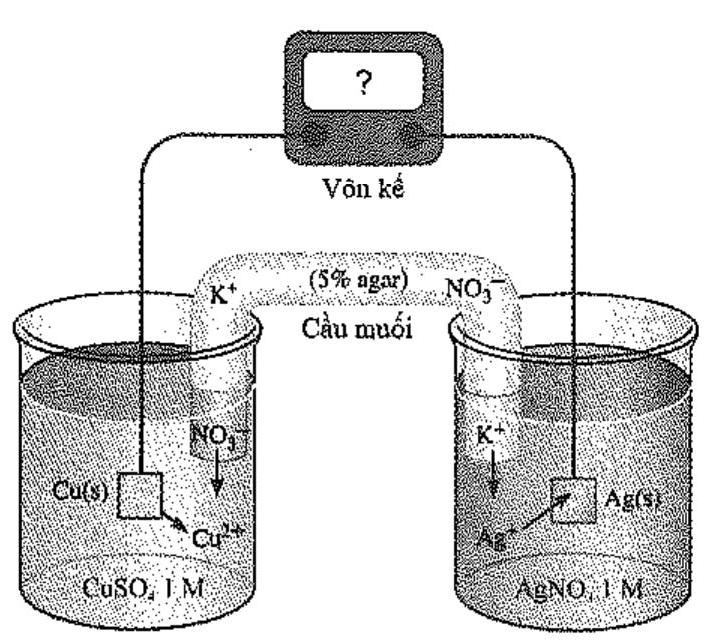
\includegraphics[max width=\textwidth, center]{2025_10_23_74efce88ce3a451fd6b0g-058}\\
ở cathode xảy ra quá trình khử $\mathrm{Ag}^{+}$.\\
c) Điện cực Cu tăng khối lượng, điện cực Ag giảm khối lượng.\\
d) Phản ứng hoá học xảy ra trong pin: $\mathrm{Cu}+2 \mathrm{Ag}^{+} \longrightarrow \mathrm{Cu}^{2+}+2 \mathrm{Ag}$.\\
17.15. Một pin Galvani được lắp ghép từ hai điện cực tạo bởi hai cặp oxi hoá - khử là $\mathrm{Pb}^{2+} / \mathrm{Pb}\left(\mathrm{E}_{\mathrm{Pb}^{2+} / \mathrm{Pb}}^{\mathrm{o}}=-0,126 \mathrm{~V}\right)$ và $\mathrm{Fe}^{3+} / \mathrm{Fe}^{2+}\left(\mathrm{E}_{\mathrm{Fe}^{3+} / \mathrm{Fe}^{2+}}=+0,771 \mathrm{~V}\right)$.\\
Sức điện động chuẩn của pin Galvani trên là bao nhiêu vôn? (Làm tròn kết quả đến phần trăm).\\
17.16. Sức điện động chuẩn của một pin Galvani (được lắp ghép từ hai điện cực tạo bởi hai cặp oxi hoá - khử là $2 \mathrm{H}^{+} / \mathrm{H}_{2}$ và $\mathrm{Ag}^{+} / \mathrm{Ag}$ ) đo được bằng vôn kế có điện trở vô cùng lớn là $0,771 \mathrm{~V}$.\\
Từ kết quả trên, xác định được thế điện cực chuẩn của cặp $\mathrm{Ag}^{+} / \mathrm{Ag}$ là bao nhiêu vôn? (Làm tròn kết quả đến phần trăm).\\
17.17. Điện phân 2 lít dung dịch $\mathrm{NaCl} 0,5 \mathrm{M}$ với điện cực trơ, màng ngăn xốp bằng dòng điện có cường độ không đổi $0,2 \mathrm{~A}$. Sau 1930 giây thì dừng điện phân, thu được dung dịch X (giả thiết thể tích dung dịch không đồi). Dung dịch X có pH bằng bao nhiêu?

\section*{Chưong VI DAI CUONG VÊTIM LOAI}
\section*{BÀl 18}
\section*{CẤU TAO VÀ LIÊN KẾT TRONG TINH THỂ KIM LOAI}
\section*{NHAN BIÉT}
18.1. Cho biết số thứ tự của Mg trong bảng tuần hoàn là 12 . Vị trí của Mg trong bảng tuần hoàn là\\
A. chu kì 3, nhóm IIIA.\\
B. chu kì 3, nhóm IIB.\\
C. chu kì 3 , nhóm IIIA.\\
D. chu kì 2 , nhóm IIA.\\
18.2. Cho biết số thứ tự của Al trong bảng tuần hoàn là 13. Số electron ở lớp ngoài cùng của Al là\\
A. 1 .\\
B. 2 .\\
C. 3 .\\
D. 4 .\\
18.3. Hình vẽ nào sau đây có thể được sử dụng để mô tả cấu trúc tinh thể kim loại?\\
A.\\
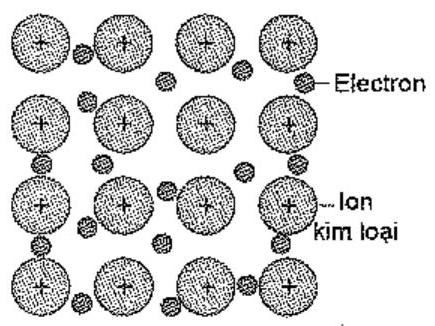
\includegraphics[max width=\textwidth, center]{2025_10_23_74efce88ce3a451fd6b0g-059(3)}\\
B.\\
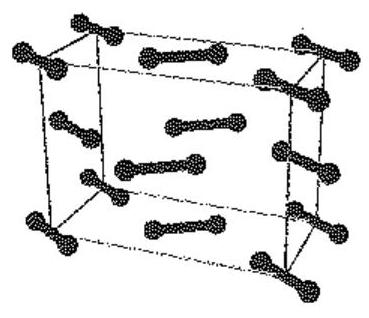
\includegraphics[max width=\textwidth, center]{2025_10_23_74efce88ce3a451fd6b0g-059(2)}\\
C.\\
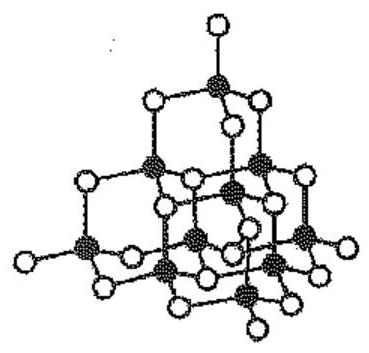
\includegraphics[max width=\textwidth, center]{2025_10_23_74efce88ce3a451fd6b0g-059}\\
D.\\
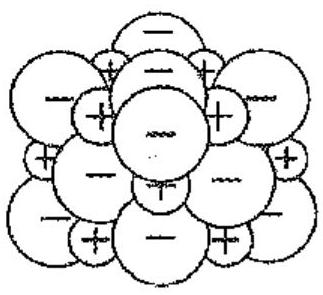
\includegraphics[max width=\textwidth, center]{2025_10_23_74efce88ce3a451fd6b0g-059(1)}\\
18.4. Trong định nghĩa về liên kết kim loại : "Liên kết kim loại là liên kết hình thành do lực hút tĩnh điện giữa các electron ...(1)... với các ion ...(2)... kim loại ở các nút mạng.\\
Các từ cần điền vào vị trí (1), (2) lần lượt là\\
A. ngoài cùng, dương.\\
B. tự do, dương.\\
C. hoá trị, lưỡng cực.\\
D. hoá trị, âm.

\section*{THONG HIÉU}
18.5. Những tính chất vật lí chung của kim loại (dẫn điện, dẫn nhiệt, dẻo, ánh kim) gây nên chủ yếu bởi\\
A. các electron tự do trong tinh thể kim loại.\\
B. kiểu cấu tạo mạng tinh thể của kim loại.\\
C. khối lượng riêng của kìm loại.\\
D. tính chất của kim loại.\\
18.6. Cho các phát biểu sau đây về vị trí và cấu tạo của kim loại:\\
(1) Hầu hết các kim loại chỉ có từ 1 electron đến 3 electron lớp ngoài cùng.\\
(2) Tất các các nguyên tố phân nhóm $B$ (phân nhóm phụ) đều là kim loại.\\
(3) Ở trạng thái rắn, đơn chất kim loại có cấu tạo tinh thể.\\
(4) Các kim loại đều có bán kính nhỏ hơn các phi kim thuộc cùng một chu kì.\\
(5) Liên kết kim loại là liên kết được hình thành giữa các nguyên tử và ion dương kim loại trong mạng tinh thể do sự tham gia của các electron tự do. Những phát biểu đúng là\\
A. (1), (2), (3), (5).\\
B. (1), (2), (3), (4), (5).\\
C. (1), (2), (3).\\
D. (1), (3), (5).

Câu 18.7. Phát biểu nào sau đây đúng?\\
Trong tinh thể kim loại:\\
A. các ion dương kim loại nằm ở các nút mạng tinh thể và các electron hoá trị chuyển động tự do xung quanh.\\
B. các electron hoá trị ở các nút mạng và các ion dương kim loại chuyển động tự do.\\
C. các electron hoá trị và các ion dương kim loại đều chuyển động tự do trong toàn bộ mạng tinh thể.\\
D. các electron hoá trị nằm ở giữa các nguyên tử kim loại cạnh nhau.

Câu 18.8. Phát biểu nào sau đây đúng?\\
Trong tinh thể kim loại, liên kết kim loại được hình thành do\\
A. sự góp chung electron của các nguyên tử kim loại cạnh nhau.\\
B. lực hứt tĩnh điện giữa các electron hoá trị ở các nút mạng với các ion dương kim loại chuyển động tự do.\\
C. lực hút tĩnh điện giữa các electron hoá trị tự do với các ion dương kim loại chuyển động tự do trong toàn bộ mạng tinh thể.\\
D. lực hút tĩnh điện giữa các electron hoá trị tự do với các ion dương kim loại ở các nút mạng.

\section*{VAN DUNG}
Hãy chọn đúng hoăc sai cho mỗi ý $\mathrm{a}, \mathrm{b}, \mathrm{c}, \mathrm{d}$ ỏ các câu $18.9-18.11$.\\
18.9. a) Nguyên tử kim loại thường có 1,2 hoặc 3 electron ở lớp ngoài cùng.\\
b) Trong bảng tuần hoàn, các nhóm A bao gồm các nguyên tố s và nguyên tố p .\\
c) Trong một chu kì, kim loại có bán kính nguyên tử nhỏ hơn phi kim.\\
d) Kim loại có ánh kim do các electron tự do phản xạ ánh sáng nhìn thấy được.\\
18.10. a) Nguyên tử của hầu hết các nguyên tố kim loại đều có ít electron ở lớp ngoài cùng.\\
b) Những tính chất vật lí chung của kim loại chủ yếu do các electron tự do trong mạng tinh thể kim loại gây ra.\\
c) Tính chất hoá học chụng của kim loại là tính oxi hoá.\\
d) Nguyên tắc điều chế kim loại là khử ion kim loại thành nguyên tử.\\
18.11. a) Liên kết kim loại và liên kết cộng hoá trị đều có sự tham gia của các electron.\\
b) Liên kết kim loại khác với liên kết cộng hoá trị ở số electron dùng chung.\\
c) Liên kết kim loại và liên kết ion đều sinh ra bởi lực hút tĩnh điện.\\
d) Liên kết kim loại khác với liên kết ion ở loại hạt mang điện tham gia.

\section*{BÀI 19}
\section*{TÍNH CHẤT VẬT LÍ VÀ TÍNH CHẤT HOÁ HỌC CỦA KIM LOAI}
\section*{NHAN BIÉT}
19.1. Dãy kim loại nào sau đây sắp xếp theo thứ tự độ dẫn điện giảm dần?\\
A. $\mathrm{Au}, \mathrm{Ag}, \mathrm{Cu}, \mathrm{Al}$.\\
B. $\mathrm{Ag}, \mathrm{Au}, \mathrm{Al}, \mathrm{Cu}$.\\
C. $\mathrm{Cu}, \mathrm{Al}, \mathrm{Ag}, \mathrm{Au}$.\\
D. $\mathrm{Ag}, \mathrm{Cu}, \mathrm{Au}, \mathrm{Al}$.\\
19.2. Dây điện cao thế thường được làm bằng nhôm là do nhôm\\
A. là kim loại dẫn điện tốt và nhẹ.\\
B. là kim loại dẫn điện tốt nhất.\\
C. có giá thành rẻ.\\
D. có tính trơ về mặt hoá học.\\
19.3. Khi lựa chọn kim loại để làm vỏ hộp kim loại nhẹ chứa nước ngọt hoặc bia, tính chất nào sau đây thường không được xét đến?\\
A. Tính độc.\\
B. Khối lượng riêng.\\
C. Tính dễ dát mỏng.\\
D. Nhiệt độ nóng chảy.\\
19.4. Ứng dụng nào dưới đây là ứng dụng phổ biến của đồng?\\
A. Làm những bộ phận cấy ghép vào cơ thể người.\\
B. Chế tạo thân máy bay siêu thanh.\\
C. Làm đồ trang sức.\\
D. Làm lõi dây dẫn điện.\\
19.5. Trong trường hợp phải sử dụng kim loại làm đường ống dẫn nước, kim loại nào sau đây là phù hợp nhất để làm đường ống dẫn nước?\\
A. Kẽm.\\
B. Sắt.\\
C. Chì.\\
D. Đồng.\\
19.6. Kim loại nào sau đây không phản ứng với dung dịch HCl loãng?\\
A. Đồng.\\
B. Calcium.\\
C. Magnesium .\\
D. Kẽm.

Hãy chọn đúng hoạc sai cho mỗi ý a, b, c, d ở các câu 19.7-19.8.\\
19.7. a) Kim loại có tính dẫn điện tốt nhất là bạc ( Ag ).\\
b) Kim loại có nhiệt độ nóng chảy thấp nhất là lithium (Li).\\
c) Kim loại có độ cứng lớn nhất là tungsten (W).\\
d) Kim loại nhôm (Al) có thể kéo dài, dát mỏng tốt.\\
19.8. a) Kim loại sắt (dư) cháy trong khí chlorine chỉ tạo một muối.\\
b) Kim loại nhôm có thể tan trong dung dịch kiềm.\\
c) Nhúng thanh Zn vào dung dịch $\mathrm{CuSO}_{4}$ thì khối lượng thanh Zn tăng.\\
d) Kim loại $\mathrm{Al}, \mathrm{Fe}$ đều không tan trong dung dịch $\mathrm{H}_{2} \mathrm{SO}_{4}$ đặc, nguội.

\section*{-2 THONG HIEU}
19.9. Tiến hành các thí nghiệm sau:\\
(1) Cho Mg vào lượng dư dung dịch $\mathrm{FeCl}_{3}$.\\
(2) Cho Ba vào dung dịch $\mathrm{CuSO}_{4}$.\\
(3) Cho Zn vào dung dịch $\mathrm{CuSO}_{4}$.\\
(4) Cho dung dịch $\mathrm{Fe}\left(\mathrm{NO}_{3}\right)_{2}$ vào dung dịch $\mathrm{AgNO}_{3}$.

Thí nghiệm nào thu được kim loại?\\
19.10. Cho bột Fe vào dung dịch gồm $\mathrm{AgNO}_{3}$ và $\mathrm{Cu}\left(\mathrm{NO}_{3}\right)_{2}$. Sau khi các phản ứng xảy ra hoàn toàn, thu được dung dịch X gồm hai muối và chất rắn Y gồm hai kim loại. Hai muối trong X và hai kim loại trong Y lần lượt là:\\
A. $\mathrm{Cu}\left(\mathrm{NO}_{3}\right)_{2} ; \mathrm{Fe}\left(\mathrm{NO}_{3}\right)_{2}$ và $\mathrm{Cu} ; \mathrm{Fe}$.\\
B. $\mathrm{Cu}\left(\mathrm{NO}_{3}\right)_{2} ; \mathrm{Fe}\left(\mathrm{NO}_{3}\right)_{2}$ và $\mathrm{Ag} ; \mathrm{Cu}$.\\
C. $\mathrm{Fe}\left(\mathrm{NO}_{3}\right)_{2} ; \mathrm{Fe}\left(\mathrm{NO}_{3}\right)_{3}$ và $\mathrm{Cu} ; \mathrm{Ag}$.\\
D. $\mathrm{Cu}\left(\mathrm{NO}_{3}\right)_{2} ; \mathrm{AgNO}_{3}$ và $\mathrm{Cu} ; \mathrm{Ag}$.\\
19.11. Cho $0,02 \mathrm{~mol} \mathrm{Na}$ vào 1000 mL dung dịch chứa $\mathrm{CuSO}_{4} 0,05 \mathrm{M}$ và $\mathrm{H}_{2} \mathrm{SO}_{4} 0,005 \mathrm{M}$. Hiện tượng của thí nghiệm trên là\\
A. có khí bay lên và có kết tủa màu xanh lam.\\
B. chỉ có khí bay lên.\\
C. chỉ có kết tủa màu xạnh lam.\\
D. có khí bay lên và có kết tủa sau đó kết tủa tan.\\
19.12. Kẽm khử được các cation kim loại trong dãy muối nào sau đây?\\
A. $\mathrm{Cu}\left(\mathrm{NO}_{3}\right)_{2}, \mathrm{~Pb}\left(\mathrm{NO}_{3}\right)_{2}, \mathrm{Ni}\left(\mathrm{NO}_{3}\right)_{2}$.\\
B. $\mathrm{AlCl}_{3}, \mathrm{MgCl}_{2}, \mathrm{~Pb}\left(\mathrm{NO}_{3}\right)_{2}$.\\
C. $\mathrm{AlCl}_{3}, \mathrm{Ni}\left(\mathrm{NO}_{3}\right)_{2}, \mathrm{~Pb}\left(\mathrm{NO}_{3}\right)_{2}$.\\
D. $\mathrm{MgCl}_{2}, \mathrm{NaCl}, \mathrm{Cu}\left(\mathrm{NO}_{3}\right)_{2}$.\\
19.13. Tiến hành 2 thí nghiệm sau:

\begin{itemize}
  \item Thí nghiệm 1: cho m gam bột $\mathrm{Fe}(\mathrm{du})$ vào $\mathrm{V}_{1}$ lít dung dịch $\mathrm{Cu}\left(\mathrm{NO}_{3}\right)_{2} 1 \mathrm{M}$.
  \item Thí nghiệm 2: cho $m$ gam bột Fe (dư) vào $\mathrm{V}_{2}$ lít dung dịch $\mathrm{AgNO}_{3} 0,1 \mathrm{M}$. Sau khi các phản ứng xảy ra hoàn toàn, khối lượng chất rắn thu được ở hai thí nghiệm đều bằng nhau. Giá trị của $\mathrm{V}_{1}$ so với $\mathrm{V}_{2}$ là\\
A. $\mathrm{V}_{1}=\mathrm{V}_{2}$.\\
B. $\mathrm{V}_{1}=10 \mathrm{~V}_{2}$.\\
C. $\mathrm{V}_{1}=5 \mathrm{~V}_{2}$.\\
D. $\mathrm{V}_{1}=2 \mathrm{~V}_{2}$.\\
19.14. Cho m gam hỗn hợp X gồm Mg và Zn vào dung dịch $\mathrm{H}_{2} \mathrm{SO}_{4}$ loãng, dư thu được 0,7437 lít $\mathrm{H}_{2}$ (đkc). Khi cho m gam hỗn hợp X vào 200 mL dung dịch chứa $\mathrm{CuSO}_{4} 0,2 \mathrm{M}$ thì thu được bao nhiêu gam kết tủa?\\
19.15. Nung nóng hỗn hợp X gồm $3,36 \mathrm{~g}$ bột sắt và $1,28 \mathrm{~g}$ bột lưu huỳnh (không có không khí), thu được hỗn hợp Y . Hoà tan Y vào dung dịch HCl dư, thu được hỗn hợp khí Z. Đốt cháy Z cần a mol oxygen. Giá trị của a là bao nhiêu? (Biết các phản ứng xảy ra hoàn toàn).\\
19.16. Hoà tan hoàn toàn $10,4 \mathrm{~g}$ hỗn hợp $\mathrm{Mg}, \mathrm{Al}$ và Zn trong dung dịch HCl dư, thu được 7,437 lít khí $\mathrm{H}_{2}$ (đkc) và dung dịch chứa m gam muối. Giá trị của m là bao nhiêu?
\end{itemize}

\section*{VAN DUNG}
19.17. Nhúng một thanh Zn vào 100 mL dung dịch $\mathrm{CuSO}_{4}$, sau một thời gian phản ứng lấy thanh Zn ra khỏi dung dịch, làm khô và đem cân thấy khối lượng thanh Zn giảm $0,01 \mathrm{~g}$. Cho dung dịch loãng NaOH dư vào dung dịch sau phản ứng thu được $0,49 \mathrm{~g}$ kết tủa. Nồng độ mol của dung dịch $\mathrm{CuSO}_{4}$ ban đầu là\\
A. $0,15 \mathrm{M}$.\\
B. $0,015 \mathrm{M}$.\\
C. $0,1 \mathrm{M}$.\\
D. $0,05 \mathrm{M}$.\\
19.18. Cho $0,35 \mathrm{~mol}$ hỗn hợp X gồm $\mathrm{Cl}_{2}$ và $\mathrm{O}_{2}$ phản ứng vừa đủ với $11,1 \mathrm{~g}$ hỗn hợp Y gồm Mg và Al , thu được $30,1 \mathrm{~g}$ hỗn hợp Z . Phần trăm khối lượng của Al trong Y là\\
A. $75,68 \%$.\\
B. $24,32 \%$.\\
C. $51,35 \%$.\\
D. $48,65 \%$.\\
19.19. Cho $0,456 \mathrm{~g}$ hỗn hợp bột Fe và Al vào 250 mL dung dịch $\mathrm{AgNO}_{3} 0,12 \mathrm{M}$. Sau khi các phản ứng xảy ra hoàn toàn, thu được dung dịch X và $3,312 \mathrm{~g}$ chất rắn. Khối lượng Fe trong hỗn hợp ban đầu là bao nhiêu gam?\\
19.20. Nung nóng $11,9 \mathrm{~g}$ hỗn hợp $\mathrm{Mg}, \mathrm{Al}$ và Fe trong không khí một thời gian, thu được $13,5 \mathrm{~g}$ hỗn hợp rắn X . Hoà tan vừa đủ X trong V mL dung dịch HCl 1 M , thu được 7,437 lít khí $\mathrm{H}_{2}$ (đkc) và dung dịch chỉ chứa muối. Giá trị của V là bao nhiêu?\\
19.21. Cho hỗn hợp X gồm Al và Mg tác dụng với 200 mL dung dịch gồm $\mathrm{AgNO}_{3}$ a $\mathrm{mol} / \mathrm{L}$ và $\mathrm{Cu}\left(\mathrm{NO}_{3}\right)_{2} 2 \mathrm{a} \mathrm{mol} / \mathrm{L}$, thu được $9,04 \mathrm{~g}$ chất rắn Y . Cho Y tác dụng với dung dịch $\mathrm{H}_{2} \mathrm{SO}_{4}$ đặc, nóng (dư), thu được 1,7353 lít khí $\mathrm{SO}_{2}$ (ở đlkc, là sản phẩm khử duy nhất). Giá trị của a là bao nhiêu? (Biết các phản ứng xảy ra hoàn toàn).\\
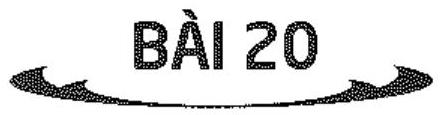
\includegraphics[max width=\textwidth, center]{2025_10_23_74efce88ce3a451fd6b0g-065}

\section*{NHAN BIET}
20.1. Chất nào dưới đây là thành phần chính của quặng hematite?\\
A. Iron(II) oxide.\\
B. Iron(III) oxide.\\
C. Iron.\\
D. Iron(II) sulfide.\\
20.2. Kim loại nào sau đây thường có ở dạng đơn chất trong tự nhiên?\\
A. Đồng.\\
B. Kẽm.\\
C. Vàng.\\
D. Sắt.\\
20.3. Kim loại nào sau đây có thể được điều chế từ hợp chất của nó bằng cách chỉ dùng nhiệt (đún nóng)?\\
A. Bạc.\\
B. Nhôm.\\
C. Sắt.\\
D. Kēm.\\
20.4. Phương pháp thích hợp để điều chế Mg từ $\mathrm{MgCl}_{2}$ là\\
A. dùng kali khử ion $\mathrm{Mg}^{2+}$ trong dung dịch.\\
B. điện phân $\mathrm{MgCl}_{2}$ nóng chảy.\\
C. điện phân dung dịch $\mathrm{MgCl}_{2}$.\\
D. nhiệt phân $\mathrm{MgCl}_{2}$.\\
20.5. Có thể thu được kim loại nào trong số các kim loại sau: $\mathrm{Cu}, \mathrm{Na}, \mathrm{Ca}, \mathrm{Al}$ bằng cả ba phương pháp điều chế kim loại phổ biến?\\
A. Na.\\
B. Ca .\\
C. Cu .\\
D. Al.\\
20.6. Phản ứng nào sạu đây không điều chế được kim loại Cu ?\\
A. Cho Fe tác dụng với dung dịch $\mathrm{CuSO}_{4}$.\\
B. Cho Na tác dụng với dung dịch $\mathrm{CuSO}_{4}$.\\
C. Điện phân dung dịch $\mathrm{CuSO}_{4}$ (điện cực trơ).\\
D. Cho $\mathrm{H}_{2}$ tác dựng với CuO , đun nóng.\\
20.7. Trong công nghiệp, nhôm được tách ra từ quặng bauxite bằng cách nào sau đây?\\
A. Nung nóng quặng bauxite.\\
B. Nung nóng quặng bauxite với carbon.\\
C. Nung nóng quặng bauxite với hydrogen.\\
D. Điện phân nóng chảy quặng bauxite.\\
20.8. Phương pháp nào sau đây có thể tách được sodium kim loại?\\
A. Nung nóng mạnh quặng sodium trong không khí.\\
B. Nung nóng quặng sodium với carbon.\\
C. Điện phân nước muối.\\
D. Điện phân muối sodium chloride nóng chảy.

\section*{(1) thóNG hitu}
20.9. Cho ba kim loại được tách từ quặng của chúng theo các cách tương ứng sau.

\begin{center}
\begin{tabular}{|c|l|}
\hline
Kim loai & Phưong pháp tách thòng dung \\
\hline
X & Điện phân \\
\hline
Y & Nhiệt phân, nung nóng trực tiếp \\
\hline
Z & Nung nóng với carbon \\
\hline
\end{tabular}
\end{center}

Khả năng hoạt động hoá học của các kim loại giảm dần theo thứ tự nào sau đây?\\
A. X, Z, Y.\\
B. Y, Z, X.\\
C. X, Y, Z.\\
D. $Z, Y, X$.\\
20.10. Cho các oxide kim loại sau: (1) Silver oxide; (2) Calcium oxide và (3) Mercury(II) oxide.\\
Nung nóng oxide kim loại nào ở trên thu được kim loại?\\
A. (1).\\
B. (2).\\
C. (1); (3).\\
D. (2); (3).\\
20.11. Cho các phát biểu về tách kim loại:\\
(1) Đồng có thể được tách từ copper(II) oxide bằng cách nung nóng.\\
(2) Trong phương pháp điện phân nóng chảy aluminium oxide, có thể thu được nhôm nóng chảy ở điện cực âm của bình điện phân.\\
(3) Kẽm có thể được tách từ zinc oxide bằng cách nung nóng zinc oxide với carbon. Các phát biểu đúng là\\
A. (1) và (2).\\
B. (1) và (3).\\
C. (2) và (3).\\
D. (1), (2) và (3).\\
20.12. Để khử hoàn toàn một lượng oxide kim loại thành kim loại cần vừa đủ V lít khí $\mathrm{H}_{2}$. Hoà tan lượng kim loại tạo thành bằng $\mathrm{H}_{2} \mathrm{SO}_{4}$ loãng, dư thu được V lít $\mathrm{H}_{2}$ (các khí đo cùng điều kiện). Oxide kim loại đó là\\
A. MgO .\\
B. $\mathrm{Fe}_{2} \mathrm{O}_{3}$.\\
C. FeO .\\
D. CuO .\\
20.13. Cho khí CO (dư) đi qua ống sứ nung nóng đựng hỗn hợp X gồm $\mathrm{Al}_{2} \mathrm{O}_{3}$, $\mathrm{MgO}, \mathrm{Fe}_{3} \mathrm{O}_{4}$ và CuO , thu được chất rắn Y . Cho Y vào dung dịch NaOH dư, khuấy kĩ, thấy còn lại phần không tan Z . Giả sử các phản ứng xảy ra hoàn toàn. Phần không $\tan \mathrm{Z}$ gồm\\
A. $\mathrm{MgO}, \mathrm{Fe}, \mathrm{Cu}$.\\
B. $\mathrm{Mg}, \mathrm{Fe}, \mathrm{Cu}$.\\
C. $\mathrm{MgO}, \mathrm{Fe}_{3} \mathrm{O}_{4}, \mathrm{Cu}$.\\
D. $\mathrm{Mg}, \mathrm{Al}, \mathrm{Fe}, \mathrm{Cu}$.

\section*{Hãy chọn đúng hoặc sai cho mỗi ý a, b, c, d ỏ câu sau.}
20.14. a) Các kim loại $\mathrm{Fe}, \mathrm{Al}, \mathrm{Cu}$ đều có thể điều chế bằng phương pháp dùng CO khử oxide kim loại tương ứng.\\
b) Trong công nghiệp, kim loại Al chỉ có thể điều chế được bằng phương pháp điện phân.\\
c) Để tách Ag khỏi các tạp chất $\mathrm{Fe}, \mathrm{Cu}$ ta có thể cho hỗn hợp vào dung dịch $\mathrm{AgNO}_{3}$ dư.\\
d) Trong công nghiệp, kim loại Na được điều chế bằng cách điện phân dung dịch NaCl .

\section*{VAN DUNG}
20.15. Dẫn khí CO dư qua ống sứ đựng $16 \mathrm{~g} \mathrm{Fe}_{2} \mathrm{O}_{3}$ nung nóng, sau khi phản ứng xảy ra hoàn toàn thu được m gam kim loại. Giá trị của m là bao nhiêu?\\
20.16. Cho 14 g bột Fe vào 400 mL dung dịch X gồm $\mathrm{AgNO}_{3} 0,5 \mathrm{M}$ và $\mathrm{Cu}\left(\mathrm{NO}_{3}\right)_{2}$ x M . Khuấy nhẹ cho tới khi phản ứng kết thúc thu được dung dịch Y và $30,4 \mathrm{~g}$ chất rắn $Z$. Giá trị của $x$ là\\
A. 0,15 .\\
B. 0,125 .\\
C. 0,2 .\\
D. 0,1 .

Hãy chọ⿴囗 đúng hoặc sai cho mỗi ý a, b, c, d ở các câu 20.17-20.18.\\
20.17. Điện phân 200 mL dung dịch chưa hai muối $\mathrm{Cu}\left(\mathrm{NO}_{3}\right)_{2} \mathrm{x} \mathrm{M}$ và $\mathrm{AgNO}_{3}$ y M với cường độ dòng điện $0,804 \mathrm{~A}$. Sau thời gian điện phân là 2 giờ, khối lượng cathode tăng thêm $3,44 \mathrm{~g}$ và bắt đầu thoát khí.\\
a) Kim loại nào có nồng độ cao hơn sẽ được tạo thành trước.\\
b) Giá trị của x và y đều bằng 0,1 .\\
c) Sau 2 giờ trong bình điện phân chỉ còn 1 chất tan.\\
d) Số mol khí thoát ra ở anode sau 2 giờ điện phân là 0,2 .\\
20.18. Cho 4,958 lít khí CO (ở đkc) từ từ đi qua ống sứ nung nóng đựng 8 g một oxide sắt đến khi phản ứng xảy ra hoàn toàn. Khí thu được sau phản ứng có tỉ khối so với $\mathrm{H}_{2}$ bằng 20 .\\
a) Công thức của oxide sắt là $\mathrm{Fe}_{2} \mathrm{O}_{3}$.\\
b) Phần trăm thể tích $\mathrm{CO}_{2}$ trong hỗn hợp khí sau phản ứng là $75 \%$.\\
c) Hỗn hợp khí sau phản ứng có thể tích 4,958 lít (ở đkc).\\
d) Khối lượng chất rắn thu được là $5,6 \mathrm{~g}$.

\section*{BÀl 21}
\section*{HỢP KIM}
\section*{NHAN BIÉT}
21.1. Hợp kim là\\
A. một kim loại tinh khiết.\\
B. hỗn hợp các kim loại có thành phần tuỳ ý.\\
C. hỗn hợp của kim loại nền với kim loại khác hoặc phi kim, có thành phần xác định.\\
D. hỗn hợp hai phi kim.\\
21.2. Đồng đỏ hay đồng thiếc là một hợp kim của\\
A. đồng và nickel.\\
B. đồng và sắt.\\
C. đồng và thiếc.\\
D. đồng và aluminium.\\
21.3. Đồng thau là một hợp kim của\\
A. Đồng và thiếc.\\
B. Đồng và nickel.\\
C. Đồng và aluminium.\\
D. Đồng và kẽm.\\
21.4. Chất hay hỗn hợp chất nào sau đây không phải là hợp kim?\\
A. Thép.\\
B. Đồng.\\
C. Đồng thau.\\
D. Đồng thiếc.\\
21.5. Thêm chromium vào thép thì tính chất nào sau đây được tăng cường?\\
A. Chống ăn mòn.\\
B. Tính dẫn điện.\\
C. Tính chất từ.\\
D. Tính dễ kéo sợi.\\
21.6. Duralumin là hợp kim của nhôm có thành phần chính là\\
A. nhôm và đồng.\\
B. nhôm và sắt.\\
C. nhôm và carbon.\\
D. nhôm và thuỷ ngân.

\section*{THONG HEU}
Hãy chọn đúng hoăc sai cho mỗi ý $a, b, c, d$ ở câu sau.\\
21.7. a) Trong hợp kim, kim loại chính có hàm lượng lớn nhất được gọi là kim loại cơ bản.\\
b) Trong hợp kim, tên của kim loại cơ bản được sử dụng làm tên gọi của hợp kim.\\
c) Trong hợp kim, kim loại cơ bản có hằm lượng lớn nhất được gọi là chất tan.\\
d) Trong hợp kim, kim loại cơ bản có hàm lượng trên $90 \%$.\\
21.8. Chọn phát biểu đúng nhất trong số các phát biểu sau.\\
A. Hợp kim là hỗn hợp các kim loại.\\
B. Hợp kim là hỗn hợp các phi kim.\\
C. Hợp kim là hỗn hợp của một kim loại cơ bản và phi kim hoặc kim loại khác.\\
D. Hợp kim là kim loại nguyên chất được chế tạo thành các vật dụng hoặc chi tiết máy có cấu trúc khác nhau.\\
21.9. Hợp kim nào sau đây được sử dụng để làm cấu trúc thân vỏ máy bay?\\
A. Duralumin.\\
B. Đồng thau (Brass).\\
C. Đồng thiếc (Bronze).\\
D. Manganin.\\
21.10. Thép là hợp kim của sắt và carbon, có thể chứa chromium và nickel. Tính chất của thép phụ thuộc vào hàm lượng các nguyên tố pha tạp. Loại thép nào sau đây được sử dụng để làm dụng cụ y tế?\\
A. Thép có hàm lượng carbon cao.\\
B. Thép có hàm lượng carbon thấp.\\
C. Thép không gỉ.\\
D. Thép silicon.\\
21.11. Đồng thau là hợp kim chứa khoảng $70 \%$ đồng và $30 \%$ kẽm. Úng dụng nào sau đây không phải là ứng dụng của đồng thau?\\
A. Làm thiết bị dẫn điện.\\
B. Làm dụng cụ nấu ăn.\\
C. Làm thân vỏ máy bay.\\
D. Làm nhạc cụ.

\section*{VAN DUNG}
21.12. Nguyên nhân chủ yếu làm cho hợp kim cứng hơn các kim loại thành phần là do\\
A. hợp kim chưa các nguyên tử của các nguyên tố khác nhau làm cho các lớp tinh thể kim loại trong hợp kim khó trượt lên nhau.\\
B. hợp kim chứa các kim loại pha trộn cứng hơn kim loại cơ bản.\\
C. trong hợp kim, các nguyên tố khác nhau tạo nên hợp chất hoá học.\\
D. hợp kim được chế tạo ở nhiệt độ cao làm cho hợp kim cứng hơn kim loại nguyên chất.\\
21.13. Khi chế tạo thép từ gang, có thể làm giảm tỉ lệ phần trăm carbon trong gang bằng cách nào sau đây?\\
A. Sử dụng oxygen để đốt cháy carbon trong gang nóng chảy.\\
B. Lọc carbon ra khỏi gang.\\
C. Hoà tan carbon trong dung dịch sulfuric acid.\\
D. Cạo carbon ra khỏi bề mặt kim loại.\\
21.14. Nhôm nguyên chất là kim loại nhẹ nhưng không được sử dụng để chế tạo thân vỏ máy bay là do\\
A. nhôm kim loại giòn.\\
B. nhôm bị ăn mòn dễ dàng.\\
C. nhôm mềm, không phù hợp làm thân vỏ máy bay.\\
D. nhôm dẫn điện.

\section*{BÀI 22}
\section*{SỰĂN MÒN KIM LOAI}
\section*{NHAN BIET}
22.1. Hiện tượng nào sau đây không phải là hiện tượng ăn mòn kim loại?\\
A. Ống thép bị gỉ sắt màu nâu đỏ.\\
B. Vòng bạc bị xỉn màu.\\
C. Công trình bằng đá bị ăn mòn bởi mưa acid.\\
D. Chuông đồng bị gi đồng màu xanh.\\
22.2. Phát biểu về hiện tượng ăn mòn kim loại nào sau đây đúng?\\
A. Khi kim loại bị ăn mòn, các đặc tính hữu ích của kim loại như tính dẻo, dễ dát mỏng, dễ kéo sợi và tính dẫn điện bị suy giảm.\\
B. Khi kim loại bị ăn mòn, các đặc tính hữu ích của kim loại như tính dẻo, dễ dát mỏng, dễ kéo sợi và tính dẫn điện không bị ảnh hưởng.\\
C. Khi kim loại bị ăn mòn, các đặc tính hữu ích của kim loại như tính dẻo, dễ dát mỏng, dễ kéo sợi và tính dẫn điện được tăng cường.\\
D. Khi kim loại bị ăn mòn, các kim loại không phản ứng với dung dịch acid.\\
22.3. Trong hiện tượng ăn mòn kim loại xảy ra quá trình nào sau đây?\\
A. Quá trình oxi hoá kim loại.\\
B. Quá trình khử kim loại.\\
C. Quá trình điện phân.\\
D. Sự mài mòn kim loại.\\
22.4. Trường hợp nào sau đây kim loại bị ăn mòn điện hoá học?\\
A. Đốt dây sắt trong khí oxygen khô.\\
B. Thép carbon để trong không khí ẩm.\\
C. Kim loại kẽm trong dung dịch HCl .\\
D. Kim loại sắt trong dung dịch $\mathrm{HNO}_{3}$ loãng.\\
22.5. Đinh sắt bị ăn mòn khi gắn với kim loại nào sau đây?\\
A. Magnesium.\\
B. Nhôm.\\
C. Kẽm.\\
D. Đồng.\\
22.6. Khi một vật bằng sắt tây (sắt tráng thiếc) bị xây sát sâu tới lớp sắt bên trong để lâu trong không khí ẩm sẽ xảy ra quá trình nào sau đây?\\
A. Sn bị ăn mòn điện hoá.\\
B. Fe bị ăn mòn điện hoá.\\
C. Fe bị ăn mòn hoá học.\\
D. Sn bị ăn mòn hoá học.\\
22.7. Để bảo vệ vỏ tàu biển làm bằng thép người ta thường gắn vào vỏ tàu (phần ngâm dưới nước) những tấm kim loại nào sau đây?\\
A. Sn.\\
B. Pb .\\
C. Zn.\\
D. Cu .\\
22.8. Phương pháp nào sau đây không dùng để bảo vệ vật làm sắt thép khỏi bị ăn mòn?\\
A. Gắn thêm kẽm.\\
B. Gắn thêm magnesium.\\
C. Gắn thêm chì.\\
D. Phủ sơn hoặc dầu mỡ.

\section*{THONG HIEU}
22.9. Điều kiện nào sau đây là điều kiện cần thiết để xảy ra hiện tượng gỉ sắt?\\
A. Môi trường có oxygen và nước.\\
B. Môi trường có oxygen và nhiệt độ cao.\\
C. Môi trường có nước và nhiệt độ cao.\\
D. Môi trường có oxygen, nước và nhiệt độ cao.\\
22.10. Trong những ống nghiệm nào sau đây, đinh sắt sẽ bị gỉ sau vài ngày?

\begin{figure}[h]
\begin{center}
  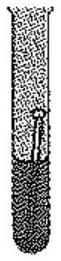
\includegraphics[width=\textwidth]{2025_10_23_74efce88ce3a451fd6b0g-072}
\captionsetup{labelformat=empty}
\caption{Không khí\\
a) và nước}
\end{center}
\end{figure}

\begin{figure}[h]
\begin{center}
  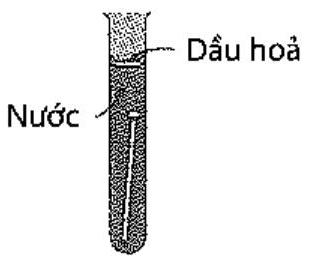
\includegraphics[width=\textwidth]{2025_10_23_74efce88ce3a451fd6b0g-072(1)}
\captionsetup{labelformat=empty}
\caption{Nước, không\\
có không khí}
\end{center}
\end{figure}

\begin{figure}[h]
\begin{center}
  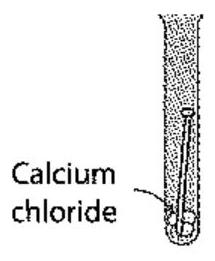
\includegraphics[width=\textwidth]{2025_10_23_74efce88ce3a451fd6b0g-072(2)}
\captionsetup{labelformat=empty}
\caption{Không khí khô,\\
c) không có nước}
\end{center}
\end{figure}

A. chỉ có ống nghiệm a).\\
B. chỉ có ống nghiệm b).\\
C. ống nghiệm\\
a) và c ).\\
D. ống nghiệm\\
b) và c).\\
22.11. Cho các trường hợp sau: (1) Bọc đinh sắt bằng dây đồng; (2) Bọc đinh sắt bằng dây kẽm; (3) Nhúng đinh sắt vào dung dịch acid.\\
Trường hợp đinh sắt bị rỉ nhanh hơn là\\
A. (1) và (2).\\
B. (1) và (3).\\
C. (2) và (3).\\
D. (1), (2) và (3).\\
22.12. Lần lượt nối thanh Zn với mỗi kim loại sau đây và cho vào dung dịch HCl . Quá trình ăn mòn thanh Zn xảy ra nhanh nhất khi nối với\\
A. Mg.\\
B. Pb.\\
C. Ag.\\
D. Cu .\\
22.13. Cho một thanh Fe tiếp xúc với một thanh Cu , sau đó nhúng vào dung dịch HCl , hiện tượng sẽ quan sát được là\\
A. thanh Fe tan và bọt khí chỉ thoát ra từ thanh Cu .\\
B. cả 2 thanh tan đồng thời và khí thoát ra từ 2 thanh.\\
C. thanh Fe tan trước và bọt khí thoát ra trên thanh Fe .\\
D. thanh Fe tan và bọt khí thoát ra từ cả thanh Fe và thanh Cu .\\
22.14. Cho các cặp kim loại nguyên chất tiếp xúc trực tiếp với nhau: Fe và $\mathrm{Pb} ; \mathrm{Fe}$ và $\mathrm{Zn} ; \mathrm{Fe}$ và $\mathrm{Sn} ; \mathrm{Fe}$ và Ni . Khi nhúng các cặp kim loại trên vào dung dịch acid, số cặp kim loại trong đó Fe bị phá huỷ trước là\\
A. 1 .\\
B. 3 .\\
C. 2 .\\
D. 4 .\\
22.15. Cho một số phương pháp bảo vệ kim loại khỏi bị ăn mòn:\\
(1) Cách li kim loại với môi trường xung quanh.\\
(2) Dùng hợp kim chống gỉ.\\
(3) Dùng chất kìm hãm.\\
(4) Ngâm kim loại trong $\mathrm{H}_{2} \mathrm{O}$.\\
(5) Dùng phương pháp điện hoá.

Các phương pháp đúng là\\
A. (1), (3), (4), (5).\\
B. (1), (2), (3), (4).\\
C. (2), (3), (4), (5).\\
D. (1), (2), (3), (5).

\section*{VAN DUNG}
22.16. Khi $100,0 \mathrm{~kg}$ sắt lên gỉ sắt hoàn toàn thì tạo thành bao nhiêu kg gỉ sắt? (Giả thiết công thức hoá học của gi sắt là $\mathrm{Fe}_{2} \mathrm{O}_{3} \cdot 3 \mathrm{H}_{2} \mathrm{O}$.) (Làm tròn kết quả đến phần nguyên).\\
Hãy chọn đúng hoăc sai cho mỗi ý a, b, c, d ở các câu 22.17-22.18.\\
22.17. Sự ăn mòn điện hoá xảy ra khi\\
a) cho miếng hợp kim $\mathrm{Ag}-\mathrm{Cu}$ trong dung dịch HCl loãng.\\
b) đặt hợp kim $\mathrm{Zn}-\mathrm{Cu}$ trong không khí ẩm.\\
c) đốt hợp kim $\mathrm{Zn}-\mathrm{Fe}$ trong bình chứa khí $\mathrm{O}_{2}$ dư.\\
d) ngâm kim loại Cu tinh khiết trong dung dịch muối ăn.\\
22.18. Sự ăn mòn điện hoá xảy ra khi nhúng thanh Fe nguyên chất vào\\
a) dung dịch HCl ;\\
b) dung dịch $\mathrm{CuCl}_{2}$;\\
c) dung dịch $\mathrm{FeCl}_{3}$;\\
d) dung dịch HCl có lẫn $\mathrm{CuCl}_{2}$.

\section*{BÀI 23}
\section*{ÔN TÂP CHƯỚNG VI}
\section*{NHAN BIET}
23.1. Phát biểu nào sau đây về đặc điểm của nguyên tử kim loại đúng?

Trong cùng một chu kì, so với các nguyên tử nguyên tố phi kim thì\\
A. nguyên tử kim loại có điện tích hạt nhân nhỏ hơn và bán kính lớn hơn nên dễ nhường electron hoá trị hơn.\\
B. nguyên tử kim loại có điện tích hạt nhân lớn hơn và bán kính lớn hơn nên dễ nhường electron hoá trị hơn.\\
C. nguyên tử kim loại có điện tích hạt nhân nhỏ hơn và bán kính nhỏ hơn nên dễ nhường electron hoá trị hơn.\\
D. nguyên tử kim loại có điện tích hạt nhân nhỏ hơn và bán kính lớn hơn nên khó nhường electron hoá trị hơn.\\
23.2. Trong bảng tuần hoàn, các nguyên tố\\
A. khối $\mathrm{s}, \mathrm{d}, \mathrm{f}$ thường là phi kim.\\
B. khối $\mathrm{s}, \mathrm{d}, \mathrm{f}$ thường là kim loại.\\
C. khối $\mathrm{s}, \mathrm{p}$ thường là kim loại.\\
D. khối $\mathrm{s}, \mathrm{p}$ thường là phi kim.\\
23.3. Kim loại dẫn điện tốt, thường dùng làm lõi dây điện là\\
A. bạc.\\
B. vàng.\\
C. đồng.\\
D. sắt.\\
23.4. Gang là vật liệu kim loại có thành phần chính là\\
A. nhôm và magnesium.\\
B. sắt và carbon.\\
C. đồng và kẽm.\\
D. đồng và thiếc.\\
23.5. Duralumin là vật liệu kìm loại chứa nguyên tố kim loại cơ bản nào sau đây?\\
A. Nhôm.\\
B. Kẽm.\\
C. Sắt.\\
D. Nickel.\\
23.6. $\mathrm{Au}, \mathrm{Ag}$ có thể tồn tại được ở dạng đơn chất trong tự nhiên vì chúng là kim loại\\
A. hoạt động hoá học mạnh.\\
B. hoạt động hoá học trung bình.\\
C. có khối lượng riêng lớn.\\
D. rất kém hoạt động hoá học.\\
23.7. Kim loại có khả năng dẫn điện vì\\
A. chúng có cấu tạo tinh thể.\\
B. trong tinh thể kim loại, các electron liên kết yếu với hạt nhân, chuyển động tự do trong toàn bộ mạng tinh thể.\\
C. trong mạng tinh thể kim loại, các anion chuyển động tự do.\\
D. trong mạng tinh thể kim loại có các cation kim loại.\\
23.8. Phát biểu nào sau đây không đúng?

Tính dẻo của kim loại là do\\
A. kim loại ở trạng thái rắn có cấu trúc tinh thể.\\
B. sự trượt của các lớp nguyên tử trong mạng tinh thể kim loại.\\
C. các electron tự do luôn chuyển động và giữ các nguyên tử kim loại liên kết với nhau.\\
D. kim loại ở trạng thái rắn không có cấu trúc tinh thể.

\section*{THONG HIEU}
23.9. Dãy kim loại nào sau đây có phản ứng với đung dịch sulfuric acid đặc, nóng tạo thành khí sulfur dioxide?\\
A. Na, K, Au.\\
B. $\mathrm{Al}, \mathrm{Fe}, \mathrm{Cu}$.\\
C. $\mathrm{Ag}, \mathrm{Au}, \mathrm{Pt}$.\\
D. $\mathrm{Cu}, \mathrm{Ag}, \mathrm{Au}$.\\
23.10. Dãy kim loại nào sau đây không đẩy đồng ra khỏi dung dịch copper(II) sulfate?\\
A. $\mathrm{Na}, \mathrm{K}, \mathrm{Ag}$.\\
B. $\mathrm{Al}, \mathrm{Fe}, \mathrm{Mg}$.\\
C. $\mathrm{Al}, \mathrm{Zn}, \mathrm{Pb}$.\\
D. $\mathrm{Mg}, \mathrm{Zn}, \mathrm{Fe}$.\\
23.11. Trong công nghiệp, kim loại natri thường được điều chế bằng phương pháp nào sau đây?\\
A. Điện phân nóng chảy.\\
B. Điện phân dung dịch.\\
C. Nhiệt luyện.\\
D. Thuỷ luyện.\\
23.12. Ngâm các mẫu sau vào dung dịch acid rồi để ngoài không khí, mẫu nào không xảy ra ăn mòn điện hoá?\\
A. Miếng gang.\\
B. Lá đồng.\\
C. Miếng tôn.\\
D. Đinh sắt.\\
23.13. Để bảo vệ khung xe đạp khỏi bị ăn mòn có thể dùng cách nào sau đây?\\
A. Ngâm trong dung dịch acid.\\
B. Bọc dây đồng quanh khung xe.\\
C. Phủ kín bề mặt bằng lớp sơn.\\
D. Để trong không khí ẩm.

Hãy chọn đúng hoặc sai cho mỗi ý $a, b, c, d$ ở câu sau.\\
23.14. a) Đồng là kim loại dẫn điện tốt nhất nên thường được dùng làm dây dẫn điện.\\
b) Duralumin thường được dùng để chế tạo vỏ máy bay.\\
c) Nhôm thường được điều chế bằng phương pháp thuỷ luyện.\\
d) Có thể bảo vệ sắt thép khỏi bị ăn mòn bằng cách gắn thêm magnesium.

\section*{VAN DUNG}
23.15. Cho khí $\mathrm{CO}(\mathrm{dư})$ đi qua ống sứ đựng $1,0 \mathrm{~g}$ hỗn hợp X gồm $\mathrm{Al}_{2} \mathrm{O}_{3}$ và CuO tới khi phản ứng xảy ra hoàn toàn. Dẫn khí đi ra vào nước vôi trong dư, tạo thành $0,4 \mathrm{~g}$ kết tủa. Thành phần phần trăm khối lượng CuO trong X là bao nhiêu?\\
23.16. Ngâm một đủnh sắt vào 200 mL dung dịch $\mathrm{CuSO}_{4}$ có nồng độ x M . Sau khi phản ứng kết thúc, lấy đinh ra khỏi dung dịch, rửa nhẹ, làm khô thấy khối lượng đỉnh sắt tăng thêm $0,8 \mathrm{~g}$. Giá trị của x là bao nhiêu?\\
23.17. Hoà tan hỗn hợp bột kim loại gồm $8,4 \mathrm{~g}$ Fe và $6,4 \mathrm{~g} \mathrm{Cu}$ vào 350 mL dung dịch $\mathrm{AgNO}_{3} 2 \mathrm{M}$. Sau khi phản ứng xảy ra hoàn toàn thu được bao nhiêu gam chất rắn?\\
23.18. Hoà tan $23,4 \mathrm{~g}$ hỗn hợp gồm $\mathrm{Al}, \mathrm{Fe}, \mathrm{Cu}$ bằng một lượng vừa đủ dung dịch $\mathrm{H}_{2} \mathrm{SO}_{4}$, thu được 15,12 lít khí $\mathrm{SO}_{2}$ (đktc) và dung dịch chứa m gam muối. Giá trị của m là bao nhiêu?

\section*{Chưong VII}
\section*{NGUYÊN TÓ NHÓM IA VA NHÓM ITA}
\section*{BÀI 24}
\section*{NGUYÊN TỐ NHÓM IA}
\section*{NHAN BIÉT}
24.1. Ở trạng thái cơ bản, nguyên tử K có cấu hình electron là $[\mathrm{Ar}] 4 \mathrm{~s}^{1}$. Trong bảng tuần hoàn, nguyên tố K thuộc nhóm\\
A. IIIA.\\
B. IA.\\
C. IVA.\\
D. IIA.\\
24.2. Khi tham gia phản ứng hoá học, mỗi nguyên tử kim loại nhóm IA đều thể hiện khuynh hướng\\
A. nhường 2 electron.\\
B. nhận 2 electron.\\
C. nhận 1 electron.\\
D. nhường 1 electron.\\
24.3. Ở điều kiện thường, các tinh thể kim loại nhóm IA đều có kiểu cấu trúc\\
A. lập phương tâm khối.\\
B. lập phương tâm mặt.\\
C. lục phương.\\
D. lập phương đơn giản.\\
24.4. Nhiệt độ nóng chảy của các kim loại nhóm IA từ Li đến Cs biến đổi như thế nào?\\
A. Tăng dần.\\
B. Không đồi.\\
C. Không có quy luật.\\
D. Giảm dần.\\
24.5. Ở điều kiện thường, kim loại có khối lượng riêng nhỏ nhất là\\
A. K.\\
B. Rb.\\
C. Li.\\
D. Na.\\
24.6. Hợp kim nào sau đây có nhiệt độ nóng chảy thấp $\left(\sim 70^{\circ} \mathrm{C}\right)$, dễ hoá lỏng nên được dùng làm chất dẫn nhiệt trong một số lò phản ứng hạt nhân?\\
A. $\mathrm{Fe}-\mathrm{C}$.\\
B. $\mathrm{Na}-\mathrm{K}$.\\
C. $\mathrm{Al}-\mathrm{Mg}$.\\
D. $\mathrm{Au}-\mathrm{Ag}$.\\
24.7. Nhận định nào sau đây về các kim loại nhóm IA không đúng?\\
A. Độ cứng thấp.\\
B. Dễ nóng chảy.\\
C. Khối lượng riêng lớn.\\
D. Dẫn điện tốt.\\
24.8. Ở một số quốc gia, khoáng vật trona là nguyên liệu chính để sản xuất soda. Thành phần hoá học chính của trona là\\
A. $3 \mathrm{NaF} \cdot \mathrm{AlF}_{3}$.\\
B. $\mathrm{NaCl} \cdot \mathrm{KCl}$.\\
C. $\mathrm{Na}_{2} \mathrm{CO}_{3} \cdot \mathrm{NaHCO}_{3} \cdot 2 \mathrm{H}_{2} \mathrm{O}$.\\
D. $\mathrm{NaNO}_{3}$.\\
24.9. Tính khử của các kim loại nhóm IA từ Li đến Cs biến đổi như thế nào?\\
A. Tăng dần.\\
B. Không đồr.\\
C. Không có quy luật.\\
D. Giảm dần.\\
24.10. Dãy nào sau đây sắp xếp các kim loại nhóm IA theo mức độ phản ứng với nước tăng dần?\\
A. $\mathrm{K}, \mathrm{Na}, \mathrm{Li}$.\\
B. $\mathrm{Na}, \mathrm{K}, \mathrm{Li}$.\\
C. Li, Na, K.\\
D. $\mathrm{K}, \mathrm{Li}, \mathrm{Na}$.\\
24.11. Kim loại nhóm IA có tính khử mạnh nhất trong các nhóm kỉm loại. Giá trị thế điện cực chuẩn nào sau đây thuộc về một kim loại trong nhóm IA?\\
A. $-0,44 \mathrm{~V}$.\\
B. $-2,93 \mathrm{~V}$.\\
C. 0 V .\\
D. $1,52 \mathrm{~V}$.\\
24.12. Khi đốt nóng tinh thể LiCl trong ngọn lửa đèn khí không màu thì tạo ra ngọn lửa có màu\\
A. da cam.\\
B. tím nhạt.\\
C. vàng.\\
D. đỏ tía.\\
24.13. Các kim loại kiềm đều hoạt động hoá học mạnh. Vì vậy, để bảo quản lâu dài, chúng thường được ngâm trong\\
A. dầu hoả.\\
B. nước máy.\\
C. ethyl alcohol.\\
D. giấm ăn.\\
24.14. Hợp chất nào sau đây vừa tác dụng được với dung dịch HCl , vừa tác dụng được với dung dịch NaOH ?\\
A. $\mathrm{NaHCO}_{3}$.\\
B. NaCl .\\
C. $\mathrm{Ba}(\mathrm{OH})_{2}$.\\
D. $\mathrm{Na}_{2} \mathrm{CO}_{3}$.\\
24.15. Trong công nghiệp, quá trình điện phân dung dịch NaCl bão hoà (điện cực trơ, màng ngăn xốp) để sản xuất các hoá chất nào sau đây?\\
A. Na và $\mathrm{Cl}_{2}$.\\
B. $\mathrm{Na}, \mathrm{H}_{2}$ và $\mathrm{Cl}_{2}$.\\
C. $\mathrm{NaOH}, \mathrm{H}_{2}$ và $\mathrm{Cl}_{2}$.\\
D. $\mathrm{NaOH}, \mathrm{O}_{2}$ và $\mathrm{Cl}_{2}$.\\
24.16. Nhỏ vài giọt dung dịch phenolphthalein vào dung dịch $\mathrm{Na}_{2} \mathrm{CO}_{3}$ thì dung dịch chuyển sang màu\\
A. tím.\\
B. vàng.\\
C. xanh.\\
D. hồng.\\
24.17. Ở các nước ôn đới, để làm giảm nhiệt độ đóng băng của nước, lằm tuyết tan, khoáng chất được rải lên tuyết là\\
A. muối mỏ.\\
B. than đá.\\
C. đá vôi.\\
D. thạch cao.\\
24.18. Diêm tiêu kali được dùng chế tạo thuốc nổ đen (làm mìn phá đá), làm phân bón (cung cấp nguyên tố N và K cho cây trồng) có công thức hoá học là\\
A. $\mathrm{KNO}_{3}$.\\
B. $\mathrm{K}_{2} \mathrm{CO}_{3}$.\\
C. KCl .\\
D. $\mathrm{K}_{2} \mathrm{SO}_{4}$,\\
24.19. Quá trình sản xuất soda bằng phương pháp Solvay không sử dụng nguyên liệu nào sau đây?\\
A. Carbon dioxide.\\
B. Muối ăn.\\
C. Xút ăn da.\\
D. Ammonia.\\
24.20. Khi đốt cháy kim loại Na trong bình chứa khí oxygen tạo thành sản phẩm là\\
A. NaO .\\
B. $\mathrm{Na}_{2} \mathrm{O}_{2}$.\\
C. $\mathrm{Na}_{2} \mathrm{O}$.\\
D. $\mathrm{NaO}_{2}$.

\section*{THONG HIEU}
24.21. Trong dãy kim loại nhóm IA từ Li đến Cs, nhiệt độ nóng chảy giảm dần do nguyên nhân nào sau đây?\\
A. Độ bền liên kết kim loại giảm dần.\\
B. Số electron hoá trị tăng dần.\\
C. Khối lượng nguyên tử tăng dần.\\
D. Độ âm điện giảm dần.\\
24.22. Trong dãy kim loại nhóm IA từ Li đến Cs , số electron hoá trị trên một đơn vị thể tích biến đổi như thế nào?\\
A. Giảm dần.\\
B. Tăng dần.\\
C. Không đồi.\\
D. Không có quy luật.\\
24.23. Khi so sánh kim loại nhóm IA với các nguyên tố khác trong cùng chu kì, nhận định nào sau đây không đúng?\\
A. Có tính khử mạnh nhất.\\
B. Có thế điện cực chuẩn âm nhất.\\
C. Có bán kính nguyên tử lớn nhất.\\
D. Có liên kết kim loại mạnh nhất.\\
24.24. Trong quá trình điện phân dung dịch NaCl với điện cực trơ có màng ngăn xốp, phân tử hay ion nào sau đây di chuyển được từ anode sang cathode qua màng ngăn xốp?\\
A. $\mathrm{Cl}^{-}$.\\
B. $\mathrm{Na}^{+}$.\\
C. $\mathrm{OH}^{-}$.\\
D. $\mathrm{Cl}_{2}$.\\
24.25. Một gia đình pha 1 kg nước muối sinh $\mathrm{li} \mathrm{NaCl} 0,9 \%$ để làm nước súc miệng. Khối lượng muối ăn cần dùng là\\
A. 9 g .\\
B. 27 g .\\
C. 18 g .\\
D. 36 g .\\
24.26. $\mathrm{X}, \mathrm{Y}, \mathrm{Z}$ là các hợp chất vô cơ của sodium, biết rằng:\\
(a) $X+Z \longrightarrow Y+\mathrm{H}_{2} \mathrm{O}$;\\
(b) $\mathrm{X} \xrightarrow{\mathrm{t}^{\circ}} \mathrm{Y}+\mathrm{CO}_{2}+\mathrm{H}_{2} \mathrm{O}$.

Các hợp chất $\mathrm{X}, \mathrm{Z}$ lần lượt là\\
A. $\mathrm{Na}_{2} \mathrm{CO}_{3}, \mathrm{NaHCO}_{3}$.\\
B. $\mathrm{NaHCO}_{3}, \mathrm{NaOH}$.\\
C. $\mathrm{NaOH}, \mathrm{Na}_{2} \mathrm{CO}_{3}$.\\
D. $\mathrm{NaHCO}_{3}, \mathrm{Na}_{2} \mathrm{CO}_{3}$.\\
24.27. Xét phản ứng nhiệt phân $\mathrm{NaHCO}_{3}$ thành $\mathrm{Na}_{2} \mathrm{CO}_{3}$ trong quá trình Solvay: $2 \mathrm{NaHCO}_{3}(\mathrm{~s}) \longrightarrow \mathrm{Na}_{2} \mathrm{CO}_{3}(\mathrm{~s})+\mathrm{CO}_{2}(\mathrm{~g})+\mathrm{H}_{2} \mathrm{O}(\mathrm{g}) \quad \Delta \mathrm{H}^{\circ}=+135,6 \mathrm{~kJ}$ Nhiệt lượng cần cung cấp để nhiệt phân 1 kg NaHCO i theo phản ứng trên là\\
A. $807,1 \mathrm{~kJ}$.\\
B. $1614,3 \mathrm{~kJ}$.\\
C. $1210,7 \mathrm{~kJ}$.\\
D. $403,6 \mathrm{~kJ}$.\\
24.28. Trong một giai đoạn của quá trình Solvay có tồn tại cân bằng giữa các muối trong dung dịch:

$$
\mathrm{NaCl}+\mathrm{NH}_{4} \mathrm{HCO}_{3} \rightleftharpoons \mathrm{NaHCO}_{3}+\mathrm{NH}_{4} \mathrm{Cl}
$$

Dựa trên tính chất nào của $\mathrm{NaHCO}_{3}$ để kết tinh muối này từ dung dịch hỗn hợp?\\
A. Độ tan thấp.\\
B. Tính lưỡng tính.\\
C. Độ bền nhiệt thấp.\\
D. Tính acid Bronsted.\\
24.29. Đun nóng tinh thể muối halide nào sau đây với dung dịch sulfuric acid đặc sẽ xảy ra phản ứng oxi hoá - khử?\\
A. NaCl .\\
B. NaF .\\
C. KCl .\\
D. KBr .\\
24.30. Dãy nào sau đây sắp xếp các dung dịch (có cùng nồng độ $0,1 \mathrm{M}$ ) theo thứ tự pH tăng dần?\\
A. $\mathrm{LiOH}, \mathrm{Na}_{2} \mathrm{CO}_{3}, \mathrm{KCl}$.\\
B. $\mathrm{Na}_{2} \mathrm{CO}_{3}, \mathrm{KCl}, \mathrm{LiOH}$.\\
C. $\mathrm{KCl}, \mathrm{Na}_{2} \mathrm{CO}_{3}, \mathrm{LiOH}$.\\
D. $\mathrm{Na}_{2} \mathrm{CO}_{3}, \mathrm{LiOH}, \mathrm{KCl}$.

Hãy chọn đúng hoặc sai cho mỗi ý a, b, c, d ở các câu 24.31-24.32.\\
24.31. Phương pháp Solvay để sản xuất $\mathrm{Na}_{2} \mathrm{CO}_{3}$ trong công nghiệp được minh hoạ ở sơ đồ sau:\\
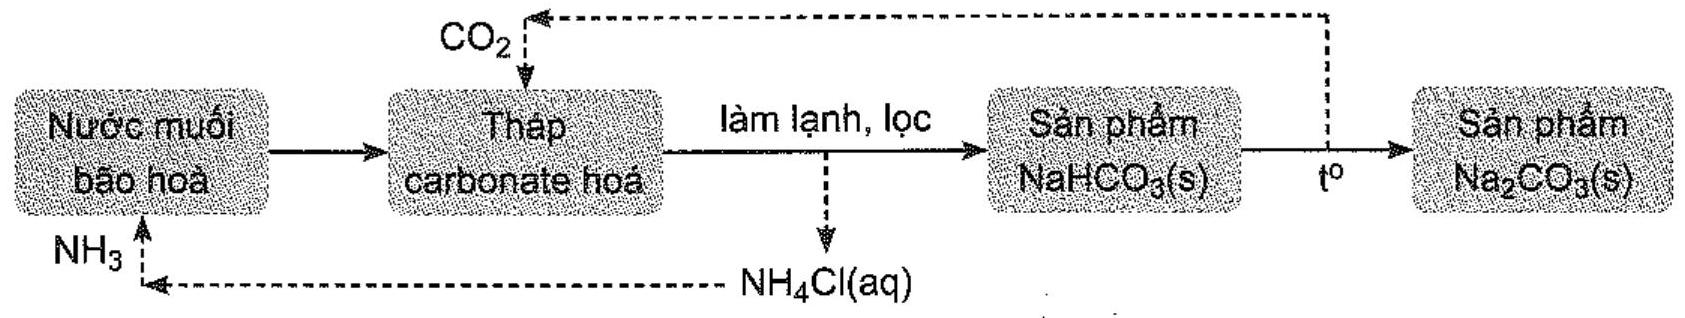
\includegraphics[max width=\textwidth, center]{2025_10_23_74efce88ce3a451fd6b0g-080}\\
a) Ion hydrogencarbonate được tạo thành tại tháp carbonate hoá.\\
b) Ở giai đoạn làm lạnh, $\mathrm{NaHCO}_{3}$ được tách biệt bằng phương pháp kết tủa.\\
c) Phản ứng chuyển hoá $\mathrm{NaHCO}_{3}$ thành $\mathrm{Na}_{2} \mathrm{CO}_{3}$ là phản ứng toả nhiệt.\\
d) Ammonia và carbon dioxide được sử dụng quay vòng trong quá trình sản xuất.\\
24.32. Quặng sylvinite là một khoáng chất phổ biến có thành phần chính là $\mathrm{NaCl} \cdot \mathrm{KCl}$. Sự phụ thuộc của độ tan các muối vào nhiệt độ được biểu diễn ở đồ thị sau.\\
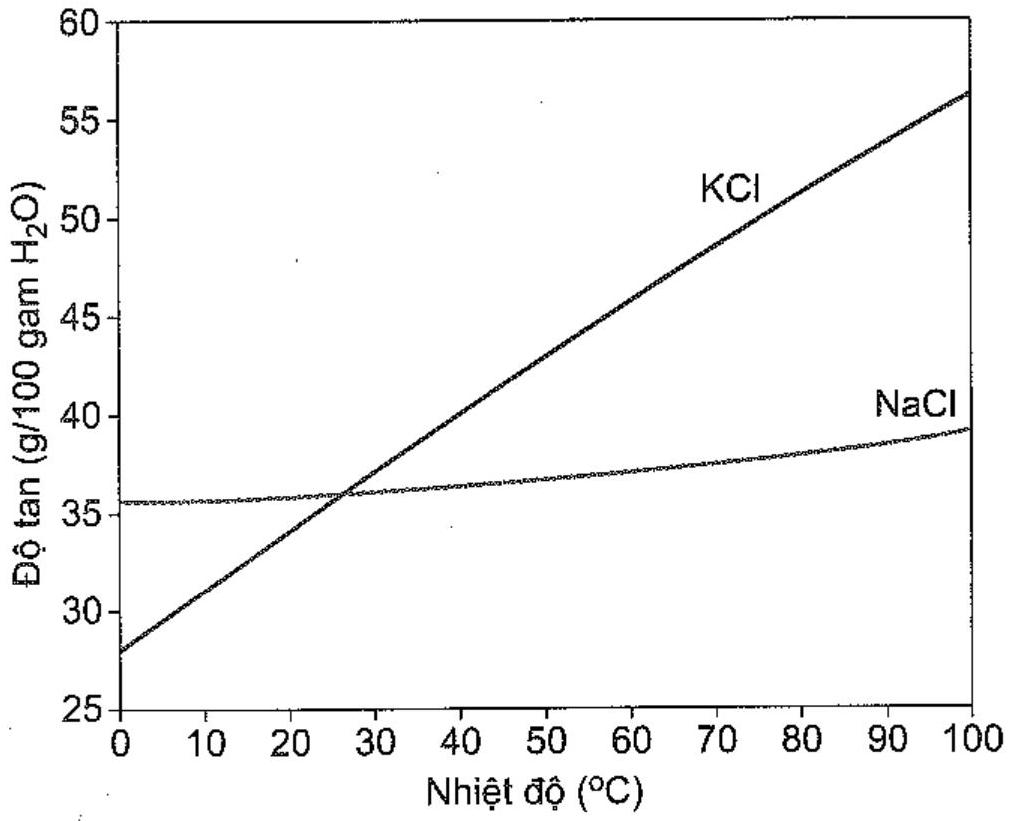
\includegraphics[max width=\textwidth, center]{2025_10_23_74efce88ce3a451fd6b0g-081}\\
a) Độ tan của KCl giảm chậm khi giảm nhiệt độ từ $100^{\circ} \mathrm{C}$ về $0^{\circ} \mathrm{C}$.\\
b) Tách được KCl khỏi dung dịch với NaCl bằng phương pháp kết tinh.\\
c) Độ tan của NaCl tăng nhanh khi tăng nhiệt độ từ $0^{\circ} \mathrm{C}$ đến $100^{\circ} \mathrm{C}$.\\
d) Độ tan của KCl giảm nhanh hơn của NaCl khi giảm nhiệt độ từ $100^{\circ} \mathrm{C}$ về $0^{\circ} \mathrm{C}$.\\
24.33. Ở $20^{\circ} \mathrm{C}$, độ tan của NaCl trong nước là $35,9 \mathrm{~g}$ trong 100 g nước. Ở nhiệt độ này, dung dịch NaCl bão hoà có nồng độ $\mathrm{a} \%$.\\
Giá trị của a là bao nhiêu? (Làm tròn kết quả đến phần mười).\\
24.34. Trong tinh thể NaCl , các ion trái dấu tiếp xúc và sắp xếp xen kẽ nhau như mô hình sau đây.

\begin{figure}[h]
\begin{center}
  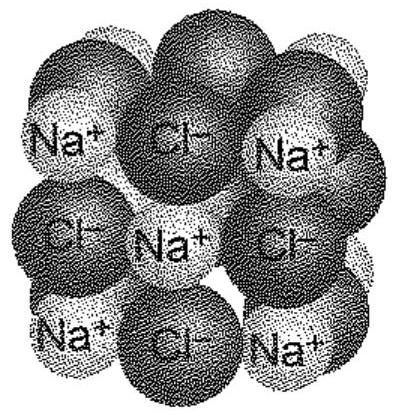
\includegraphics[width=\textwidth]{2025_10_23_74efce88ce3a451fd6b0g-081(1)}
\captionsetup{labelformat=empty}
\caption{Mô hình đặc}
\end{center}
\end{figure}

\begin{figure}[h]
\begin{center}
  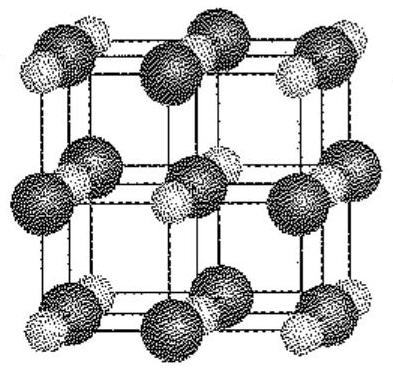
\includegraphics[width=\textwidth]{2025_10_23_74efce88ce3a451fd6b0g-081(2)}
\captionsetup{labelformat=empty}
\caption{Mô hình rỗng}
\end{center}
\end{figure}

Biết chiều dài cạnh của hình lập phương ở mô hình rỗng là $\mathrm{a}=564 \mathrm{pm}$ và bán kính ion $\mathrm{Cl}^{-}$là 182 pm .\\
Bán kính ion $\mathrm{Na}^{+}$là bao nhiêu pm ? (Làm tròn kết quả đến phần nguyên).\\
24.35. Tại một nhà máy, quặng bauxite được đun nóng với dung dịch $\mathrm{NaOH} 20 \%$ ở nhiệt độ $170^{\circ} \mathrm{C}-180^{\circ} \mathrm{C}$ để chuyển hoá $\mathrm{Al}_{2} \mathrm{O}_{3}$ thành muối dễ tan theo phương trình hoá học:

$$
\mathrm{Al}_{2} \mathrm{O}_{3}+2 \mathrm{NaOH} \xrightarrow{\mathrm{t}^{\circ}} 2 \mathrm{NaAlO}_{2}+\mathrm{H}_{2} \mathrm{O}
$$

Để hoà tan 1 tấn $\mathrm{Al}_{2} \mathrm{O}_{3}$ trong quặng bauxite cần dùng ít nhất bao nhiêu tấn dung dịch $\mathrm{NaOH} 20 \%$ ? (Làm tròn kết quả đến phần trăm).

\section*{VAN DUNG}
24.36. Cho $1,9 \mathrm{~g}$ hỗn hợp gồm muối carbonate và hydrocarbonate của một kim loại kiềm tác dụng với dung dịch HCl dư thu được 0,496 lít khí (ở đkc). Kim loại kiềm là\\
A. K\\
B. Li\\
C. Na\\
D. Rb.\\
24.37. Hoà tan hoàn toàn hỗn hợp K và Na vào nước, thu được dung dịch X và a mol khí $\mathrm{H}_{2}$. Trung hoà X cần 200 mL dung dịch $\mathrm{H}_{2} \mathrm{SO}_{4} 0,1 \mathrm{M}$. Giá trị của a là\\
A. 0,04 .\\
B. 0,02 .\\
C. 0,005 .\\
D. 0,01 .\\
24.38. Độ hoà tan của $\mathrm{NaHCO}_{3}$ ở $20^{\circ} \mathrm{C}$ và $60^{\circ} \mathrm{C}$ lần lượt là 9,6 và $16,5 \mathrm{~g} / 100 \mathrm{~g} \mathrm{H}_{2} \mathrm{O}$. Để 1 tấn dung dịch $\mathrm{NaHCO}_{3}$ bão hoà ở $60^{\circ} \mathrm{C}$ làm nguội về $20^{\circ} \mathrm{C}$ (giả thiết không có sự bay hơi nước), thu được dung dịch X và a kg chất rắn khan. Giá trị của a là\\
A. 59,23 .\\
B. 69,00 .\\
C. 54,04 .\\
D. 96,00 .

Hãy chọn đúng hoặc sai cho mỗi ý $\mathrm{a}, \mathrm{b}, \mathrm{c}, \mathrm{d}$ ở các câu 24.39-24.40.\\
24.39. a) Thứ tự tính khử giảm dần của các kim loại kiềm là: $\mathrm{Cs}, \mathrm{Rb}, \mathrm{K}, \mathrm{Na}, \mathrm{Li}$.\\
b) Phương pháp chung để điều chế kim loại kiềm là điện phân dung dịch.\\
c) Để bảo quản kim loại Na cần ngâm Na trong cồn tinh khiết.\\
d) $\mathrm{Na}_{2} \mathrm{O}$ tan trong nước tạo dung dịch trong suốt và thoát ra khí $\mathrm{H}_{2}$.\\
24.40. a) Điện phân dung dịch NaCl có màng ngăn xốp thu được $\mathrm{NaOH}, \mathrm{H}_{2}$ và $\mathrm{O}_{2}$.\\
b) $\mathrm{NaHCO}_{3}$ là hợp chất lưỡng tính.\\
c) $\mathrm{Na}_{2} \mathrm{CO}_{3}$ là nguyên liệu sản xuất thuỷ tinh.\\
d) Phương pháp Solvay sản xuất $\mathrm{NaHCO}_{3}$ từ các nguyên liệu là $\mathrm{NH}_{3}, \mathrm{NaCl}$ và $\mathrm{CO}_{2}$.\\
24.41. Nhỏ từ từ từng giọt đến hết 150 mL dung dịch HCl 1 M vào 100 mL dung dịch gồm $\mathrm{Na}_{2} \mathrm{CO}_{3} 0,5 \mathrm{M}$ và $\mathrm{NaHCO}_{3} 1 \mathrm{M}$. Sau phản ứng thu được số mol $\mathrm{CO}_{2}$ là bao nhiêu?\\
24.42. Hấp thụ hoàn toàn 2,479 lít $\mathrm{CO}_{2}$ (đkc) vào 100 mL dung dịch gồm $\mathrm{K}_{2} \mathrm{CO}_{3} 0,2 \mathrm{M}$ và KOH nồng độ $\mathrm{C} \mathrm{mol} / \mathrm{L}$, sau khi các phản ứng xảy ra hoàn toàn thu được dung dịch Y . Cho toàn bộ Y tác dụng với dung dịch $\mathrm{BaCl}_{2}$ dư, thu được $11,82 \mathrm{~g}$ kết tủa. Giá trị của C là bao nhiêu?

\section*{BÀI 25 NGUYÊN TỐ NHÓM IIA}
\section*{NHAN BIÉT}
25.1. Ở trạng thái cơ bản, cấu hình electron lớp ngoài cùng của các kim loại nhóm IIA có dạng chung là\\
A. $\mathrm{ns}{ }^{1}$.\\
B. $\mathrm{ns}^{2}$.\\
C. $n s^{2} n p^{3}$.\\
D. $n s^{2} n p^{5}$.\\
25.2. Nguyên tố calcium đóng vai trò thiết yếu cho việc phát triển xương, góp phần duy trì hoạt động của cơ bắp, truyền dẫn thần kinh, tăng cường khả năng miễn dịch. Trong cơ thể người, phần lớn calcium tập trung ở\\
A. xương.\\
B. răng.\\
C. co.\\
D. móng.\\
25.3. Trong cơ thể người, ion $\mathrm{Mg}^{2+}(\mathrm{Z}=12)$ tham gia cấu trúc tế bào, tổng hợp protein và tổng hợp chất sinh năng lượng ATP. Tổng số hạt proton và electron của ion $\mathrm{Mg}^{2+}$ là\\
A. 26 .\\
B. 24 .\\
C. 22 .\\
D. 12 .\\
25.4. Vôi đen (quặng dolomite nghiền nhỏ) được sử dụng chủ yếu trong luyện kim, phân bón và nuôi trồng thuỷ sản. Thành phần chính của vôi đen là\\
A. $3 \mathrm{Ca}_{3}\left(\mathrm{PO}_{4}\right)_{2} \cdot \mathrm{CaF}_{2}$.\\
B. $\mathrm{CaSO}_{4} \cdot 2 \mathrm{H}_{2} \mathrm{O}$.\\
C. $\mathrm{CaCO}_{3} \cdot \mathrm{MgCO}_{3}$.\\
D. CaO .\\
25.5. Ở nơi tồn ứ rác thải, chất nào sau đây được các công nhân vệ sinh môi trường dùng để xử lí tạm thời nhằm sát trùng, diệt khuẩn, phòng chống dịch bệnh?\\
A. Cát vàng.\\
B. Than đá.\\
C. Đá vôi.\\
D. Vôi bột.\\
25.6. Khi đun nóng đến $160^{\circ} \mathrm{C}$, thạch cao sống mất một phần nước trở thành thạch cao nung, được dùng để đúc khuôn trong điêu khắc, bó bột trong y học. Thành phần hoá học của thạch cao nung là\\
A. $\mathrm{CaSO}_{4} \cdot 0,5 \mathrm{H}_{2} \mathrm{O}$.\\
B. $\mathrm{Ca}\left(\mathrm{H}_{2} \mathrm{PO}_{4}\right)_{2}$.\\
C. $\mathrm{CaCO}_{3}$.\\
D. $\mathrm{Ca}(\mathrm{OH})_{2}$.\\
25.7. Trong tự nhiên, calcium sulfate tồn tại dưới dạng muối ngậm nước ( $\mathrm{CaSO}_{4} \cdot 2 \mathrm{H}_{2} \mathrm{O}$ ) được gọi là\\
A. vôi sống.\\
B. thạch cao sống.\\
C. vôi tôi.\\
D. đá vôi.\\
25.8. Hợp chất nào của calcium là thành phần hoá học chính của quặng apatite và phosphorite, được dùng trong công nghiệp sản xuất phân bón superphosphate?\\
A. $\mathrm{CaCO}_{3}$.\\
B. $\mathrm{Ca}_{3}\left(\mathrm{PO}_{4}\right)_{2}$.\\
C. $\mathrm{Ca}_{3} \mathrm{P}_{2}$.\\
D. $\mathrm{Ca}(\mathrm{OH})_{2}$.\\
25.9. Trong nông nghiệp, trộn urea hoặc phân đạm ammonium với chất nào sau đây thì sẽ làm giảm đáng kể tác dụng của phân đạm?\\
A. $\mathrm{KNO}_{3}$.\\
B. $\mathrm{Ca}\left(\mathrm{H}_{2} \mathrm{PO}_{4}\right)_{2}$.\\
C. $\mathrm{Ca}(\mathrm{OH})_{2}$.\\
D. KCl .\\
25.10. Hiện tượng "nước chảy đá mòn" và hiện tượng "xâm thực" của nước mưa vào các phiến đá vôi là do trong nước có hoà tan khí nào sau đây?\\
A. $\mathrm{O}_{2}$.\\
B. $\mathrm{N}_{2}$.\\
C. $\mathrm{CO}_{2}$.\\
D. $\mathrm{CH}_{4}$.\\
25.11. Kim loại nào sau đây cháy trong khí oxygen tạo thành sản phẩm là peroxide?\\
A. Be.\\
B. Mg .\\
C. Ca .\\
D. Ba.\\
25.12. Ở nhiệt độ thường, kim loại nào sau đây phản ứng chậm với nước?\\
A. Mg.\\
B. Ca .\\
C. Sr.\\
D. Ba.\\
25.13. Có thể nhận biết dung dịch $\mathrm{BaCl}_{2}$ bằng dung dịch chất nào sau đây?\\
A. NaOH .\\
B. $\mathrm{Na}_{2} \mathrm{CO}_{3}$.\\
C. NaCl .\\
D. $\mathrm{NaNO}_{3}$.\\
25.14. Muối nào sau đây chỉ tồn tại trong dung dịch và bị phân huỷ khi đun nóng?\\
A. $\mathrm{Ca}\left(\mathrm{NO}_{3}\right)_{2}$.\\
B. $\mathrm{CaSO}_{4}$.\\
C. $\mathrm{CaCl}_{2}$.\\
D. $\mathrm{Ca}\left(\mathrm{HCO}_{3}\right)_{2}$.\\
25.15. Nước cứng gây nhiều tác hại trong đời sống và sản xuất như đóng cặn đường ống dẫn nước, làm cho xà phòng có ít bọt khi giặt quần áo, làm giảm mùi vị thực phẩm khi nấu ăn. Nước cứng là nước có chứa nhiều các ion\\
A. $\mathrm{Mg}^{2+}$ và $\mathrm{Ca}^{2+}$.\\
B. $\mathrm{Na}^{+}$và $\mathrm{K}^{+}$.\\
C. $\mathrm{F}^{-}$và $\mathrm{Cl}^{-}$.\\
D. $\mathrm{SO}_{4}^{2-}$ và $\mathrm{CO}_{3}^{2-}$.\\
25.16. Phản ứng nào sau đây được gọi là phản ứng tôi vôi?\\
A. $\mathrm{CaCO}_{3} \xrightarrow{\mathrm{t}^{\circ}} \mathrm{CaO}+\mathrm{CO}_{2}$.\\
B. $2 \mathrm{Ca}+\mathrm{O}_{2} \longrightarrow 2 \mathrm{CaO}$.\\
C. $\mathrm{Ca}+2 \mathrm{H}_{2} \mathrm{O} \longrightarrow \mathrm{Ca}(\mathrm{OH})_{2}+\mathrm{H}_{2}$.\\
D. $\mathrm{CaO}+\mathrm{H}_{2} \mathrm{O} \longrightarrow \mathrm{Ca}(\mathrm{OH})_{2}$.\\
25.17. Khi đốt nóng tinh thể $\mathrm{BaCl}_{2}$ trong ngọn lửa đèn khí không màu thì tạo ra ngọn lửa có màu\\
A. tím nhạt.\\
B. đỏ son.\\
C. đỏ cam.\\
D. lục vàng.\\
25.18. Trong công nghiệp, kim loại kiềm thổ thường được điều chế bằng phương pháp điện phân nóng chảy muối chloride. Quá trình khử xảy ra tại cathode là\\
A. $\mathrm{M} \rightarrow \mathrm{M}^{+}+1 \mathrm{e}$.\\
B. $\mathrm{M}^{+}+1 \mathrm{e} \rightarrow \mathrm{M}$.\\
C. $\mathrm{M}^{2+}+2 \mathrm{e} \rightarrow \mathrm{M}$.\\
D. $\mathrm{M} \rightarrow \mathrm{M}^{2+}+2 \mathrm{e}$.\\
25.19. Nhận định nào sau đây về nước cứng tạm thời không đúng?\\
A. Chứa nhiều ion $\mathrm{Mg}^{2+}, \mathrm{Ca}^{2+}$.\\
B. Chứa nhiều ion ü $\overline{3}$.\\
C. Chứa nhiều ion $\mathrm{Cl}^{-}, \mathrm{SO}_{4}^{2-}$.\\
D. Đun sôi trở thành nước mềm.

\section*{THONG HIEU}
25.20. Độ tan trong dãy muối sulfate từ $\mathrm{MgSO}_{4}$ đến $\mathrm{BaSO}_{4}$ biến đổi như thế nào?\\
A. Tăng dần.\\
B. Giảm dần.\\
C. Không có quy luật.\\
D. Không đổi.\\
25.21. Độ bền nhiệt trong dãy muối carbonate từ $\mathrm{MgCO}_{3}$ đến $\mathrm{BaCO}_{3}$ biến đổi như thế nào?\\
A. Tăng dần.\\
B. Giảm dần.\\
C. Không có quy luật.\\
D. Không đổi.\\
25.22. Ở nhiệt độ phòng, hydroxide nào sau đây có độ tan lớn nhất?\\
A. $\mathrm{Mg}(\mathrm{OH})_{2}$.\\
B. $\mathrm{Sr}(\mathrm{OH})_{2}$.\\
C. $\mathrm{Ba}(\mathrm{OH})_{2}$.\\
D. $\mathrm{Ca}(\mathrm{OH})_{2}$.\\
25.23. Khi để vôi sống trong không khí ẩm một thời gian sẽ có hiện tượng một phần bị chuyển hoá trở lại thành đá vôi. Khí nào sau đây có trong không khí gây ra hiện tượng trên?\\
A. Oxygen.\\
B. Methane.\\
C. Nitrogen.\\
D. Carbon dioxide.\\
25.24. Đun nóng tinh thể $\mathrm{CaF}_{2}$ với dung dịch $\mathrm{H}_{2} \mathrm{SO}_{4}$ đặc ở nhiệt độ khoảng $250^{\circ} \mathrm{C}$, thu được khí nào sau đây?\\
A. $\mathrm{SO}_{2}$.\\
B. $F_{2}$.\\
C. HF.\\
D. $\mathrm{H}_{2} \mathrm{~S}$.\\
25.25. Cho dung dịch HCl vào dung dịch X thấy sủi bọt khí, nếu cho dung dịch $\mathrm{Ca}(\mathrm{OH})_{2}$ vào dung dịch X sinh ra kết tủa. Dung dịch X là\\
A. $\mathrm{Na}_{2} \mathrm{SO}_{4}$.\\
B. $\mathrm{KNO}_{3}$.\\
C. $\mathrm{Ca}\left(\mathrm{HCO}_{3}\right)_{2}$.\\
D. $\mathrm{BaCl}_{2}$.\\
25.26. Cho một mẩu Na vào dung dịch $\mathrm{MgSO}_{4}$ dư, thu được kết tủa X và chất khí Y . Hai chất $\mathrm{X}, \mathrm{Y}$ lần lượt là\\
A. $\mathrm{Mg}, \mathrm{O}_{2}$.\\
B. $\mathrm{Mg}, \mathrm{H}_{2}$.\\
C. $\mathrm{Mg}(\mathrm{OH})_{2}, \mathrm{H}_{2}$.\\
D. $\mathrm{Mg}(\mathrm{OH})_{2}, \mathrm{O}_{2}$.\\
25.27. Tiến hành các thí nghiệm sau:\\
(1) Cho mẩu nhỏ Na vào cốc đựng nước dư.\\
(2) Điện phân dung dịch KCl bão hoà, có màng ngăn điện cực.\\
(3) Cho dung dịch $\mathrm{H}_{2} \mathrm{SO}_{4}$ vào dung dịch $\mathrm{Ba}\left(\mathrm{HCO}_{3}\right)_{2}$.\\
(4) Đun sôi dung dịch gồm $\mathrm{CaCl}_{2}$ và $\mathrm{NaHCO}_{3}$.

Số thí nghiệm tạo ra chất khí là\\
A. 4 .\\
B. 2 .\\
C. 3 .\\
D. 1 .\\
25.28. Tiến hành các thí nghiệm sau:\\
(1) Sục khí $\mathrm{CO}_{2}$ dư vào dung dịch $\mathrm{Ca}(\mathrm{OH})_{2}$.\\
(2) Cho dung dịch NaOH dư vào dung dịch $\mathrm{Ba}\left(\mathrm{HCO}_{3}\right)_{2}$.\\
(3) Đun sôi một mẫu nước có tính cứng tạm thời.\\
(4) Cho dung dịch $\mathrm{KHSO}_{4}$ vào dung dịch $\mathrm{Ba}(\mathrm{OH})_{2}$.

Khi kết thúc phản ứng, số thí nghiệm thu được kết tủa là\\
A. 1 .\\
B. 3 .\\
C. 2 .\\
D. 4 .\\
25.29. Vôi tôi được sử dụng trong nuôi trồng thuỷ sản để cải tạo ao, đầm trước khi bắt đầu vụ mới. Khối lượng vôi tôi để cải tạo một đầm nuôi tôm rộng $3000 \mathrm{~m}^{2}$ với hàm lượng $8 \mathrm{~kg} / 100 \mathrm{~m}^{2}$ là\\
A. 300 kg .\\
B. 80 kg .\\
C. 30 kg .\\
D. 240 kg .\\
25.30. Từ hai muối X và Y thực hiện các sơ đồ phản ứng hoá học sau:\\
(a) $\mathrm{X} \longrightarrow \mathrm{X}_{1}+\mathrm{CO}_{2}$\\
(b) $\mathrm{X}_{1}+\mathrm{H}_{2} \mathrm{O} \longrightarrow \mathrm{X}_{2}$\\
(c) $\mathrm{X}_{2}+\mathrm{Y} \longrightarrow \mathrm{X}+\mathrm{Y}_{1}+\mathrm{H}_{2} \mathrm{O}$\\
(d) $\mathrm{X}_{2}+2 \mathrm{Y} \longrightarrow \mathrm{X}+\mathrm{Y}_{2}+2 \mathrm{H}_{2} \mathrm{O}$

Hai chất $\mathrm{Y}_{1}, \mathrm{Y}_{2}$ thoả mãn sơ đồ trên lần lượt là\\
A. $\mathrm{Na}_{2} \mathrm{CO}_{3}, \mathrm{NaOH}$.\\
B. $\mathrm{NaHCO}_{3}, \mathrm{Ca}(\mathrm{OH})_{2}$.\\
C. $\mathrm{Ca}(\mathrm{OH})_{2}, \mathrm{NaHCO}_{3}$.\\
D. $\mathrm{NaOH}, \mathrm{Na}_{2} \mathrm{CO}_{3}$.\\
25.31. Thực hiện các sơ đồ phản ứng hoá học sau:

$$
\begin{aligned}
& \mathrm{X}_{1}+\mathrm{H}_{2} \mathrm{O} \xrightarrow[\mathrm{mn}]{\text { dpdd }} \mathrm{X}_{2}+\mathrm{X}_{3} \uparrow+\mathrm{H}_{2} \uparrow \\
& \mathrm{X}_{2}+\mathrm{X}_{4} \longrightarrow \mathrm{BaCO}_{3} \downarrow+\mathrm{Na}_{2} \mathrm{CO}_{3}+\mathrm{H}_{2} \mathrm{O} \\
& \mathrm{X}_{4}+\mathrm{X}_{5} \longrightarrow \mathrm{BaSO}_{4} \downarrow+\mathrm{K}_{2} \mathrm{SO}_{4}+\mathrm{CO}_{2} \uparrow+\mathrm{H}_{2} \mathrm{O}
\end{aligned}
$$

Nhận định nào sau đây đúng?\\
A. $\mathrm{X}_{2}$ là KOH .\\
B. $\mathrm{X}_{5}$ là $\mathrm{KHSO}_{4}$.\\
C. $\mathrm{X}_{4}$ là $\mathrm{NaHCO}_{3}$.\\
D. $\mathrm{X}_{1}$ là KCl .\\
25.32. Tiến hành thí nghiệm theo các bước sau:

Bước 1: Chuẩn bị hai ống nghiệm, ống (1) chứa 2 mL dung dịch $\mathrm{CaCl}_{2}$, ống (2) chứa 2 mL dung dịch $\mathrm{BaCl}_{2} 1 \mathrm{M}$.\\
Bước 2: Nhỏ đồng thời vào mỗi ống nghiệm 3 giọt dung dịch $\mathrm{CuSO}_{4} 1 \mathrm{M}$, thấy ống (1) xuất hiện kết tủa chậm hơn và it hơn so với ống (2).\\
Nhận định nào sau đây đúng khi so sánh $\mathrm{CaSO}_{4}$ với $\mathrm{BaSO}_{4}$ ?\\
A. Khó nhiệt phân hơn.\\
B. Khó thuỷ phân hơn.\\
C. Dễ kết tủa hơn.\\
D. Dễ tan hơn.\\
25.33. Một cốc nước chứa nhiều các ion sau: $\mathrm{Ca}^{2+}, \mathrm{Mg}^{2+}, \mathrm{Cl}^{-}, \mathrm{SO}_{4}^{2-}$. Nước trong cốc trên thuộc loại\\
A. có tính cứng vĩnh cửu.\\
B. không có tính cứng.\\
C. có tính cứng tạm thời.\\
D. có tính cứng toàn phần.\\
25.34. Cho các nhận định sau về tác hại của nước cứng:\\
(1) làm giảm bọt khi giặt quần áo bằng xà phòng;\\
(2) làm đường ống dẫn nước đóng cặn, giảm lưu lượng nước;\\
(3) làm thức ăn lâu chín và giảm mùi vị;\\
(4) làm nồi hơi phủ cặn, gây tốn nhiên liệu và có nguy cơ gây nổ.

Số nhận định đúng là\\
A. 2 .\\
B. 1 .\\
C. 3 .\\
D. 4 .

Hãy chọn đúng hoặc sai cho mỗi ý a, b, c, đở các câu 25.35-25.37.\\
25.35. a) Thạch cao sống có công thức $\mathrm{CaSO}_{4} \cdot 2 \mathrm{H}_{2} \mathrm{O}$.\\
b) Dùng dung dịch HCl có thể làm mềm nước cứng tạm thời.\\
c) Dùng giấm ăn đặc có thể làm sạch cặn ở đáy ấm đun nước.\\
d) Phản ứng giữa $\mathrm{NaHCO}_{3}$ và $\mathrm{Ba}(\mathrm{OH})_{2}$ tạo kết tủa và khí.

\section*{VAN DUNG}
25.36. Cho độ tan của các hydroxide kim loại nhóm IIA ở $20^{\circ} \mathrm{C}$ như sau:

\begin{center}
\begin{tabular}{|c|c|c|c|c|}
\hline
Hydroxide & $\mathrm{Mg}(\mathrm{OH})_{2}$ & $\mathrm{Ca}(\mathrm{OH})_{2}$ & $\mathrm{Sr}(\mathrm{OH})_{2}$ & $\mathrm{Ba}(\mathrm{OH})_{2}$ \\
\hline
\begin{tabular}{c}
P 0 tan \\
$(\mathrm{g} / 100 \mathrm{~g}$ nưoc $)$ \\
\end{tabular} & 0,00125 & 0,173 & 1,77 & 3,89 \\
\hline
\end{tabular}
\end{center}

(Nguồn: John A. Dean (1999), Hand book of Chemistry, Fifteenth Edition, McGraw-Hill, Inc.)\\
a) Độ tan của các hydroxide giảm dần từ $\mathrm{Mg}(\mathrm{OH})_{2}$ đến $\mathrm{Ba}(\mathrm{OH})_{2}$.\\
b) Mức độ phản ứng với nước tăng dần từ Mg đến Ba .\\
c) $\mathrm{O}^{\circ} 20^{\circ} \mathrm{C}$, nồng độ dung dịch $\mathrm{Ba}(\mathrm{OH})_{2}$ bão hoà là $3,89 \%$.\\
d) $\mathrm{Mg}(\mathrm{OH})_{2}$ là chất không tan, $\mathrm{Ca}(\mathrm{OH})_{2}$ là chất ít tan.\\
25.37. Các muối carbonate của kim loại nhóm IIA đều bị phân huỷ bởi nhiệt.

Xét phản ứng nhiệt phân:

$$
\mathrm{MCO}_{3}(\mathrm{~s}) \xrightarrow{\mathrm{t}^{\circ}} \mathrm{MO}(\mathrm{~s})+\mathrm{CO}_{2}(\mathrm{~g}) \quad \Delta_{\mathrm{r}} \mathrm{H}_{298}^{\mathrm{o}}
$$

Cho biết:

\begin{center}
\begin{tabular}{|c|c|c|c|c|}
\hline
Muói & $\mathrm{MgCO}_{3}(\mathrm{~s})$ & $\mathrm{CaCO}_{3}(\mathrm{~s})$ & $\mathrm{SrCO}_{3}(\mathrm{~s})$ & $\mathrm{BaCO}_{3}(\mathrm{~s})$ \\
\hline
$\Delta, \mathrm{H}_{298}^{\mathrm{o}}(\mathrm{kJ})$ & 100,7 & 179,2 & 234,6 & 271,5 \\
\hline
\end{tabular}
\end{center}

(Nguồn: John A. Dean (1999), Hand book of Chemistry, Fifteenth Edition, McGraw-Hill, Inc.)\\
Nhiệt độ bắt đầu xảy ra phản ứng nhiệt phân (sắp xếp ngẫu nhiên) các muối carbonate là $882^{\circ} \mathrm{C} ; 1360^{\circ} \mathrm{C} ; 542^{\circ} \mathrm{C} ; 1155^{\circ} \mathrm{C}$.\\
a) Độ bền nhiệt của các muối tăng dần từ $\mathrm{MgCO}_{3}$ đến $\mathrm{BaCO}_{3}$.\\
b) Các phản ứng nhiệt phân ở trên đều là phản ứng toả nhiệt.\\
c) Ở nhiệt độ $1155^{\circ} \mathrm{C}$, phản ứng nhiệt phân $\mathrm{SrCO}_{3}$ bắt đầu xảy ra.\\
d) Trong quá trình nung vôi xảy ra phản ứng nhiệt phân $\mathrm{CaCO}_{3}$.\\
25.38. Ở $20^{\circ} \mathrm{C}$, độ tan trong nước của $\mathrm{Ca}(\mathrm{OH})_{2}$ là $0,173 \mathrm{~g}$ trong 100 g nước. Ở nhiệt độ này, nước vôi trong bão hoà ( $\operatorname{col} \mathrm{D}=1 \mathrm{~g} / \mathrm{mL}$ ) có nồng độ mol là $\mathrm{a} \cdot 10^{-2} \mathrm{~mol} / \mathrm{L}$. Giá trị của a là bao nhiêu? (Làm tròn kết quả đến phần mười).\\
25.39. Ở nhiệt độ cao, magnesium nitrate bị phân huỷ theo phản ứng:\\
$\mathrm{Mg}\left(\mathrm{NO}_{3}\right)_{2}(\mathrm{~s}) \xrightarrow{\mathrm{t}^{\circ}} \mathrm{MgO}(\mathrm{s})+2 \mathrm{NO}_{2}(\mathrm{~g})+\frac{1}{2} \mathrm{O}_{2}(\mathrm{~g}) \quad \Delta_{\mathrm{r}} \mathrm{H}^{\circ}=?$\\
Cho biết:

\begin{center}
\begin{tabular}{|c|c|c|c|c|}
\hline
Chát & $\mathrm{Mg}\left(\mathrm{NO}_{3}\right)_{2}(\mathrm{~s})$ & $\mathrm{MgO}(\mathrm{s})$ & $\mathrm{NO}_{2}(\mathrm{~g})$ & $\mathrm{O}_{2}(\mathrm{~g})$ \\
\hline
$\Delta_{\mathrm{f}} \mathrm{H}_{298}^{\mathrm{o}}(\mathrm{kJ} / \mathrm{mol})$ & $-790,6$ & $-601,6$ & $+33,1$ & 0 \\
\hline
\end{tabular}
\end{center}

Biến thiên enthalpy chuẩn của phản ứng trên là bao nhiêu kJ? (Làm tròn kết quả đến phần nguyên).\\
25.40. Ở điều kiện thường, tinh thể Ca có $\mathrm{D}=1,55 \mathrm{~g} / \mathrm{cm}^{3}$. Giả thiết các nguyên tử Ca là những hình cầu chiếm $74 \%$ thể tích tinh thể, phần còn lại là khe rỗng. Cho biết:

\begin{itemize}
  \item Công thức tính thể tích hình cầu: $\mathrm{V}=\frac{4}{3} \cdot \pi \cdot \mathrm{r}^{3}$.
  \item Số Avogadro $\mathrm{N}_{\mathrm{A}}=6,023 \cdot 10^{23}$ và số pi $\pi=3,1416$.
\end{itemize}

Bán kính nguyên tử Ca là bao nhiêu pm? (Làm tròn kết quả đến phần nguyên).\\
25.41. Cho 200 mL dung dịch $\mathrm{Ba}(\mathrm{OH})_{2} 0,1 \mathrm{M}$ vào 300 mL dung dịch $\mathrm{NaHCO}_{3} 0,1 \mathrm{M}$, thu được dung dịch X và kết tủa Y . Cho từ từ dung dịch $\mathrm{HCl} 0,25 \mathrm{M}$ vào X đến khi bắt đầu có khí sinh ra thì hết V mL . Biết các phản ứng đều xảy ra hoàn toàn. Giá trị của V là bao nhiêu?

\section*{BÀl 26}
\section*{ÔN TẬP CHƯONG VIII}
\section*{NHAN BIÉT}
26.1. Trong nhóm IA và IIA, theo chiều từ trên xuống dưới trong mỗi nhóm, tính kim loại biến đổi như thế nào?\\
A. Không đổi.\\
B. Giảm dần.\\
C. Tăng dần.\\
D. Không có quy luật.\\
26.2. Khi đưn nóng nước tự nhiên, muối nào sau đây bị phân huỷ tạo thành cặn đá vôi trong phích nước, ấm đun nước?\\
A. $\mathrm{Ca}_{3}\left(\mathrm{PO}_{4}\right)_{2}$.\\
B. $\mathrm{CaCl}_{2}$.\\
C. $\mathrm{CaSO}_{4}$.\\
D. $\mathrm{Ca}\left(\mathrm{HCO}_{3}\right)_{2}$.\\
26.3. Trong quá trình Solvay, $\mathrm{NH}_{3}$ được tái chế khi cho dụng dịch $\mathrm{NH}_{4} \mathrm{Cl}$ tác dụng với\\
A. CaO .\\
B. NaOH .\\
C. KOH .\\
D. $\mathrm{Ba}(\mathrm{OH})_{2}$.\\
26.4. Ion $\mathrm{Ca}^{2+}(\mathrm{Z}=20)$ đóng vai trò thiết yếu trong việc phát triển xương, giúp duy trì hoạt động của cơ bắp, kích thích máu lưu thông, điều tiết một số loại hormone,... Tổng số proton và electron của ion $\mathrm{Ca}^{2+}$ là\\
A. 40 .\\
B. 42 .\\
C. 38 .\\
D. 18 .\\
26.5. Ở nhiệt độ phòng, muối nào sau đây dễ tan trong nước?\\
A. $\mathrm{SrSO}_{4}$.\\
B. $\mathrm{MgSO}_{4}$.\\
C. $\mathrm{CaSO}_{4}$.\\
D. $\mathrm{BaSO}_{4}$.\\
26.6. Khi đốt nóng tinh thể NaCl trong ngọn lửa đèn khí không màu thì tạo ra ngọn lửa có màu\\
A. đỏ cam.\\
B. tím nhạt.\\
C. vàng.\\
D. đỏ tía.\\
26.7. Các đại dương là những kho muối vô tận với nhiều khoáng chất có giá trị dinh dưỡng cao. Trong nước biển, hai nguyên tố kim loại có nhiều nhất là\\
A. sodium và magnesium.\\
B. đồng và kẽm.\\
C. nhôm và sắt.\\
D. vàng và bạc.\\
26.8. Kim loại Na ở chu kì 3, nhóm IA trong bảng tuần hoàn. Cấu hình electron lớp ngoài cùng của nguyên tử Na ở trạng thái cơ bản là\\
A. $3 \mathrm{~s}^{2} 3 \mathrm{p}^{5}$.\\
B. $3 \mathrm{~s}^{2}$.\\
C. $3 \mathrm{~s}^{1}$.\\
D. $3 s^{2} 3 p^{1}$.\\
26.9. Các hợp chất dễ tan của kim loại kiềm, kiềm thổ là thành phần cung cấp dinh dưỡng của nhiều loại phân bón hoá học phổ biến.\\
Hợp chất nào sau đây dễ tan, là thành phần dinh dưỡng chính trong phân bón superphosphate?\\
A. KCl .\\
B. $\mathrm{CaSO}_{4} \cdot 2 \mathrm{H}_{2} \mathrm{O}$.\\
C. $\mathrm{NaNO}_{3}$.\\
D. $\mathrm{Ca}\left(\mathrm{H}_{2} \mathrm{PO}_{4}\right)_{2}$.

\section*{THONG HIEU}
26.10. Kim loại nhóm IA nào sau đây dễ mất electron hoá trị nhất, được dùng sản xuất tế bào quang điện?\\
A. Cs.\\
B. Li .\\
C. Na.\\
D. K.\\
26.11. Trong các kim loại nhóm IA từ Li đến Cs, nhiệt độ nóng chảy và độ cứng biến đổi như thế nào?\\
A. Không đổi.\\
B. Giảm dần.\\
C. Tăng dần.\\
D. Không có quy luật.\\
26.12. Thực hiện bốn phản ứng hoá học theo sơ đồ:

$$
\mathrm{NaOH} \xrightarrow{+\mathrm{CO}_{2}} \mathrm{X} \xrightarrow{+\mathrm{NaOH}} \mathrm{Y} \xrightarrow{+\mathrm{Ca}(\mathrm{OH})_{2}} \mathrm{Z} \xrightarrow{\mathrm{t}^{\circ}} \mathrm{T} .
$$

Biết $\mathrm{X}, \mathrm{Y}, \mathrm{Z}, \mathrm{T}$ là các hợp chất của kim loại. Công thức hoá học của T là\\
A. NaOH .\\
B. $\mathrm{CaCO}_{3}$.\\
C. $\mathrm{Na}_{2} \mathrm{CO}_{3}$.\\
D. CaO .\\
26.13. Xét phản ứng phân huỷ muối carbonate của kim loại nhóm IIA:

$$
\mathrm{MCO}_{3}(\mathrm{~s}) \longrightarrow \mathrm{MO}(\mathrm{~s})+\mathrm{CO}_{2}(\mathrm{~g}) \quad \Delta_{\mathrm{r}} \mathrm{H}_{298}^{\mathrm{o}}
$$

Từ $\mathrm{MgCO}_{3}$ đến $\mathrm{BaCO}_{3}$, biến thiên enthalpy chuẩn của phản ứng biến đổi như thế nào?\\
A. Không đổi.\\
B. Giảm dần.\\
C. Tăng dần.\\
D. Không có quy luật.\\
26.14. Ở nhiệt thường, độ tan của các hydroxide tăng dần trong dãy từ $\mathrm{Mg}(\mathrm{OH})_{2}$ đến $\mathrm{Ba}(\mathrm{OH})_{2}$. Từ thông tin này có thể dự đoán được khả năng phản ứng với nước của các kim loại từ Mg đến Ba biến đổi như thế nào?\\
A. Tăng dần.\\
B. Không đồi.\\
C. Không có quy luật.\\
D. Giảm dần.\\
26.15. Nước chứa nhiều các ion nào sau đây có tính cứng toàn phần?\\
A. $\mathrm{Mg}^{2+}, \mathrm{Ca}^{2+}, \mathrm{HCO}_{3}^{-}, \mathrm{SO}_{4}^{2-}$.\\
B. $\mathrm{Na}^{+}, \mathrm{K}^{+}, \mathrm{SO}_{4}^{2-}, \mathrm{Cl}^{-}$.\\
C. $\mathrm{Mg}^{2+}, \mathrm{Ca}^{2+}, \mathrm{HCO}_{3}^{-}$.\\
D. $\mathrm{Mg}^{2+}, \mathrm{Ca}^{2+}, \mathrm{SO}_{4}^{2-}, \mathrm{Cl}^{-}$.\\
26.16. Phân tích một mẫu nước tự nhiên thấy chứa nhiều các ion: $\mathrm{Na}^{+}, \mathrm{Ca}^{2+}, \mathrm{HCO}_{3}^{-}$, $\mathrm{Cl}^{-}$và $\mathrm{SO}_{4}^{2-}$. Chất nào sau đây có thể làm mềm mẫu nước trên?\\
A. $\mathrm{Na}_{2} \mathrm{CO}_{3}$.\\
B. $\mathrm{Ca}(\mathrm{OH})_{2}$.\\
C. NaOH .\\
D. HCl .\\
26.17. Một loại nước cứng khi đun sôi thì trở thành nước mềm. Trong loại nước này có hoà tan những hợp chất nào sau đây?\\
A. $\mathrm{Ca}\left(\mathrm{HCO}_{3}\right)_{2}$ và $\mathrm{Mg}\left(\mathrm{HCO}_{3}\right)_{2}$.\\
B. $\mathrm{Ca}\left(\mathrm{HCO}_{3}\right)_{2}$ và $\mathrm{MgSO}_{4}$.\\
C. $\mathrm{CaSO}_{4}$ và $\mathrm{MgCl}_{2}$.\\
D. $\mathrm{MgCl}_{2}$ và $\mathrm{CaCl}_{2}$.\\
26.18. Cho sơ đồ chuyển hoá sau:

$$
\mathrm{CaO} \xrightarrow{+\mathrm{X}} \mathrm{Y} \xrightarrow{+\mathrm{Z}} \mathrm{CaCO}_{3} \xrightarrow{+\mathrm{Z}+\mathrm{X}} \mathrm{~T} \xrightarrow{+\mathrm{E}} \mathrm{CaSO}_{4} .
$$

Biết: $X, Y, Z, T, E$ là các hợp chất khác nhau; mỗi mũi tên ứng với một phương trình hoá học. Các chất $\mathrm{Z}, \mathrm{E}$ thoả mãn sơ đồ trên lần lượt là\\
A. $\mathrm{Na}_{2} \mathrm{CO}_{3}, \mathrm{H}_{2} \mathrm{SO}_{4}$. .\\
B. $\mathrm{CO}_{2}, \mathrm{KHSO}_{4}$.\\
C. $\mathrm{NaHCO}_{3}, \mathrm{Na}_{2} \mathrm{SO}_{4}$.\\
D. $\mathrm{CO}_{2}, \mathrm{BaSO}_{4}$.\\
26.19. Các dung dịch muối ăn, phèn chua, nước vôi trong được kí hiệu ngẫu nhiên là $X, Y, Z$. Một số kết quả thí nghiệm được ghi ở bảng dưới đây.

\begin{center}
\begin{tabular}{|c|l|l|}
\hline
Mâu thư & \multicolumn{1}{|c|}{Thuọc thí} & Hièn tưong \\
\hline
X & Dung dịch phenolphthalein & Chuyển màu hồng \\
\hline
Z & Dung dịch $\mathrm{BaCl}_{2}$ & Có kết tủa trắng \\
\hline
\end{tabular}
\end{center}

Các dung dịch ban đầu tương ứng với các kí hiệu là\\
A. $Y, Z, X$.\\
B. Z, X, Y.\\
C. $X, Y, Z$.\\
D. Y, X, Z.

Hãy chọn đúng hoăc sai cho mỗi ý a, b, c, d ở các câu 26.20-26.21.\\
26.20. Sodium chloride là hợp chất ion.\\
a) Ở trạng thái nóng chảy, sodium chloride có khả năng dẫn điện.\\
b) Sodium chloride có nhiệt độ nóng chảy cao.\\
c) Trong tinh thể sodium chloride, các ion có thể di chuyển tự do.\\
d) Khi dùng búa đập vào hạt muối thì hạt muối bị biến dạng do có tính dẻo.

\section*{VAN DUNG}
26.21. Cho độ tan của $\mathrm{CaSO}_{4} \cdot 2 \mathrm{H}_{2} \mathrm{O}$ trong nước ở các nhiệt độ như sau:

\begin{center}
\begin{tabular}{|c|c|c|c|c|c|c|}
\hline
Whief do ( e C ) & 0 & 10 & 20 & 40 & 60 & 80 \\
\hline
Do tan ( $\mathrm{g} / 100 \mathrm{~g}$ nuóc) & 0,223 & 0,244 & 0,255 & 0,265 & 0,244 & 0,234 \\
\hline
\end{tabular}
\end{center}

a) Độ tan của $\mathrm{CaSO}_{4} \cdot 2 \mathrm{H}_{2} \mathrm{O}$ trong nước tăng dần theo nhiệt độ từ $0^{\circ} \mathrm{C}$ đến $80^{\circ} \mathrm{C}$.\\
b) $\mathrm{O}^{\circ} 20^{\circ} \mathrm{C}$, dung dịch $\mathrm{CaSO}_{4}$ bão hoà pha chế từ $\mathrm{CaSO}_{4} \cdot 2 \mathrm{H}_{2} \mathrm{O}$ có nồng độ $0,25 \%$.\\
c) $\mathrm{CaSO}_{4} \cdot 2 \mathrm{H}_{2} \mathrm{O}$ là hợp chất dễ tan ở nhiệt độ $80^{\circ} \mathrm{C}$.\\
d) Calcium sulfate dễ tan nhất trong các muối sulfate của kim loại nhóm IIA.\\
26.22. Hấp thụ hoàn toàn $1,408 \mathrm{~g}$ khí $\mathrm{CO}_{2}$ vào 300 mL dung dịch $\mathrm{Ba}(\mathrm{OH})_{2}$ a $\mathrm{mol} / \mathrm{L}$, thu được $3,152 \mathrm{~g}$ kết tủa. Giá trị của a là bao nhiêu?\\
26.23. Một hộ gia đình mua vôi sống để khử chua cho một thửa ruộng có diện tích là $720 \mathrm{~m}^{2}$ với liều lượng $2 \mathrm{~kg} / 100 \mathrm{~m}^{2}$. Biết giá vôi sống là $20 \mathrm{nghìn} \mathrm{đồng/kg}$. Hộ gia đình trên cần bao nhiêu nghìn đồng để mua vôi sống?\\
26.24. Hấp thụ $0,06 \mathrm{~mol} \mathrm{CO}_{2}$ vào dung dịch chứa a $\mathrm{mol} \mathrm{Ba}(\mathrm{OH})_{2}$, thu được 2 b mol kết tủa. Mặt khác, nếu hấp thụ $0,08 \mathrm{~mol} \mathrm{CO}_{2}$ vào dung dịch chứa a $\mathrm{mol} \mathrm{Ba}(\mathrm{OH})_{2}$, thu được b mol kết tủa. Giá trị của a là bao nhiêu?\\
26.25. Cho m gam NaOH vào 2 lít dung dịch $\mathrm{NaHCO}_{3}$ nồng độ $\mathrm{a} \mathrm{mol} / \mathrm{L}$, thu được 2 lít dung dịch X . Lấy 1 lít dung dịch X tác dụng với dung dịch $\mathrm{BaCl}_{2}$ dư thu được $11,82 \mathrm{~g}$ kết tủa. Mặt khác, cho 1 lít dung dịch X vào dung dịch $\mathrm{CaCl}_{2}$ dư rồi đun nóng, sau khi kết thúc các phản ứng thu được $7,0 \mathrm{~g}$ kết tủa. Giá trị của m là bao nhiêu?

\section*{Chuong VIII SO LUƠC VỂDÁY KIM LOAI CHUYÊN TIẾP THÚNHÁT VÀ PHƯC CHÁT}
\section*{BÀI 27}
\section*{ĐAI CƯONG VỀ KIM LOAI CHUYỂN TIẾP DÃY THÚ NHẤT}
\section*{NHAN BIET}
27.1. Kim loại nào sau đây thuộc dãy kim loại chuyển tiếp thứ nhất?\\
A. Ti.\\
B. Al.\\
C. Ba.\\
D. Na.\\
27.2. Kim loại được mạ lên sắt để bảo vệ sắt và dùng để chế tạo thép không gỉ (dùng làm thìa, dao, dụng cụ y tế,...) là\\
A. Na.\\
B. Mg .\\
C. Cr.\\
D. Ca.\\
27.3. Nguyên tử manganese có số oxi hoá +4 trong hợp chất nào sau đây?\\
A. $\mathrm{KMnO}_{4}$.\\
B. $\mathrm{K}_{2} \mathrm{MnO}_{4}$.\\
C. $\mathrm{MnO}_{2}$.\\
D. $\mathrm{MnSO}_{4}$.\\
27.4. Trong hợp chất $\mathrm{K}_{2} \mathrm{Cr}_{2} \mathrm{O}_{7}$, số oxi hoá của nguyên tử Cr là\\
A. +6 .\\
B. +3 .\\
C. +2 .\\
D. 0 .\\
27.5. Sắt được sử dụng để sản xuất nam châm trong các máy phát điện và nhiều thiết bị điện (loa, chuông, ti vi, máy tính, điện thoại,...) dựa trên tính chất nào sau đây?\\
A. Tính dẫn điện.\\
B. Tính dẫn nhiệt.\\
C. Tính dẻo.\\
D. Tính nhiễm từ.\\
27.6. Đồng kim loại được sử dụng để chế tạo dây dẫn điện, thiết bị điện,... dựa trên tính chất vật lí đặc trưng nào sau đây?\\
A. Dẫn điện tốt.\\
B. Tính dẻo.\\
C. Dẫn nhiệt tốt.\\
D. Ánh kim.\\
27.7. Ở trạng thái cơ bản, cấu hình electron của nguyên tử nào sau đây có phân lởp 3d bão hoà?\\
A. $\mathrm{Sc}(\mathrm{Z}=21)$.\\
B. $\mathrm{Cu}(\mathrm{Z}=29)$.\\
C. Ni $(Z=28)$.\\
D. $\mathrm{Mn}(\mathrm{Z}=25)$.\\
27.8. Nguyên tố nào sau đây không thể hiện xu hướng có nhiều số oxi hoá trong hợp chất?\\
A. Cr.\\
B. Mn.\\
C. Fe.\\
D. Mg.\\
27.9. Nguyên tố kim loại có trong hemoglobin làm nhiệm vụ vận chuyển oxygen, duy trì sự sống là\\
A. sodium.\\
B. magnesium.\\
C. nhôm.\\
D. sắt.\\
27.10. Trong dãy kim loại chuyển tiếp thứ nhất, kim loại có độ cứng cao nhất là\\
A. Ti.\\
B. Fe.\\
C. Cr.\\
D. Cu .\\
27.11. Trong dãy kim loại chuyển tiếp thứ nhất, hai kim loại nào sau đây đều là kim loại nhẹ ( $\mathrm{D}<5 \mathrm{~g} / \mathrm{cm}^{3}$ )?\\
A. $\mathrm{Cr}, \mathrm{Mn}$.\\
B. $\mathrm{Fe}, \mathrm{Co}$.\\
C. Sc, Ti.\\
D. Ni, Cu.\\
27.12. Cấu hình electron của nguyên tử vanadium ở trạng thái cơ bản là $[\mathrm{Ar}] 3 \mathrm{~d}^{3} 4 \mathrm{~s}^{2}$. Trong bảng tuần hoàn, nguyên tố vanadium thuộc nhóm\\
A. VB.\\
B. IB.\\
C. VIB.\\
D. IIB.\\
27.13. Muối nào sau đây có khả năng làm mất màu thuốc tím trong môi trường sulfuric acid loãng?\\
A. $\mathrm{Na}_{2} \mathrm{SO}_{4}$.\\
B. $\mathrm{FeSO}_{4}$.\\
C. $\mathrm{MgSO}_{4}$.\\
D. $\mathrm{Fe}_{2}\left(\mathrm{SO}_{4}\right)_{3}$.\\
27.14. Từ cấu hình electron của nguyên tữ Cu ở trạng thái cơ bản là $[\mathrm{Ar}] 3 \mathrm{~d}^{10} 4 \mathrm{~s}^{1}$, xác định được cấu hình electron của ion $\mathrm{Cu}^{2+}$ là\\
A. $[\mathrm{Ar}] 3 \mathrm{~d}^{9}$.\\
B. $[\mathrm{Ar}] 3 \mathrm{~d}^{8} 4 \mathrm{~s}^{1}$.\\
C. $[\mathrm{Ar}] 3 \mathrm{~d}^{10}$.\\
D. $[\mathrm{Ar}] 3 \mathrm{~d}^{8}$.\\
27.15. Trong dãy kim loại chuyển tiếp thứ nhất, kim loại có tính dẫn điện tốt nhất là\\
A. Fe.\\
B. Ti.\\
C. Cu .\\
D. Mn.\\
27.16. Nguyên tử Cr có cấu hình electron ở trạng thái cơ bản là $[\mathrm{Ar}] 3 \mathrm{~d}^{5} 4 \mathrm{~s}^{1}$. Trong phản ứng hoá học, khi nguyên tử Cr nhường đi 3 electron để tạo thành ion $\mathrm{Cr}^{3+}$, số electron còn lại trên phân lớp 3d là\\
A. 5 .\\
B. 4 .\\
C. 3 .\\
D. 2 .\\
27.17. Nguyên tố nào sau đây được mệnh darh là "nguyên tố của màu sắc" do có khả năng thể hiện màu sắc phong phú?\\
A. Sắt.\\
B. Đồng.\\
C. Nickel.\\
D. Chromium.\\
27.18. Dung dịch nào sau đây có màu vàng chanh?\\
A. $\mathrm{CuSO}_{4}$.\\
B. $\mathrm{FeCl}_{3}$.\\
C. $\mathrm{KMnO}_{4}$.\\
D. $\mathrm{FeSO}_{4}$.\\
27.19. Dãy kim loại nào sau đây sắp xếp theo thứ tự tăng dần nhiệt độ nóng chảy?\\
A. $\mathrm{Na}, \mathrm{Fe}, \mathrm{Mg}$.\\
B. $\mathrm{Na}, \mathrm{Mg}, \mathrm{Fe}$.\\
C. $\mathrm{Fe}, \mathrm{Mg}, \mathrm{Na}$.\\
D. $\mathrm{Mg}, \mathrm{Fe}, \mathrm{Na}$.\\
27.20. Sự hình thành các nguyên tố chuyển tiếp dãy thứ nhất là do có sự sắp xếp lần lượt các electron vào phân lớp\\
A. 3d.\\
B. 4s.\\
C. 4 p .\\
D. 3 p .\\
27.21. Ion nào sau đây không có electron trên phân lớp 3d và không có màu trong dung dịch nước?\\
A. $\mathrm{Fe}^{3+}$.\\
B. $\mathrm{Cr}^{3+}$.\\
C. $\mathrm{Ti}^{3+}$.\\
D. $\mathrm{Sc}^{3+}$.\\
27.22. Oxide nào sau đây có màu trắng?\\
A. $\mathrm{Fe}_{2} \mathrm{O}_{3}$.\\
B. $\mathrm{Cr}_{2} \mathrm{O}_{3}$.\\
C. $\mathrm{Al}_{2} \mathrm{O}_{3}$.\\
D. CuO .\\
27.23. Ion nào sau đây vừa có khả năng thể hiện tính khử, vừa có khả năng thể hiện tính oxi hoá?\\
A. $\mathrm{Cr}^{3+}$.\\
B. $\mathrm{CrO}_{4}^{2-}$.\\
C. $\mathrm{AlO}_{2}^{-}$.\\
D. $\mathrm{Sc}^{3+}$.\\
27.24. Nhỏ vài giọt dung dịch NaOH vào dung dịch $\mathrm{FeCl}_{3}$, thu được kết tủa có màu\\
A. keo trắng.\\
B. nâu đỏ.\\
C. xanh lam.\\
D. tím đen.\\
27.25. Trong dung dịch muối sulfate, ion kim loại nào sau đây có màu xanh?\\
A. $\mathrm{Mn}^{2+}$.\\
B. $\mathrm{Fe}^{3+}$.\\
C. $\mathrm{Ti}^{3+}$.\\
D. $\mathrm{Cu}^{2+}$.

\section*{THONG HIEU}
27.26. Sắt là kim loại phổ biến thứ hai (sau nhôm) trên vỏ Trái Đất do nguyên tử sắt thuộc loại nguyên tử bền. Số neutron có trong một nguyên tử sắt ${ }_{26}^{56} \mathrm{Fe}$ là\\
A. 30 .\\
B. 26 .\\
C. 56 .\\
D. 28 .\\
27.27. Kim loại nào sau đây thể hiện hai hoá trị khi tác dụng với dung dịch HCl và khí $\mathrm{Cl}_{2}\left(\mathrm{t}^{\circ}\right)$ ?\\
A. Nhôm.\\
B. Sắt.\\
C. Đồng.\\
D. Magnesium.\\
27.28. Hợp chất iron(III) có khả năng thể hiện tính oxi hoá khi tác dụng với chất khử. Quá trình khử ion $\mathrm{Fe}^{3+}$ được biểu diễn là\\
A. $\mathrm{Fe}^{3+}+1 \mathrm{e} \rightarrow \mathrm{Fe}^{2+}$.\\
B. $\mathrm{Fe}^{2+} \rightarrow \mathrm{Fe}^{3+}+1 \mathrm{e}$.\\
C. $\mathrm{Fe}^{2+}+2 \mathrm{e} \rightarrow \mathrm{Fe}$.\\
D. $\mathrm{Fe} \rightarrow \mathrm{Fe}^{2+}+2 \mathrm{e}$.\\
27.29. Trong không khí ẩm, gang và thép bị ăn mòn điện hoá. Trong quá trình ăn mòn, sắt bị oxi hoá ở anode tạo thành ion $\mathrm{Fe}^{2+}$ theo quá trình\\
A. $\mathrm{Fe}^{2+}+2 \mathrm{e} \rightarrow \mathrm{Fe}$.\\
B. $\mathrm{Fe} \rightarrow \mathrm{Fe}^{2+}+2 \mathrm{e}$.\\
C. $\mathrm{Fe}^{3+}+1 \mathrm{e} \rightarrow \mathrm{Fe}^{2+}$.\\
D. $\mathrm{Fe}^{2+} \rightarrow \mathrm{Fe}^{3+}+1 \mathrm{e}$.\\
27.30. Muối nào sau đây vừa có khả năng thể hiện tính oxi hoá (trong môi trường acid), vừa có khả năng thể hiện tính khử (trong môi trường kiềm)?\\
A. $\mathrm{K}_{2} \mathrm{Cr}_{2} \mathrm{O}_{7}$.\\
B. $\mathrm{Cr}_{2}\left(\mathrm{SO}_{4}\right)_{3}$.\\
C. $\mathrm{K}_{2} \mathrm{CrO}_{4}$.\\
D. $\mathrm{Na}_{2} \mathrm{CrO}_{4}$.\\
27.31. Khi so sánh kim loại Fe với Ca , nhận định nào sau đây không đúng?\\
A. Có khối lượng riêng lớn hơn.\\
B. Có độ cứng cao hơn.\\
C. Có tính khử mạnh hơn.\\
D. Có nhiệt độ nóng chảy cao hơn.\\
27.32. Khi so sánh nguyên tử Ti với K , nhận định nào sau đây không đúng?\\
A. Có bán kính lớn hơn.\\
B. Có số electron hoá trị nhiều hơn.\\
C. Có số electron độc thân nhiều hơn.\\
D. Có độ âm điện lớn hơn.\\
27.33. Trong dãy nguyên tử $\mathrm{Sc}(\mathrm{Z}=21), \mathrm{Ti}(\mathrm{Z}=22), \mathrm{V}(\mathrm{Z}=23), \mathrm{Cr}(\mathrm{Z}=24)$, bán kính nguyên tử biến đổi như thế nào?\\
A. Tăng dần.\\
B. Không đổi.\\
C. Giảm dần.\\
D. Không có quy luật.\\
27.34. Các hợp chất ứng với số oxi hoá cao nhất của Cr có tính oxi hoá mạnh. Giá trị thế điện cực chuẩn nào sau đây thuộc về cặp $\mathrm{Cr}_{2} \mathrm{O}_{7}^{2-}, \mathrm{H}^{+} / \mathrm{Cr}^{3+}$ ?\\
A. $-0,44 \mathrm{~V}$.\\
B. $-2,93 \mathrm{~V}$.\\
C. 0 V .\\
D. $+1,36 \mathrm{~V}$.\\
27.35. Trong dung dịch $\mathrm{K}_{2} \mathrm{Cr}_{2} \mathrm{O}_{7}$ tồn tại cân bằng:

$$
\mathrm{Cr}_{2} \mathrm{O}_{7}^{2-}(\text { da cam })+\mathrm{H}_{2} \mathrm{O} \rightleftharpoons 2 \mathrm{CrO}_{4}^{2-}(\text { vàng })+2 \mathrm{H}^{+}
$$

Cho vài giột dung dịch chất X vào dung dịch $\mathrm{K}_{2} \mathrm{Cr}_{2} \mathrm{O}_{7}$ thì dung dịch chuyển dần từ màu da cam sang màu vàng. Chất phù hợp với X là\\
A. $\mathrm{K}_{2} \mathrm{SO}_{4}$.\\
B. $\mathrm{H}_{2} \mathrm{SO}_{4}$.\\
C. KCl .\\
D. KOH .

Hãy chọn đúng hoăc sai cho mỗi ý $a, b, c, d$ ở các câu 27.36-27.37.\\
27.36. Ở trạng thái cơ bản, nguyên tử Cr có cấu hình electron là $[\mathrm{Ar}] 3 \mathrm{~d}^{5} 4 \mathrm{~s}^{1}$.\\
a) Nguyên tố chromium thuộc chu kì 4, nhóm VIB trong bảng tuần hoàn.\\
b) Chromium là kịm loại nhẹ, có nhiệt độ nóng chảy thấp.\\
c) Chromium là kim loại chuyển tiếp dãy thứ nhất.\\
d) Nguyên tử chromiun có số oxi hoá cao nhất là +3 trong các hợp chất.\\
27.37. Tiến hành thí nghiệm xác định hàm lượng iron(II) sulfate bằng phương pháp chuẩn độ thuốc tím trong môi trường sulfuric acid loãng, dư.\\
a) Thuốc tím phải cho vào burette, không được cho vào bình tam giác.\\
b) Cần sử dụng chất chỉ thị để nhận biết điểm kết thúc chuẩn độ.\\
c) Iron(II) sulfate là chất khử, thuốc tím là chất oxi hoá.\\
d) Phải đun nóng dung dịch trong bình tam giác trước khi chuẩn độ.\\
27.38. Tiến hành thí nghiệm theo các bước sau:

Bước 1: Dừng pipette hút chính xác $5,00 \mathrm{~mL}$ dung dịch $\mathrm{FeSO}_{4}$ nồng độ a $\mathrm{mol} / \mathrm{L}$ cho vào bình định mức loại 50 mL . Thêm tiếp nước cất và định mức đến vạch, thu được 50 mL dung dịch Y .\\
Bước 2: Chuẩn độ $10,00 \mathrm{~mL}$ dung dịch Y trong môi trường $\mathrm{H}_{2} \mathrm{SO}_{4}$ loãng cần vừa đủ $8,80 \mathrm{~mL}$ dung dịch $\mathrm{KMnO}_{4} 0,02 \mathrm{M}$.\\
Giá trị của a là bao nhiêu? (Làm tròn kết quả đến phần trăm).\\
27.39. Ở $20^{\circ} \mathrm{C}$, độ tan của $\mathrm{CuSO}_{4} \cdot 5 \mathrm{H}_{2} \mathrm{O}$ trong nước là $32,0 \mathrm{~g}$ trong 100 g nước. Ở nhiệt độ này, dung dịch $\mathrm{CuSO}_{4}$ bão hoà có nồng độ là $\mathrm{a} \%$.\\
Giá trị của a là bao nhiêu? (Làm tròn kết quả đến phần muời).\\
27.40. Ở điều kiện thường, tinh thể Fe có khối lượng riêng bằng $7,87 \mathrm{~g} / \mathrm{cm}^{3}$. Giả thiết các nguyên tử Fe là những hình cầu chiếm $68 \%$ thể tích tinh thể, phần còn lại là khe rỗng.\\
Cho biết:

\begin{itemize}
  \item Công thức tính thể tích hình cầu: $V=\frac{4}{3} \cdot \pi \cdot r^{3}$.
  \item Số Avogadro $\mathrm{N}_{\mathrm{A}}=6,023 \cdot 10^{23}$ và số pi $\pi=3,1416$.
\end{itemize}

Bán kính nguyên tử $\mathrm{Fe}(\mathrm{Fe}=55,85 \mathrm{amu})$ là bao nhiêu pm? (Làm tròn kết quả đến phần nguyên).

\section*{VAN DUNG}
27.41. Dung dịch $\mathrm{FeCl}_{3}$ có môi trường acid do sự thuỷ phân của ion $\mathrm{Fe}^{3+}$ theo phản ứng đơn giản hoá:\\
$\mathrm{Fe}^{3+}(\mathrm{aq})+\mathrm{H}_{2} \mathrm{O}(l) \rightleftharpoons[\mathrm{Fe}(\mathrm{OH})]^{2+}(\mathrm{aq})+\mathrm{H}^{+}(\mathrm{aq}) \quad \mathrm{K}_{\mathrm{a}}=10^{-2,19}$\\
Giá trị pH của dung dịch $\mathrm{FeCl}_{3} 0,1 \mathrm{M}$ là\\
A. 2,19 .\\
B. 1,66 .\\
C. 0,22 .\\
D. 1,22 .\\
27.42. Cân bằng sau được duy trì ở $\mathrm{pH}=6$ (không đổi):

$$
\begin{aligned}
& \mathrm{Cr}_{2} \mathrm{O}_{7}^{2-}+\mathrm{H}_{2} \mathrm{O} \rightleftharpoons 2 \mathrm{CrO}_{4}^{2-}+2 \mathrm{H}^{+} \\
& \text {(màu da cam) }
\end{aligned} \quad \mathrm{K}_{\mathrm{C}}=10^{-15,2}
$$

Phần trăm lượng $\mathrm{Cr}_{2} \mathrm{O}_{7}^{2-}$ ban đầu đã chuyển hoá thành $\mathrm{CrO}_{4}^{2-}$ là\\
A. $4,2 \%$.\\
B. $3,1 \%$.\\
C. $3,9 \%$.\\
D. $4,8 \%$.\\
27.43. Khi làm lạnh dung dịch $\mathrm{FeCl}_{3}$ thu được tinh thể $\mathrm{FeCl}_{3} \cdot 6 \mathrm{H}_{2} \mathrm{O}$. Cho độ tan của $\mathrm{FeCl}_{3} \cdot 6 \mathrm{H}_{2} \mathrm{O}$ trong nước ở một số nhiệt độ như sau:

\begin{center}
\begin{tabular}{|l|c|c|c|}
\hline
Nhiet do $(\mathrm{OC})$ & 0 & 20 & 30 \\
\hline
Dó $\tan (\mathrm{g} / 100 \mathrm{~g}$ nưoc $)$ & 74,4 & 91,8 & 106,8 \\
\hline
\end{tabular}
\end{center}

Dung dịch bão hoà của $\mathrm{FeCl}_{3} \mathrm{ơ}^{\circ} \mathrm{C}$ có nồng độ phần trăm là\\
A. $22,2 \%$.\\
B. $17,4 \%$.\\
C. $18,2 \%$.\\
D. $25,6 \%$.\\
27.44. Thuốc tím dễ bị phân huỷ khi bảo quản nên trước khi sử dụng thuốc tím pha sẵn cần xác định lại nồng độ bằng cách chuẩn độ với dung dịch $\mathrm{H}_{2} \mathrm{C}_{2} \mathrm{O}_{4}$.\\
Tiến hành thí nghiệm theo các bước sau:\\
Bước 1: Cân chính xác lượng oxalic acid ngậm nước ( $\mathrm{H}_{2} \mathrm{C}_{2} \mathrm{O}_{4} \cdot 2 \mathrm{H}_{2} \mathrm{O}, \mathrm{M}=126,07$ ) để pha chế được 100 mL dung dịch $\mathrm{H}_{2} \mathrm{C}_{2} \mathrm{O}_{4}$ có nồng độ chuẩn $0,05 \mathrm{M}$.\\
Bước 2: Dùng pipette hút $5,00 \mathrm{~mL}$ dung dịch $\mathrm{H}_{2} \mathrm{C}_{2} \mathrm{O}_{4}$ vừa pha chế cho vào bình tam giác. Chuyển dung dịch $\mathrm{KMnO}_{4}$ nồng độ a $\cdot 10^{-2} \mathrm{~mol} / \mathrm{L}$ vào burette rồi tiến hành chuẩn độ đến khi dung dịch trong bình tam giác có màu hồng nhạt bền khoảng 10 giây thì vừa hết $5,10 \mathrm{~mL}$.\\
Giá trị của a là\\
A. 2,04 .\\
B. 1,84 .\\
C. 2,12 .\\
D. 1,96 .

Hãy chọn đúng hoặc sai cho mỗi ý $\mathrm{a}, \mathrm{b}, \mathrm{c}, \mathrm{d}$ ở các câu 27.45-27.46.\\
27.45. Ỏ điều kiện thường, tinh thể K và tinh thể Cr đều có cấu trúc lập phương tâm khối. Biết một số thông số của kim loại K và Cr được cho ở bảng sau:

\begin{tabular}{|l|l|l|}
\hline
Timh chát & K & Cr \\
\hline
Ban kinh nguyen tu (pm) & 227 & 128. \\
\hline
Nhiet do nong chay (OC) & 63,3 & `1900 \\
\hline
Khoi luong rieng (g/cm3) & 0,862 & 7,19 \\
\hline
D0 cing (Kim curong - 10) & 0,5 & 8,5 \\
\hline
\end{tabular}

a) Tinh thể Cr có liên kết kim loại mạnh hơn tinh thể K .\\
b) Trong cùng một đơn vị thể tích thì khối lượng kim loại trong tinh thể Cr và K bằng nhau.\\
c) Nguyên tử Cr có bán kính nhỏ hơn nguyên tử K vì nguyên tử Cr có số lớp electron it hon.\\
d) K là kim loại nhẹ và Cr là kim loại nặng.\\
27.46. Tinh thể Cu có cấu trúc lập phương tâm mặt với cạnh của hình lập phương là 361 pm như mô tả trong hình vẽ bên.\\
(Biết: $\mathrm{Cu}=63,54 \mathrm{amu}, 1 \mathrm{amu}=1,66 \cdot 10^{-24} \mathrm{~g}$.)\\
a) Bán kính nguyên tử Cu là 128 pm .\\
b) Tổng số nguyên tử Cu có trong một hình lập phương trên bằng 6 .\\
c) Khối lượng riêng của tinh thể Cu là $8,96 \mathrm{~g} / \mathrm{cm}^{3}$.\\
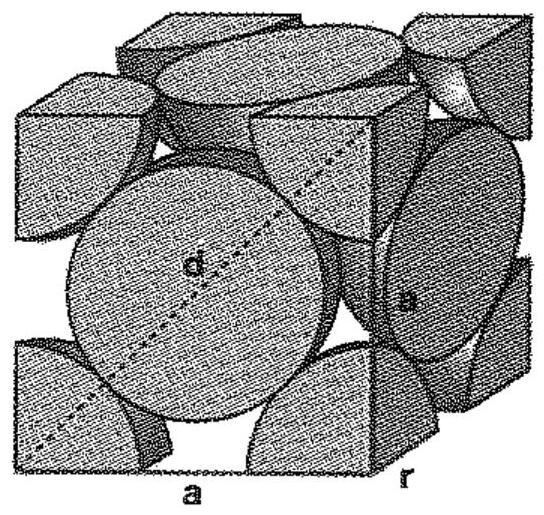
\includegraphics[max width=\textwidth, center]{2025_10_23_74efce88ce3a451fd6b0g-100}\\
d) Các quả cầu Cu chiếm $74 \%$ thể tích trong tinh thể.\\
27.47. Theo QCVN 01-1:2018/BYT, hàm lượng sắt tối đa cho phép trong nước sinh hoạt là $0,30 \mathrm{mg} / \mathrm{L}$.\\
Một mẫu nước có hàm lượng sắt cao gấp 28 lần ngưỡng cho phép, giả thiết sắt trong mẫu nước tồn tại ở dạng $\mathrm{Fe}_{2}\left(\mathrm{SO}_{4}\right)_{3}$ và $\mathrm{FeSO}_{4}$ với tỉ lệ mol tương ứng là $1: 8$. Quá trình tách loại sắt trong $10 \mathrm{~m}^{3}$ mẫu nước trên được thực hiện bằng cách sử dụng m gam vôi tôi (vừa đủ) để tăng pH , sau đó sục không khí:


\begin{equation*}
\mathrm{Fe}_{2}\left(\mathrm{SO}_{4}\right)_{3}+\mathrm{Ca}(\mathrm{OH})_{2} \longrightarrow \mathrm{Fe}(\mathrm{OH})_{3}+\mathrm{CaSO}_{4} \tag{1}
\end{equation*}



\begin{equation*}
\mathrm{FeSO}_{4}+\mathrm{Ca}(\mathrm{OH})_{2}+\mathrm{O}_{2}+\mathrm{H}_{2} \mathrm{O} \longrightarrow \mathrm{Fe}(\mathrm{OH})_{3}+\mathrm{CaSO}_{4} \tag{2}
\end{equation*}


Giả thiết vôi tôi chỉ chứa $\mathrm{Ca}(\mathrm{OH})_{2}$. Giá trị của m là bao nhiêu? (Làm tròn kết quả đến phần nguyên).\\
27.48. Các nghiên cứu được thực hiện với một muối carbonate của kim loại M (hoá trị II) như sau.\\
Nghiên cứu 1: Tiến hành phân tích hàm lượng các nguyên tố, xác định M chiếm $48,28 \%$ khối lượng muối.\\
Nghiên cứu 2: Nung nóng muối carbonate tới phản ứng hoàn toàn trong các khí quyển khác nhau:

\begin{center}
\begin{tabular}{|c|c|c|c|}
\hline
Thinghem & 1 & 2 & 3 \\
\hline
Xhiquyen & $\mathrm{N}_{2}$ & $\mathrm{O}_{2}$ & HCl \\
\hline
\end{tabular}
\end{center}

Phần trăm chênh lệch giữa khối lượng mẫu chất rắn sau khi nung so với muối ban đầu ở thí nghiệm 2 là $\mathrm{a} \%$. Giá trị của a là bao nhiêu? (Làm tròn kết quả đến phần nguyên).\\
27.49. Iron(II) sulfate thường được bảo quản ở dạng muối Mohr màu xanh nhạt có công thức $\mathrm{FeSO}_{4} \cdot\left(\mathrm{NH}_{4}\right)_{2} \mathrm{SO}_{4} \cdot \mathrm{nH}_{2} \mathrm{O}$.\\
Thực hiện các thí nghiệm sau:\\
Thí nghiệm 1: Cân $1,96 \mathrm{~g}$ muối Mohr rồi hoà tan vào nước, sau đó định mức trong bình 50 mL . Chuẩn độ $5,00 \mathrm{~mL}$ dung dịch vừa pha cần dùng $5,00 \mathrm{~mL}$ dung dịch $\mathrm{KMnO}_{4} 0,02 \mathrm{M}$ trong môi trường $\mathrm{H}_{2} \mathrm{SO}_{4}$ loãng. Xác định công thức phân tử muối Mohr.\\
Thí nghiệm 2: Làm lạnh 100 g dung dịch muối Mohr bão hoà ở $30^{\circ} \mathrm{C}$ đến nhiệt độ ổn định ở $0^{\circ} \mathrm{C}$, thu được m gam muối Mohr kết tinh.\\
Cho độ tan của muối Mohr trong nước ở các nhiệt độ như sau:

\begin{center}
\begin{tabular}{|c|c|c|c|c|}
\hline
Nhiet do $(\mathrm{OC})$ & 0 & 10 & 20 & 30 \\
\hline
Dó $\mathrm{tan}(\mathrm{g} / 100 \mathrm{~g}$ nưóc $)$ & 17,2 & 31,0 & 36,4 & 45,0 \\
\hline
\end{tabular}
\end{center}

Giá trị của m là bao nhiêu? (Làm tròn kết quả đến phần mười).

\section*{BÀI 28}
\section*{SO LƯỢC VỀ PHÚC CHẤT}
\section*{NHAN BIET}
28.1. Phối tử trong phức chất $\left[\mathrm{PtCl}_{4}\right]^{2-}$ và $\left[\mathrm{Fe}(\mathrm{CO})_{5}\right]$ lần lượt là\\
A. Cl và C .\\
B. Pt và Fe .\\
C. $\mathrm{Cl}^{-}$và CO .\\
D. Cl và CO .\\
28.2. Số lượng phối tử có trong mỗi phức chất $\left[\mathrm{PtCl}_{4}\right]^{2-},\left[\mathrm{Fe}(\mathrm{CO})_{5}\right]$ lần lượt là\\
A. 4 và 5 .\\
B. 5 và 6 .\\
C. 2 và 5 .\\
D. 1 và 2 .\\
28.3. Nguyên tử trung tâm của phức chất $\left[\mathrm{PtCl}_{4}\right]^{2-}$ và $\left[\mathrm{Fe}(\mathrm{CO})_{5}\right]$ lần lượt là\\
A. $\mathrm{Pt}^{4+}$ và $\mathrm{Fe}^{2+}$.\\
B. $\mathrm{Pt}^{2+}$ và $\mathrm{Fe}^{2+}$.\\
$\mathrm{C} . \mathrm{Cl}$ và CO .\\
D. $\mathrm{Pt}^{2+}$ và Fe .\\
28.4. Điện tích của phức chất $\left[\mathrm{PtCl}_{4}\right]^{2-}$ và $\left[\mathrm{Fe}(\mathrm{CO})_{5}\right]$ lần lượt là\\
A. +2 và +5 .\\
B. +2 và 0 .\\
C. -1 và 0 .\\
D. -2 và 0 .\\
28.5. Công thức tổng quát của phức chất (với nguyên tử trung tâm M và phối tử L ) có dạng tứ diện và bát diện lần lượt là\\
A. $\left[\mathrm{ML}_{2}\right]$ và $\left[\mathrm{ML}_{4}\right]$.\\
B. $\left[\mathrm{ML}_{4}\right]$ và $\left[\mathrm{ML}_{6}\right]$.\\
C. $\left[\mathrm{ML}_{6}\right]$ và $\left[\mathrm{ML}_{2}\right]$.\\
D. $\left[\mathrm{ML}_{6}\right]$ và $\left[\mathrm{ML}_{4}\right]$.\\
28.6. Chọn đáp án đúng nhất về dạng hình học có thể có của phức chất có công thức tổng quát $\left[\mathrm{ML}_{4}\right]$.\\
A. Tứ diện.\\
B. Bát diện.\\
C . Vuông phẳng.\\
D. Tứ diện hoặc vuông phẳng.\\
28.7. Phức chất $\left[\mathrm{Cu}\left(\mathrm{H}_{2} \mathrm{O}\right)_{6}\right]^{2+}$ có dạng hình học là\\
A. vuông phẳng.\\
B. tứ diện.\\
C. bát diện.\\
D. đường thẳng.\\
28.8. Chọn đáp án đúng nhất sau về liên kết trong phức chất $\left[\mathrm{PtCl}_{4}\right]^{2-}$.\\
A. Là liên kết cộng hoá trị được hình thành do sự cho cặp electron chưa liên kết từ phối tử $\mathrm{Cl}^{-}$vào nguyên tử trung tâm $\mathrm{Pt}^{2+}$.\\
B. Là liên kết cộng hoá trị được hình thành do sự cho cặp electron chưa liên kết từ nguyên tử trung tâm $\mathrm{Pt}^{2+}$ vào phối tử $\mathrm{Cl}^{-}$.\\
C. Là liên kết tĩnh điện giữa nguyên tử trung tâm $\mathrm{Pt}^{2+}$ và phối tử $\mathrm{Cl}^{-}$.\\
D. Là liên kết cộng hoá trị được hình thành do sự ghép đôi cặp electron của phối tử $\mathrm{Cl}^{-}$và nguyên tử trung tâm $\mathrm{Pt}^{2+}$.

\section*{THONG HIEU}
28.9. Điện tích của nguyên tử trung tâm trong phức chất $\left[\mathrm{Co}\left(\mathrm{NH}_{3}\right)_{6}\right]^{3+}$ và $\left[\mathrm{FeF}_{6}\right]^{3-}$ lần lượt là\\
A. +3 và +3 .\\
B. +3 và +2 .\\
C. +6 và -6 .\\
D. +3 và -3 .\\
28.10. Dạng hình học có thể có của phức chất $\left[\mathrm{FeF}_{6}\right]^{3-}$ là\\
A. tứ diện.\\
B. bát diện.\\
C. vuông phẳng.\\
D. tứ diện hoặc vuông phẳng.

Hãy chọn đúng hoăc sai cho mỗí ý $\mathrm{a}, \mathrm{b}, \mathrm{c}, \mathrm{d}$ ở các câu $28.11-28.13$.\\
28.11. Xét phức chất $\left[\mathrm{CoCl}_{2}\left(\mathrm{NH}_{3}\right)_{4}\right]^{+}$.\\
a) Nguyên từ trung tâm trong phức chất là $\mathrm{Co}^{2+}$.\\
b) Các phối tử có trong phức chất là $\mathrm{Cl}^{-}, \mathrm{NH}_{3}$.\\
c) Số lượng phối tử trong phức chất là 6 .\\
d) Điện tích của phức chất là +3 .\\
28.12. Xét phức chất $\left[\mathrm{ZnCl}_{4}\right]^{2+}$.\\
a) Số lượng phối tử trong phức chất là 2 .\\
b) Liên kết trong phức chất được hình thành là do phối tử $\mathrm{Cl}^{-}$cho cặp electron chưa liên kết vào nguyên tử trung tâm $\mathrm{Zn}^{2+}$.\\
c) Điện tích của phức chất là +3.\\
d) Phức chất có thể có dạng hình học bát diện.\\
28.13. Xét phức chất $\left[\mathrm{Ni}\left(\mathrm{NH}_{3}\right)_{6}\right]^{2+}$.\\
a) Phức chất có thể có dạng hình học tứ diện hoặc vuông phẳng.\\
b) Liên kết trong phức chất được hình thành là do phối tử $\mathrm{NH}_{3}$ cho cặp electron chưa liên kết vào nguyên tử trung tâm $\mathrm{Ni}^{+}$.\\
c) Nguyên tử trung tâm trong phức chất là $\mathrm{Ni}^{2+}$.\\
d) Điện tích của phức chất là +2 .\\
28.14. Số lượng phối tử trong phức chất $\left[\mathrm{PtCl}_{4}\left(\mathrm{NH}_{3}\right)_{2}\right]^{2-}$ là bao nhiêu?\\
28.15. Hãy cho biết điện tích của phức chất $\left[\mathrm{PtCl}_{4}\left(\mathrm{NH}_{3}\right)_{2}\right]^{2-}$.

\section*{VAN DUNG}
28.16. Phức chất $\left[\mathrm{MA}_{\mathrm{x}} \mathrm{B}_{\mathrm{y}}\right]$ có dạng hình học vuông phẳng. Ở đó M là nguyên tử trung tâm, $x$ và $y$ là số phối tử của $A$ và $B$. Giá trị của $x+y$ là bao nhiêu?\\
28.17. Phức chất $\left[\mathrm{MA}_{\mathrm{X}} \mathrm{B}_{2}\right]$ có dạng hình học tứ diện. Ở đó M là nguyên tử trung tâm, $x$ là số phối tử của $A$. Giá trị của $x$ là bao nhiêu?\\
28.18. Phức chất $\left[\mathrm{MA}_{\mathrm{X}} \mathrm{B}_{2}\right]$ có dạng hình học bát diện. Ở đó M là nguyên tử trung tâm, x là số phối tử của A . Giá trị của x là bao nhiêu?\\
Hãy chọn đúng hoặc sai cho mỗi ý a, b, c, d ở câu sau.\\
28.19. Trong dung dịch $\mathrm{Fe}^{3+}$ tạo phức chất aqua có dạng hình học bát diện.\\
a) Công thức hoá học của phức chất là $\left[\mathrm{Fe}\left(\mathrm{H}_{2} \mathrm{O}\right)_{6}\right]^{2+}$.\\
b) Phức chất có điện tích là +2 .\\
c) Số lượng phối tử trọng phức chất là 6 .\\
d) Liên kết trong phức chất được hình thành là do phối tử $\mathrm{H}_{2} \mathrm{O}$ cho cặp electron chưa liên kết vào nguyên tử trung tâm $\mathrm{Fe}^{3+}$.

\section*{BÀI 29}
\section*{MỘT SỐ TÍNH CHẤT VÀ ÚNG DỤNG CỦA PHỨC CHẤT}
\section*{NHAN BIÉT}
29.1. Phức chất nào sau đây của $\mathrm{Cu}^{2+}$ có màu vàng?\\
A. $\left[\mathrm{Cu}\left(\mathrm{H}_{2} \mathrm{O}\right)_{6}\right]^{2+}$.\\
B. $\left[\mathrm{CuCl}_{4}\right]^{2-}$.\\
C. $\left[\mathrm{Cu}\left(\mathrm{NH}_{3}\right)_{4}\left(\mathrm{H}_{2} \mathrm{O}\right)_{2}\right]$.\\
D. $\left[\mathrm{Cu}(\mathrm{OH})_{2}\left(\mathrm{H}_{2} \mathrm{O}\right)_{4}\right]$.\\
29.2. Hai ống nghiệm (1) và (2) đều chứa phức chất của $\mathrm{Cu}^{2+}$. Ông nghiệm (1) có màu xanh lam, ống nghiệm (2) có màu xanh nhạt. Ống nghiệm (1) và (2) lần lượt chứa phức chất là\\
A. $\left[\mathrm{Cu}\left(\mathrm{H}_{2} \mathrm{O}\right)_{6}\right]^{2+}$ và $\left[\mathrm{Cu}\left(\mathrm{NH}_{3}\right)_{4}\left(\mathrm{H}_{2} \mathrm{O}\right)_{2}\right]$.\\
B. $\left[\mathrm{Cu}\left(\mathrm{H}_{2} \mathrm{O}\right)_{6}\right]^{2+}$ và $\left[\mathrm{CuCl}_{4}\right]^{2}$.\\
C. $\left[\mathrm{CuCl}_{4}\right]^{2-}$ và $\left[\mathrm{Cu}\left(\mathrm{NH}_{3}\right)_{4}\left(\mathrm{H}_{2} \mathrm{O}\right)_{2}\right]$.\\
D. $\left[\mathrm{Cu}\left(\mathrm{NH}_{3}\right)_{4}\left(\mathrm{H}_{2} \mathrm{O}\right)_{2}\right]$ và $\left[\mathrm{Cu}\left(\mathrm{H}_{2} \mathrm{O}\right)_{6}\right]^{2+}$.\\
29.3. Nhỏ vài giọt dung dịch HCl đặc vào dung dịch $\mathrm{CuSO}_{4}$ tạo thành phức chất $\left[\mathrm{CuCl}_{4}\right]^{2-}$. Dấu hiệu nào sau đây chứng tỏ phức chất $\left[\mathrm{CuCl}_{4}\right]^{2-}$ tạo thành?\\
A. Hoà tan kết tủa.\\
B. Đổi màu dung dịch từ màu xanh sang màu vàng.\\
C. Xuất hiện kết tủa.\\
D. Đổi màu dung dịch từ màu xanh lam sang màu vàng.\\
29.4. Cho lượng dư dung dịch $\mathrm{NH}_{3}$ tác dụng với AgCl . Phát biểu nào sau đây đúng?\\
A. Kết tủa trắng tan dần, phức chất $\left[\mathrm{Ag}\left(\mathrm{NH}_{3}\right)_{2}\right]^{+}$không màu được tạo thành.\\
B. Không có hiện tượng gì xảy ra.\\
C. Kết tủa trắng tan dần, phức chất $\left[\mathrm{Ag}\left(\mathrm{NH}_{3}\right)_{2}\right]^{+}$màu xanh được tạo thành.\\
D. Kết tủa trắng tan dần, phức chất $\left[\mathrm{Ag}\left(\mathrm{NH}_{3}\right)_{4}\right]^{+}$không màu được tạo thành.\\
29.5. Nhỏ vài giọt dung dịch NaOH loãng vào dung dịch $\mathrm{CuSO}_{4}$ tạo thành phức chất $\left[\mathrm{Cu}(\mathrm{OH})_{2}\left(\mathrm{H}_{2} \mathrm{O}\right)_{4}\right]$. Dấu hiệu nào sau đây chứng tỏ phức chất [ $\mathrm{Cu}(\mathrm{OH})_{2}\left(\mathrm{H}_{2} \mathrm{O}\right)_{4}$ ] tạo thành?\\
A. Xuất hiện kết tủa màu xanh lam.\\
B. Hoà tan kết tủa.\\
C. Dung dịch chuyển từ màu xanh sang màu vàng.\\
D. Xuất hiện kết tủa màu xanh nhạt.\\
29.6. Phát biểu nào sau đây đúng?\\
A. Phức chất aqua là phức chất chứa phối tử $\mathrm{NH}_{3}$.\\
B. Phức chất của kim loại chuyển tiếp đều tan trong dung dịch.\\
C. Muối $\mathrm{CuSO}_{4}$ khan màu trắng khi tan vào nước tạo thành dung dịch có màu xanh do tạo thành phức chất aqua $\left[\mathrm{Cu}\left(\mathrm{H}_{2} \mathrm{O}\right)_{6}\right]^{2+}$.\\
D. Phức chất của kim loại chuyển tiếp đều có màu.\\
29.7. Phát biểu nào sau đây không đúng?\\
A. Trong dung dịch, các ion kim loại chuyển tiếp đều tạo phức chất aqua.\\
B. Các phối tữ $\mathrm{H}_{2} \mathrm{O}$ trong phức chất aqua không thể bị thế bởi các phối tử khác.\\
C. Phức chất aqua của các ion kim loại chuyển tiếp hầu hết có dạng hình học bát diện.\\
D. Các phối tử trong phức chất có thể bị thay thế một phần hoặc thay thế hết bởi các phối tử khác.\\
29.8. Các phối tử $\mathrm{H}_{2} \mathrm{O}$ trong phức chất $\left[\mathrm{Ni}\left(\mathrm{H}_{2} \mathrm{O}\right)_{6}\right]^{2+}$ có thể bị thế hết bởi sáu phối tử $\mathrm{NH}_{3}$ tạo thành phức chất là\\
A. $\left[\mathrm{Ni}\left(\mathrm{NH}_{3}\right)_{6}\right]^{2+}$.\\
B. $\left[\mathrm{Ni}\left(\mathrm{NH}_{3}\right)_{2}\left(\mathrm{H}_{2} \mathrm{O}\right)_{4}\right]$.\\
C. $\left[\mathrm{Ni}\left(\mathrm{NH}_{3}\right)\left(\mathrm{H}_{2} \mathrm{O}\right)_{5}\right]^{2+}$.\\
D. $\left[\mathrm{Ni}\left(\mathrm{NH}_{3}\right)_{5}\left(\mathrm{H}_{2} \mathrm{O}\right)\right]^{2+}$.\\
29.9. Phối tử $\mathrm{H}_{2} \mathrm{O}$ trong phức chất aqua $\left[\mathrm{Cu}\left(\mathrm{H}_{2} \mathrm{O}\right)_{6}\right]^{2+}$ có thể bị thế bởi 1 phối tử $\mathrm{NH}_{3}$ tạo thành phức chất là\\
A. $\left[\mathrm{Cu}\left(\mathrm{NH}_{3}\right)_{6}\right]^{2+}$.\\
B. $\left[\mathrm{Cu}\left(\mathrm{NH}_{3}\right)_{2}\left(\mathrm{H}_{2} \mathrm{O}\right)_{5}\right]$.\\
C. $\left[\mathrm{Cu}\left(\mathrm{NH}_{3}\right)\left(\mathrm{H}_{2} \mathrm{O}\right)_{5}\right]^{2+}$\\
D. $\left[\mathrm{Cu}\left(\mathrm{NH}_{3}\right)\left(\mathrm{H}_{2} \mathrm{O}\right)_{5}\right]^{+}$\\
29.10. Phát biểu nào sau đây đúng?\\
A. Các phối tử trong phức chất chỉ có thể bị thế một phần bởi các phối tử khác.\\
B. Các phối tử trong phức chất chỉ có thể bị thế tất cả bởi các phối tử khác.\\
C. Tất cả các phức chất aqua đều kém tan trong nước.\\
D. Phức chất được dùng làm thuốc chữa bệnh ung thư với tên gọi thương phẩm là cisplatin có công thức hoá học là $\left[\mathrm{PtCl}_{2}\left(\mathrm{NH}_{3}\right)_{2}\right]$.

\section*{THONG MIEU}
29.11. Phức chất $\left[\mathrm{Cu}\left(\mathrm{H}_{2} \mathrm{O}\right)_{6}\right]^{2+}$ có màu xanh; phức chất $\left[\mathrm{Cu}\left(\mathrm{NH}_{3}\right)_{4}\left(\mathrm{H}_{2} \mathrm{O}\right)_{2}\right]$ có màu xanh lam và phức chất $\left[\mathrm{CuCl}_{4}\right]^{2-}$ có màu vàng. Màu sắc của ba phức chất khác nhau là do chúng khác nhau về\\
A. nguyên tử trung tâm.\\
B. phối tử.\\
C. cả nguyên tử trung tâm và phối tử.\\
D. số lượng phối tử.\\
29.12. Trong phức chất $\left[\mathrm{Co}\left(\mathrm{H}_{2} \mathrm{O}\right)_{6}\right]^{2+}, 2$ phối tử $\mathrm{H}_{2} \mathrm{O}$ có thể bị thế bởi 2 phối tử $\mathrm{OH}^{-}$. Phát biểu nào sau đây không đúng?\\
A. Phức chất tạo thành có 4 phối tử nước và 2 phối tữ $\mathrm{OH}^{-}$.\\
B. Phức chất tạo thành có điện tích +2 .\\
C. Phức chất tạo thành có nguyên tử trung tâm là $\mathrm{Co}^{2+}$.\\
D. Phức chất tạo thành là $\left[\mathrm{Co}(\mathrm{OH})_{2}\left(\mathrm{H}_{2} \mathrm{O}\right)_{4}\right]$.

Hãy chọn đúng hoặc sai cho mỗi ý à b, c, d ở các câu 29.13-29.19.\\
29.13. Phức chất $\left[\mathrm{Cu}\left(\mathrm{H}_{2} \mathrm{O}\right)_{6}\right]^{2+},\left[\mathrm{Cu}\left(\mathrm{NH}_{3}\right)_{4}\left(\mathrm{H}_{2} \mathrm{O}\right)_{2}\right]$ và $\left[\mathrm{Co}\left(\mathrm{H}_{2} \mathrm{O}\right)_{6}\right]^{2+}$ có màu xanh, xanh lam và hồng đỏ.\\
a) Các phức chất có cùng nguyên tử trung tâm có màu sắc giống nhau.\\
b) Các phức chất có cùng phối tử có màu sắc giống nhau.\\
c) Màu sắc của phức chất không phụ thuộc vào bản chất của nguyên tử trung tâm và phối tử.\\
d) Màu sắc của phức chất phụ thuộc vào bản chất của nguyên tử trung tâm và phối tử.\\
29.14. Thực hiện thí nghiệm cho dung dịch $\mathrm{NH}_{3}$ vào ống nghiệm đựng bột $\mathrm{Ni}(\mathrm{OH})_{2}$ màu xanh lá cây đến dư, thu được phức chất bát diện chỉ chứa phối tử $\mathrm{NH}_{3}$ có màu xanh dương.\\
a) Phức chất $\left[\mathrm{Ni}\left(\mathrm{NH}_{3}\right)_{6}\right]^{2+}$ được tạo thành.\\
b) Dấu hiệu nhận biết phức chất tạo thành là kết tủa màu xanh lá cây bị tan ra.\\
c) Phức chất thu được chứa bốn phối tử $\mathrm{NH}_{3}$.\\
d) Phức chất thu được có nguyên tử trung tâm là $\mathrm{Ni}^{2+}$.\\
29.15. Cho $\mathrm{CuSO}_{4}$ khan không màu vào nước được dung dịch phức chất A màu xanh. Nhỏ từ từ dung dịch $\mathrm{NH}_{3}$ đặc vào dung dịch A , lúc đầu thấy xuất hiện kết tủa phức chất B màu xanh nhạt, sau đó kết tủa tan dần tạo thành dung dịch phức chất C màu xanh lam.\\
a) Phức chất A là $\left[\mathrm{Cu}\left(\mathrm{H}_{2} \mathrm{O}\right)_{6}\right]^{2+}$.\\
b) Phức chất B là $\left[\mathrm{Cu}\left(\mathrm{NH}_{3}\right)_{4}\left(\mathrm{H}_{2} \mathrm{O}\right)_{2}\right]^{2+}$.\\
c) Phức chất C là $\left[\mathrm{Cu}(\mathrm{OH})_{2}\left(\mathrm{H}_{2} \mathrm{O}\right)_{4}\right]$.\\
d) Dấu hiệu nhận biết sự tạo thành phức chất C là: hoà tan kết tủa và đổi màu dung dịch.\\
29.16. Thực hiện hai thí nghiệm liên tiếp: (1) nhỏ từ từ dung dịch NaCl vào ống nghiệm đựng dung dịch $\mathrm{AgNO}_{3}$; (2) sau đó nhỏ thêm dung dịch $\mathrm{NH}_{3}$ đến dư vào ống nghiệm.\\
a) Phức chất AgCl kết tủa trắng được tạo thành ở thí nghiệm (1).\\
b) Phức chất $\left[\mathrm{Ag}\left(\mathrm{NH}_{3}\right)_{2}\right]^{+}$không màu được tạo thành ở thí nghiệm (2).\\
c) Dấu hiệu nhận biết phức chất $\left[\mathrm{Ag}\left(\mathrm{NH}_{3}\right)_{2}\right]^{+}$tạo thành là kết tủa tan.\\
d) Phức chất được tạo thành ở thí nghiệm (2) chứa bốn phối tử $\mathrm{NH}_{3}$.\\
29.17. Có 4 lọ hoá chất mất nhãn, mỗi lọ đựng dung dịch của một trong các phức chất sau: $\left[\mathrm{Ag}\left(\mathrm{NH}_{3}\right)_{2}\right]^{+},\left[\mathrm{CuCl}_{4}\right]^{2-},\left[\mathrm{Fe}\left(\mathrm{H}_{2} \mathrm{O}\right)_{6}\right]^{2+},\left[\mathrm{Cu}\left(\mathrm{NH}_{3}\right)_{4}\left(\mathrm{H}_{2} \mathrm{O}\right)_{2}\right]^{2+}$.\\
a) Lọ không có màu đựng phức chất $\left[\mathrm{Ag}\left(\mathrm{NH}_{3}\right)_{2}\right]^{+}$.\\
b) Lọ có màu da cam đựng phức chất $\left[\mathrm{Fe}\left(\mathrm{H}_{2} \mathrm{O}\right)_{6}\right]^{2+}$.\\
c) Lọ có màu xanh lam đựng phức chất $\left[\mathrm{Cu}\left(\mathrm{NH}_{3}\right)_{4}\left(\mathrm{H}_{2} \mathrm{O}\right)_{2}\right]^{2+}$.\\
d) Lọ có màu xanh nhạt đựng phức chất $\left[\mathrm{CuCl}_{4}\right]^{2-}$.\\
29.18. Xét phản úng sau: $\left[\mathrm{Cu}\left(\mathrm{H}_{2} \mathrm{O}\right)_{6}\right]^{2+}+\mathrm{NH}_{3} \longrightarrow\left[\mathrm{Cu}\left(\mathrm{NH}_{3}\right)\left(\mathrm{H}_{2} \mathrm{O}\right)_{5}\right]^{2+}$\\
a) Phản ứng thuộc loại phản ứng oxi hoá - khử.\\
b) 1 phối tử nước trong phức chất $\left[\mathrm{Cu}\left(\mathrm{H}_{2} \mathrm{O}\right)_{6}\right]^{2+}$ đã bị thế bởi 1 phối tử $\mathrm{NH}_{3}$.\\
c) Dấu hiệu của phức chất $\left[\mathrm{Cu}\left(\mathrm{NH}_{3}\right)\left(\mathrm{H}_{2} \mathrm{O}\right)_{5}\right]^{2+}$ tạo thành là tạo thành kết tủa.\\
d) Phức chất tạo thành có tổng 6 phối tử.\\
29.19. Trong dung dịch, ion $\mathrm{Fe}^{3+}$ tồn tại dưới dạng phức chất aqua có sáu phối tử nước.\\
a) Phức chất aqua có công thức hoá học là $\left[\mathrm{Fe}\left(\mathrm{H}_{2} \mathrm{O}\right)_{6}\right]^{3+}$.\\
b) Phức chất aqua có dạng hình học vuông phẳng.\\
c) 6 phối tử nước đã cho cặp electron chưa liên kết vào ion $\mathrm{Fe}^{3+}$.\\
d) Nguyên tử trung tâm trong phức chất aqua là $\mathrm{Fe}^{2+}$.\\
29.20. Phức chất $\left[\mathrm{Pt}\left(\mathrm{NH}_{3}\right)_{4}\right]^{2+}$ có thể bị thế bởi 1 phối tử $\mathrm{Cl}^{-}$. Phức chất tạo thành có điện tích là bao nhiêu?

\section*{VAN DUNG}
Hãy chọn đúng hoăc sai cho mỗi ý a, b, c, d ỏ các câu 29.21-29.23.\\
29.21. Phức chất có vai trò quan trọng làm xúc tác trong tổng hợp hữu cơ. Minh chứng cho vai trò to lớn đó là giải Nobel được trao cho ba nhà khoa học R. F. Heck, E. Negishi và A. Suzuki năm 2010 về phản ứng ghép mạch $\mathrm{C}=\mathrm{C}$ sử dụng xúc tác là phức chất $\left[\mathrm{Pd}\left(\mathrm{P}\left(\mathrm{C}_{6} \mathrm{H}_{5}\right)_{3}\right)_{4}\right]$, còn được gọi là Tetrakis.\\
a) Phức chất Tetrakis có 4 phối tử triphenylphosphine $\left(\mathrm{P}\left(\mathrm{C}_{6} \mathrm{H}_{5}\right)_{3}\right)$.\\
b) Phức chất Tetrakis có dạng hình học bát diện.\\
c) Trong phức chất Tetrakis, nguyên tử trung tâm Pd đã nhận 4 cặp electron của các phối tử.\\
d) Nguyên tử trung tâm trong phức chất Tetrakis là $\mathrm{Pd}^{2+}$.\\
29.22. Nhỏ muối thiocyanate ( $\mathrm{SCN}^{-}$) vào dung dịch muối $\mathrm{Fe}^{3+}$ loãng, dung dịch từ màu vàng nhạt chuyển sang màu đỏ máu là do 1 phối tử nước trong phức chất aqua có dạng hình học bát diện của $\mathrm{Fe}^{3+}$ bị thay thế bởi 1 phối tử $\mathrm{SCN}^{-}$.\\
a) Phức chất aqua có công thức hoá học là $\left[\mathrm{Fe}\left(\mathrm{H}_{2} \mathrm{O}\right)_{6}\right]^{3+}$.\\
b) Phức chất có màu đỏ máu là phức chất của $\mathrm{Fe}^{3+}$ có chứa 1 phối tử $\mathrm{SCN}^{-}$và 6 phối tử nước.\\
c) Phức chất màu đỏ máu có công thức hoá học là $\left[\mathrm{Fe}\left(\mathrm{H}_{2} \mathrm{O}\right)_{5}(\mathrm{SCN})\right]^{2+}$.\\
d) Phức chất màu đỏ máu có điện tích +3 .\\
29.23. Cho các hoá chất sau: HCl đặc; $\mathrm{NH}_{3} 10 \% ; \mathrm{CuSO}_{4}$ khan; nước.\\
a) Có thể điều chế được phức chất $\left[\mathrm{Cu}\left(\mathrm{H}_{2} \mathrm{O}\right)_{6}\right]^{2+}$ bằng cách hoà tan $\mathrm{CuSO}_{4}$ khan vào nước.\\
b) Hoà tan $\mathrm{CuSO}_{4}$ khan trong nước, dung dịch thu được cho tác dụng với HCl đặc thu được phức chất $\left[\mathrm{CuCl}_{4}\right]^{2-}$ có dạng hình học bát diện.\\
c) Không thể điều chế được phức chất $\left[\mathrm{Cu}(\mathrm{OH})_{2}\left(\mathrm{H}_{2} \mathrm{O}\right)_{4}\right]$.\\
d) Hoà $\mathrm{CuSO}_{4}$ khan trong nước, dung dịch thu được cho tác dụng với dung dịch $\mathrm{NH}_{3} 10 \%$, thu được phức chất $\left[\mathrm{Cu}\left(\mathrm{NH}_{3}\right)_{4}\left(\mathrm{H}_{2} \mathrm{O}\right)_{2}\right]$ có dạng hình học bát diện.\\
29.24. Cisplatin là thế hệ đầu tiên trong số ba phức chất của $\mathrm{Pt}^{2+}$ được sử dụng trong điều trị ung thư. Nó được biết đến với vai trò to lớn trong điều trị ung thư buồng trứng, tinh hoàn, bàng quang, đầu, cổ,... Nhờ có cisplatin hơn $90 \%$ bệnh nhân ung thư tinh hoàn đã được cứu sống. Cisplatin có thể được điều chế theo sơ đồ sau:\\
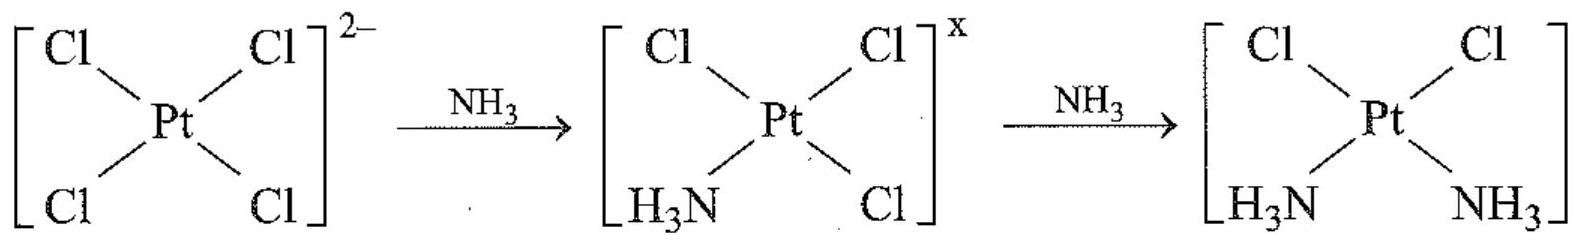
\includegraphics[max width=\textwidth, center]{2025_10_23_74efce88ce3a451fd6b0g-109}

Giá trị của x là bao nhiêu?

\section*{BÀI 30}
\section*{ÔN TẬP CHƯƠNG VIII}
\section*{NHAN BIET}
30.1. Cấu hình electron của $\mathrm{Cu}^{2+}$ là\\
A. $[\mathrm{Ar}] 3 \mathrm{~d}^{9} 4 \mathrm{~s}^{2}$.\\
B. $[\mathrm{Ar}] 3 \mathrm{~d}^{10} 4 \mathrm{~s}^{1}$.\\
C. $[\mathrm{Ar}] 3 \mathrm{~d}^{8} 4 \mathrm{~s}^{1}$.\\
D. $[\mathrm{Ar}] 3 \mathrm{~d}^{9}$.\\
30.2. Phát biểu nào sau đây không đúng?\\
A. Các nguyên tố kim loại chuyển tiếp dãy thứ nhất thuộc khối d.\\
B. Zn là nguyên tử kim loại chuyển tiếp dãy thứ nhất duy nhất có phân lớp 3 d đã điền đầy electron.\\
C. Nguyên tử của các kim loại chuyển tiếp dãy thứ nhất đều có lớp vỏ bên trong của khí hiếm Ar.\\
D. Kim loại chuyển tiếp dãy thứ nhất thường tạo thành các hợp chất với nhiều số oxi hoá khác nhau.\\
30.3. Số lượng phối đử có trong phức chất $\left[\mathrm{PtCl}_{4}\left(\mathrm{NH}_{3}\right)_{2}\right]$ là\\
A. 6 .\\
B. 2 .\\
C. 4 .\\
D. 7 .\\
30.4. Xét phức chất $\left[\mathrm{PtCl}_{2}\left(\mathrm{NH}_{3}\right)_{4}\right]^{2+}$ và $\left[\mathrm{FeF}_{6}\right]^{3-}$.

Phát biểu nào sau đây đúng?\\
A. Số lượng phối tử có trong mỗi phức chất lần lượt là 4 và 6 .\\
B. Điện tích của mỗi phức chất lần lượt là +4 và +3 .\\
C. Nguyên tử trung tâm trong mỗi phức chất là $\mathrm{Pt}^{4+}$ và $\mathrm{Fe}^{3+}$.\\
D. Cả 2 phức chất đều ít tan trong nước.

\section*{THONG HICU}
30.5. Phát biểu nào sau đây không đúng?\\
A. Tất cả các nguyên tố thuộc nhóm B đều là nguyên tố chuyển tiếp dãy thứ nhất.\\
B. Các nguyên tố chuyển tiếp dãy thứ nhất thường có nhiệt độ nóng chảy cao hơn các kim loại nhóm IA và IIA.\\
C. Số oxi hoá của nguyên tử nguyên tố chromium trong hợp chất $\mathrm{K}_{2} \mathrm{CrO}_{4}$ và $\mathrm{K}_{2} \mathrm{Cr}_{2} \mathrm{O}_{7}$ bằng nhau.\\
D. Trạng thái oxi hoá thường gặp của Mn là $+2,+4,+7$.\\
30.6. Phức chất của $\mathrm{Cr}(0)$ có dạng hình học bát diện chỉ chứa phối tử CO có công thức hoá học là\\
A. $\left[\mathrm{Cr}(\mathrm{CO})_{4}\right]$.\\
B. $\left[\mathrm{Cr}(\mathrm{CO})_{6}\right]$.\\
C. $\left[\mathrm{Cr}(\mathrm{CO})_{4}\right]^{2+}$.\\
D. $\left[\mathrm{Cr}(\mathrm{CO})_{6}\right]^{2+}$.

\section*{Hãy chọn đúng hoạc sai cho mỗi ý a, b, c, d ở các câu 30.7-30.8.}
30.7. Thí nghiệm xác định nồng độ muối $\mathrm{Fe}^{2+}$ bằng phương pháp chuẩn độ với dung dịch thuốc tím $\left(\mathrm{KMnO}_{4}\right)$ xảy ra theo phương trình hoá học sau:\\
$10 \mathrm{FeSO}_{4}+2 \mathrm{KMnO}_{4}+8 \mathrm{H}_{2} \mathrm{SO}_{4} \longrightarrow 5 \mathrm{Fe}_{2}\left(\mathrm{SO}_{4}\right)_{3}+\mathrm{K}_{2} \mathrm{SO}_{4}+2 \mathrm{MnSO}_{4}+8 \mathrm{H}_{2} \mathrm{O}$\\
a) Dung dịch thuốc tím được cho vào bình tam giác khi chuẩn độ.\\
b) Dung dịch muối $\mathrm{Fe}^{2+}$ được cho vào burette khi chuẩn độ.\\
c) Phản ứng xảy ra là phản ứng oxi hoá - khử.\\
d) Khi kết thúc chuẩn độ, dung dịch trong bình tam giác có màu hồng tồn tại bền trong khoảng 20 giây là của lượng rất nhỏ $\mathrm{KMnO}_{4}$ dư.\\
30.8. Phức chất có nguyên tử trung tâm $\mathrm{Co}^{2+}$, chứa 4 phối tử $\mathrm{Cl}^{-}$và 2 phối tử $\mathrm{NH}_{3}$.\\
a) Công thức hoá học của phức chất là $\left[\mathrm{CoCl}_{4}\left(\mathrm{NH}_{3}\right)_{2}\right]^{2-}$.\\
b) Phức chất có dạng hình học bát diện.\\
c) Phức chất có điện tích là +2.\\
d) Nguyên tữ trung tâm $\mathrm{Co}^{2+}$ nhận 6 cặp electron chưa liên kết từ các phối tử.

\section*{VAN DUNG}
Hãy chọn đúng hoăc sai cho mỗi ý $a, b, c, d$ ở câu sau.\\
30.9. Kim loại chuyển tiếp dãy thứ nhất có nhiều ứng dụng trong cuộc sống và sản xuất như: V được dùng để chế tạo thiết bị làm việc ở nhiệt độ cao; Cr được dùng để chế tạo mũi khoan; Ti được dùng để chế tạo vật liệu hàng không; Cu được dùng để chế tạo dây dẫn điện;...\\
a) V là kim loại có nhiệt độ nóng chảy cao.\\
b) Cr là kim loại cứng nhất trong tất cả các kim loại.\\
c) Ti là kim loại nặng.\\
d) Cu là kim loại dẫn điện tốt nhất trong tất cả các kim loại.\\
30.10. Phức chất $\left.\left[\mathrm{Co}\left(\mathrm{NH}_{3}\right) \mathrm{Cl}_{\mathrm{x}}\right)\right]^{\mathrm{y}-}$ có dạng hình học bát diện, nguyên tử trung tâm là $\mathrm{Co}^{3+}$. Tổng giá trị của x và y là bao nhiêu?\\
30.11. Cho dung dịch $\mathrm{NH}_{3}$ đặc vào dung dịch phức chất $\left[\mathrm{PtCl}_{4}\right]^{2-}$ thu được phức chất có điện tích +1 là do một số phối tử $\mathrm{Cl}^{-}$trong phức $\left[\mathrm{PtCl}_{4}\right]^{2-}$ bị thay thế bởi phối tử $\mathrm{NH}_{3}$. Số lượng phối tử $\mathrm{Cl}^{-}$đã bị thay thế là bao nhiêu?


\end{document}